\documentclass[]{article}

\newcommand{\abbrlabel}[1]{\makebox[3cm][l]{\textbf{#1}\ }} %\dotfill
\newenvironment{abbreviations}{\begin{list}{}{\renewcommand{\makelabel}{\abbrlabel}}}{\end{list}}

\usepackage{graphicx}
\usepackage{mathtools}
\usepackage{url}
\usepackage{subcaption}
\usepackage{cleveref}
\usepackage{appendix}
\usepackage{enumitem}% http://ctan.org/pkg/enumitem

\usepackage{pdfpages}
\usepackage{glossaries}


\usepackage{fancyhdr}

%opening
%\title{\textbf{Master's Thesis} \\ Correct Projection Mapping on - and Interaction Techniques with - %Cloth-based Deformable Surfaces}

%\author{Dan-Adrian Avram}
%\author{\textbf{Academic Supervisors:} Kasper Hornbaek and Esben Pedersen}
\pagestyle{fancy}
%\renewcommand{\sectionmark}[1]{\leftmark{#1}}
\fancyhf{}
%\fancyhead[R]{MyName} % predefined ()
%\fancyhead[R]{\rightmark} % 1. sectionname
%\fancyhead[L]{\leftmark} % 1. sectionname

%\fancypagestyle{plain}{%
%  \fancyhf{}%
%  \renewcommand{\headrulewidth}{0pt}%
%}
% Now set the headers
%\fancyhead[LE,RO]{\footnotesize\rightmark}
%\fancyhead[LO,RE]{\footnotesize \leftmark}
\fancyhead[LE,RO]{\footnotesize \ifthenelse{\isodd{\value{page}}}{\rightmark}{\leftmark}}
\fancyfoot[C]{\thepage}
%{\ifthenelse{\isodd{\value{page}}}{\leftmark}{\rightmark}

\begin{document}
\setcounter{tocdepth}{5}
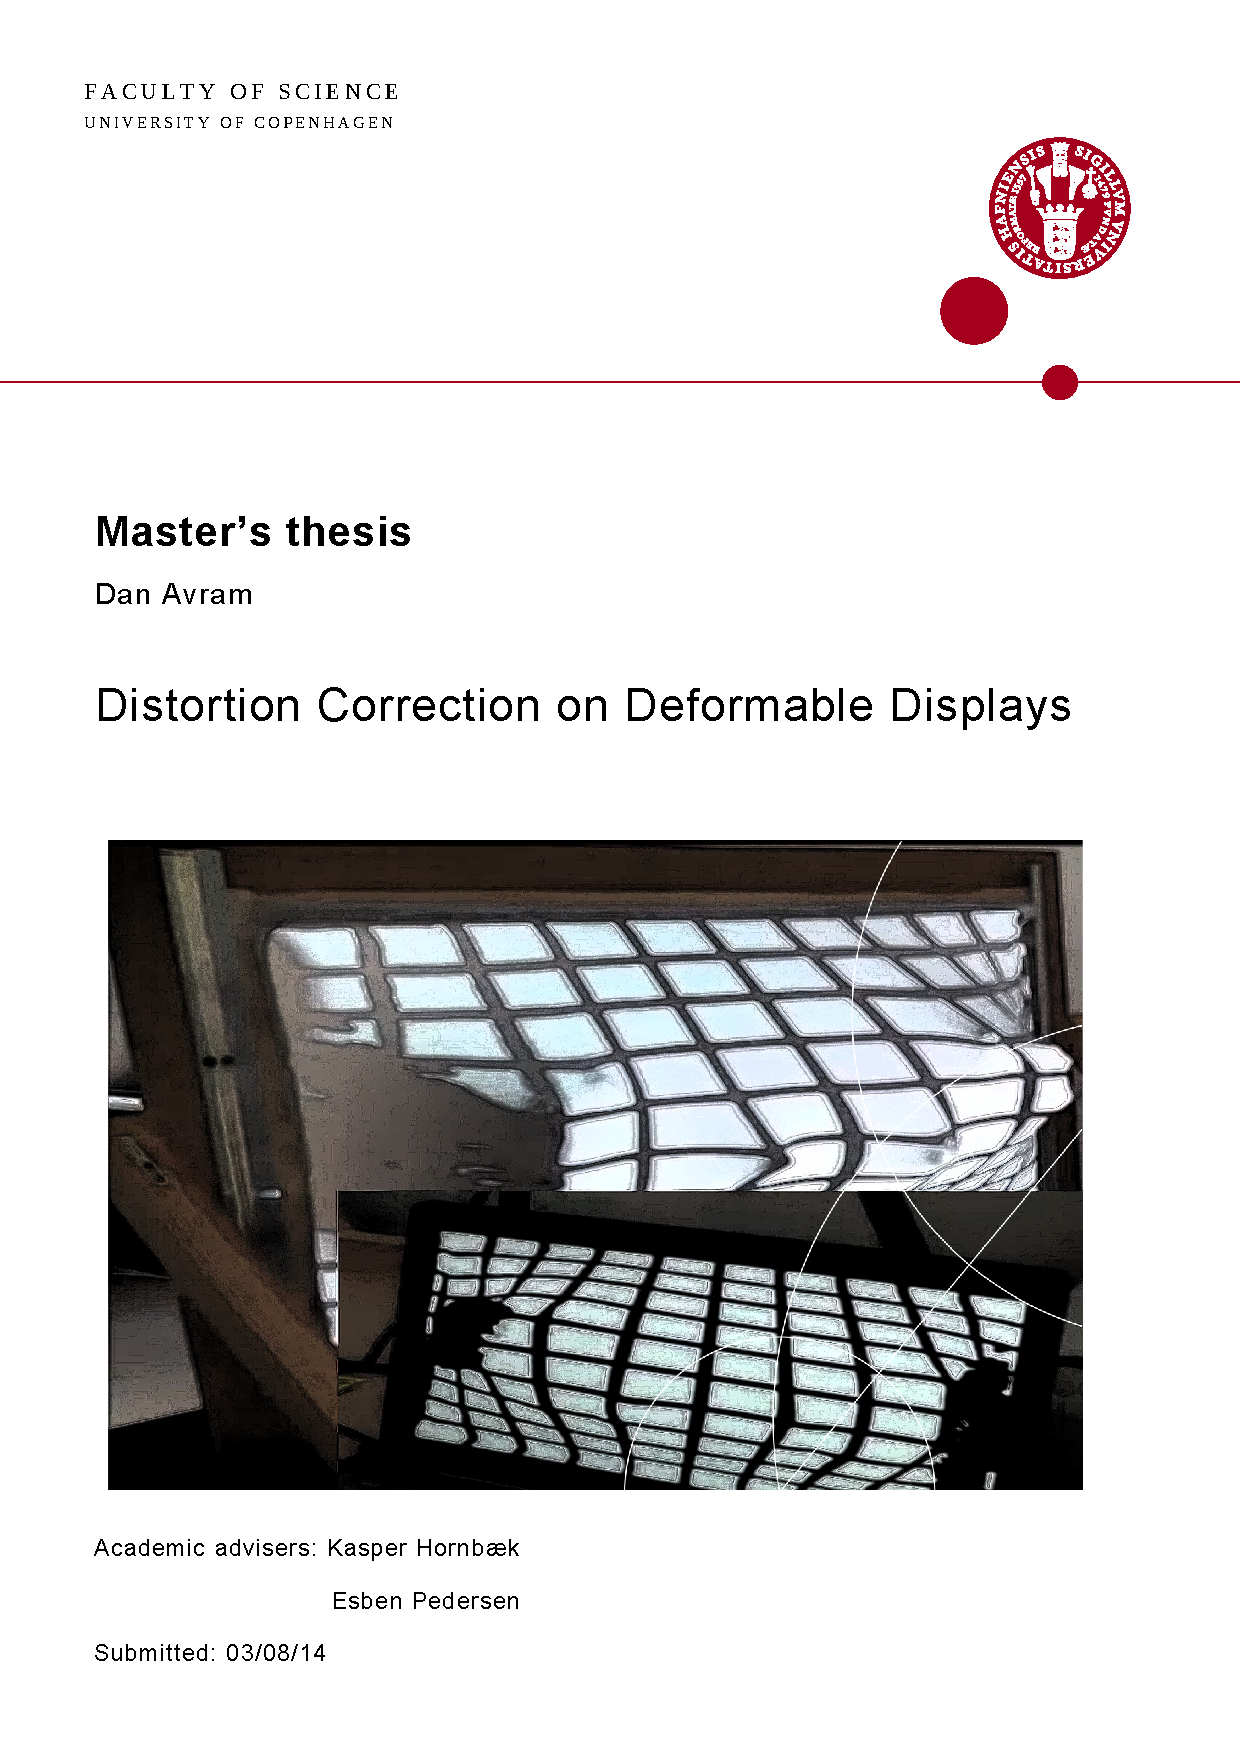
\includepdf[pages={-}]{documents/MScFrontPage.pdf}

%\maketitle
\thispagestyle{empty}
\newpage
\thispagestyle{empty}
\begin{abstract}

In recent years, natural user interfaces have become more and more common. These interfaces are very easy to learn by new users, since they rely on gestures or actions which are already known, unlike physical input devices which have a learning curve. In addition, these artificial input methods also affect the users' experience, since there is an additional layer of abstraction between them and the application. One of the recent important developments, is the growing research around deformable displays. These displays allow the users to interact with an application as they would do in the real world, by directly manipulating the virtual world with their hands. These types of interfaces build upon the touch paradigm, adding an additional layer of flexibility, allowing gestures to be performed in a 3D space. Unlike mid-air methods, these deformable displays also provide haptic feedback while interacting, which can be useful for certain applications.  

One of the main problems with deformable displays is that the image contents become distorted when deforming the surface - the image will follow the shape of the display. For many applications this is not desired: for example, if we want to move an object by pushing and dragging it around, the image should appear as on a flat screen - otherwise the object will also move around and become skewed, due to the deformation induced by the display's shape.

While research has been  done in this area, to my knowledge, the problem is still not completely solved. Although the issue was addressed, for example, in \textit{The Deformable Workspace}, they rely on a custom, dedicated hardware image processor. Further, they only compare some compensated images and videos with normal ones, but they have not done a study to determine how users perceive the compensation. In this project, the aim was to build a distortion correction prototype using off the shelf components. Moreover, an empirical study has been done to determine if participants thought that the compensation is working and if they prefer it over a regular method of displaying the image.

%Unfortunately, the system has a number of limitations. The main issue is that it has not been calibrated, but manually aligned, which means that the compensation is %offset due to misalignments of the physical setup. Several projector-camera calibration techniques were tried, but a workable solution was not employed in the %alloted time. Moreover, even though two methods of noise reduction were applied(spatial and temporal averaging), dynamic artifacts were still present in the final %image, albeit less pronounced. Finally, another issue is that there is some observable latency from the time of interaction, until the image compensates. Although %the image has been updated at around 30 frames per second(\textbf{fps}) with the noise reduction techniques applied, and around 60 fps without.

%These issues all constitute candidates for future work. Finally, the compensation only works well from one viewpoint. In order to fix this issue, the user must be %tracked and the image has to be rotated depending on the viewpoint.

Although the prototype has some limitations, the experiment results indicate both that the compensation is working(to some extent) and that the compensated method was almost universally preferred. For this setup, the results convey that the compensation worked best in the center of the image, because other distortions were introduced on the sides, due to a compensation offset. This issue can be fixed by calibrating the system.

\end{abstract}

\newpage

\renewcommand{\thepage}{\roman{page}}% Roman numerals for page counter
\setcounter{page}{1}
\thispagestyle{empty}
\section*{Glossary}\mbox{}\\

\begin{abbreviations}
\item[CPU] Central Processing Unit
\item[DMA] Direct Memory Access
\item[DOF] Degrees of Freedom
\item[FOV] Field of View
\item[fps] Frames Per Second
\item[GPU] Graphics Processing Unit 
\item[MVP] Model View Projection matrix
\item[NURBS] Non-Uniform Rational B-Spline
\item[QUIS] Questionnaire For User Interaction Satisfaction
\item[PTM] Projective Texture Mapping
\item[SDK] Software Development Kit
\item[TOF] Time of Flight 
\item[VAO] Vertex Array Object 
\item[VBO] Vertex Buffer Object 
\end{abbreviations}
\newpage
\tableofcontents

\newpage
\listoffigures
\newpage
\listoftables 



\newpage
\thispagestyle{empty}
\renewcommand{\thepage}{\arabic{page}}% Arabic numerals for page counter
\setcounter{page}{1}
\section*{Preface}
%\begin{center}
%{\LARGE \textbf{Preface}}\\
%\end{center}
%\bigskip
%\bigskip
This report is the written result of my Master's thesis project at the Department of Computer Science at the University of Copenhagen. 

I would like to thank my academic advisor, Kasper Hornb\ae k as well as my co-advisor, Esben Pedersen, for guidance and feedback throughout the entire project. In addition, I would also like to thank Kenny Erleben for help on computer graphics issues.

Special thanks go to all who participated in the pilot and actual studies as well as to several members of the Human-Centered Computing group, who provided valuable feedback. Finally, I would like to thank my family and friends for their continued support.

\newpage
\section{Introduction}

Deformable displays allow new methods of interaction with virtual scenes, which simply are not possible on flat displays. These interactions are more immersive and feel more natural to the user as they touch, push, pull or pinch the deformable surface. The interaction with the scene can now be done in a 3D space, similarly to how we interact with objects on a daily basis, while also providing a degree of haptic feedback.

Originally, the thesis was split into two parts. The first part of the master thesis project was to deal with the development of a deformable display prototype on which undistorted visuals can be projected, while for the second part there were several alternatives, including investigating gesture interactions and/or affordances in the context of deformable displays. However, the distortion correction issue was more complex than originally thought and it now represents the full focus of the thesis. In addition, the thesis also aimed to gain some insights on how users perceive the distortion correction and whether they would prefer it over the normal image, with distortions that follow the shape of the display.

\subsection{Problem Description}

The distortion of visuals due to irregularities in the surface of an arbitrary-shaped object (the display surface) is the main problem that must be solved. This distortion arises from the user's interaction with the display and represents one of the main challenges when working with deformable surfaces. The image must be changed(the pixels must be shifted) so that the contents still appear as on a flat surface, even when the surface becomes an arbitrary 2.5D object.

If, for example, we are sculpting into or pulling out of a piece of cloth on which visuals are projected, some degree of distortion will appear on the final image. 
The image should be undistorted in the sense that, the visuals would still look like on a fixed display (rather than being deformed with the display), after the previously mentioned pull or pinch gesture is performed. The solution involves tracking of the cloth material and the modeling of a 3D representation of the material that is deformed based on depth sensor data.

In order to solve the problem we need to first setup a scenario where one can test how images are deformed when interacting with deformable displays. In order to do this we need: a surface that can be deformed by a user(e.g.: a cloth material) which serves as our display, a projector that is used to display contents to the end user and a depth camera that is used to track the display and surface and detect changes.

\subsection{Overview}

The report is structured into the following chapters:

\begin{itemize}
\item \textbf{Chapter 2:} Presents related works, mainly in connection with distortion tracking, correction and projection.
\item \textbf{Chapter 3:} The main system components, how they are interconnected and the main theoretical considerations for each part of the system is explained here. Further, alternatives(possible improvements or failed attempts) to employed methods are also discussed in this chapter. There are several reconstruction techniques discussed, but the one that was finally implemented is explained in section \ref{sec:TriangleStripTriangulation}. Further more, several method for calibrating a projector-camera system are also described here. 
\item \textbf{Chapter 4:} In this chapter, the implementation of different parts of the system is discussed. Explanations, main code examples and tests, for the different components of the system are presented here.
\item \textbf{Chapter 5:} The design of the user study is presented here: participants, input, tasks etc.
\item \textbf{Chapter 6:} In this section results are analyzed, both from the empirical study and by directly comparing the visual results of the compensated and uncompensated methods.
\item \textbf{Chapter 7:} Discussion, limitations and possible improvements are mainly described here.
\item \textbf{Chapter 8:} The conclusions to this thesis are presented in this final chapter.
\end{itemize}

Moreover, a video that demonstrates the compensation for all scenarios used in the empirical study, as well as other important aspects of the system is available on the included DVD or on-line(see appendix \ref{appendix:A}). In addition,the full source code is also available. These resources have also been made available online. Finally, the user study documents and thesis resources can be found in the appendices.

\subsection{Hardware Setup}

The deformable display prototype(see figure \ref{fig:hardware_setup}) consists of the following components:
\begin{itemize}
\item Deformable Cloth Display (see Figure \ref{fig:BackViewDeformableDisplay}) + Frame
\begin{figure}[hbtp]
    \centering
    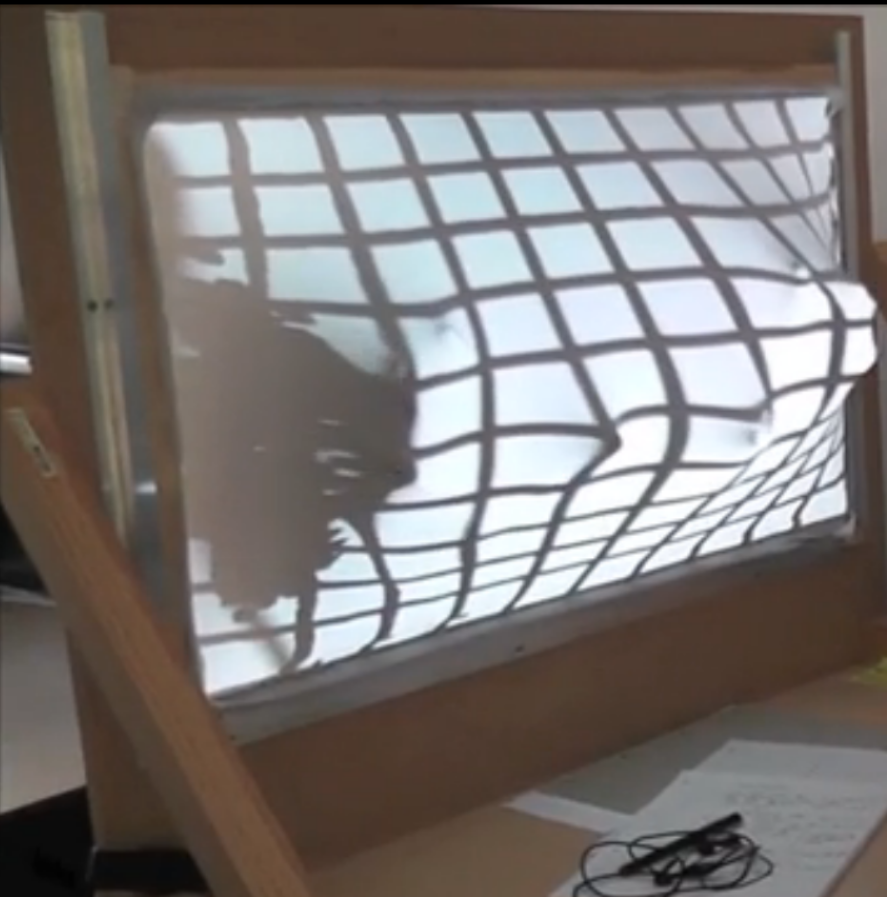
\includegraphics[width=0.6\textwidth]{figures/DisplayBackView.png}
    \caption{Back View of the Deformable Display}
    \label{fig:BackViewDeformableDisplay}
\end{figure}
\item Projector that is used to display the visuals onto the cloth surface\\

A standard projector was used, namely the \textbf{EPSON EWP-TW680}. Through an HDMI signal, it supports up to full-HD resolution, 1920x1080. This corresponds to the screen resolution of the laptop used for development.
\item Depth camera(see Figure \ref{fig:CreativeSenz3D}) that is used to retrieve the cloth display’s depth information\\

\begin{figure}[hbtp]
    \centering
    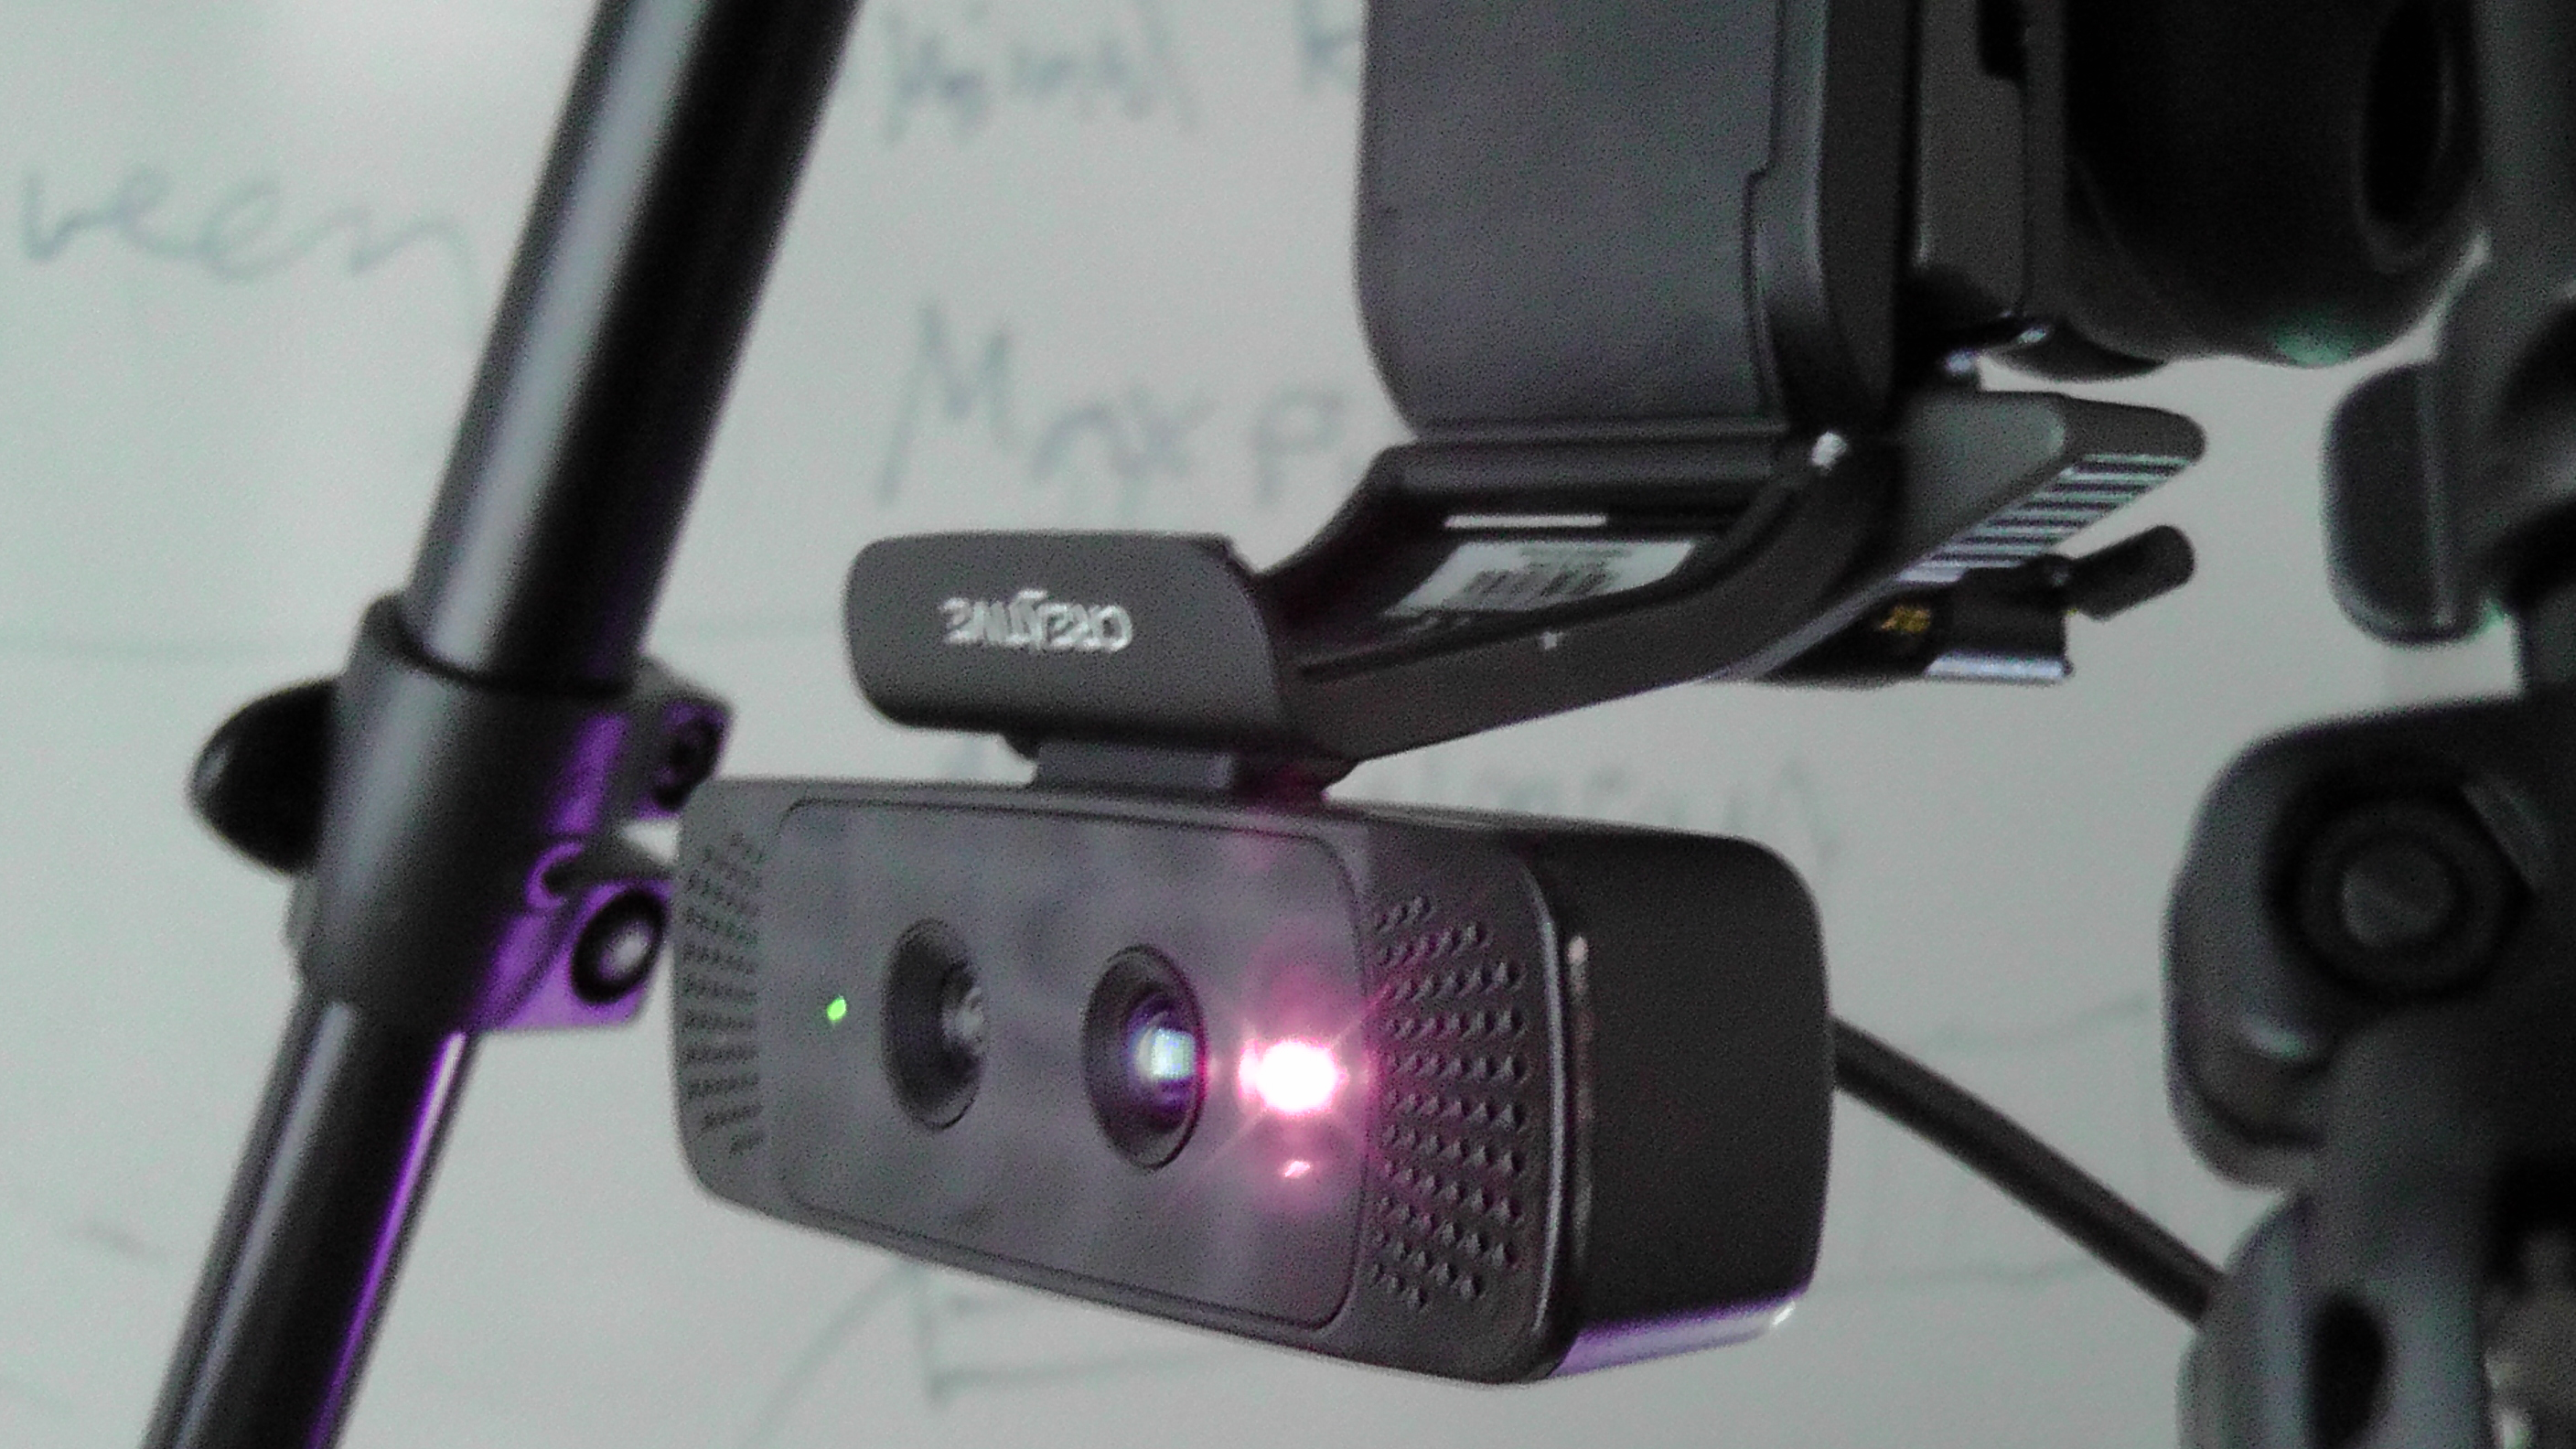
\includegraphics[width=0.6\textwidth]{figures/CreativeDepthCam.JPG}
    \caption{Creative Senz3D Time-Of-Flight(TOF) Depth Camera, mounted on a tripod.}
    \label{fig:CreativeSenz3D}
\end{figure}

In \cite{gokturk}, the authors describe the TOF technology, and state that devices that use it are enabled to perceived and interact with the world around them. Further, the technology is succinctly described as sending out a signal(in this case, light) and measuring a property of the signal(phase shift - differences between sinusoidal wave patterns) that returns from a target. This property can be used to obtain the time of flight. By multiplying it with the velocity of the signal, one can obtain the traveled distance. Lastly, they mention some issues with noise and state that their behavior depends on the amount of light reflected into the sensor.
\end{itemize}


Moreover, a computer was used in order to process the data from the depth camera, project the images onto the display and compensate for the distortion. The computer is a laptop, namely the \textit{ASUS N550JV}. This is included here, to keep in mind when looking at some performance results. The technical specifications can be found on-line.

Finally, a \textit{Manfrotto 190XPROB} tripod was used to mount the camera, so that it does not interfere with the projection, while still being placed fairly close to the screen, around 65cm(it is possible to place it closer, however, if the color stream is needed later on; it is important to check that it covers the full display as well). This tripod is very versatile - one can reverse the column, place it horizontally or even bring down the camera to a height of around 8cm, by using its adjustable legs(if enough room is available).

\begin{figure}[hbtp]
    \centering
    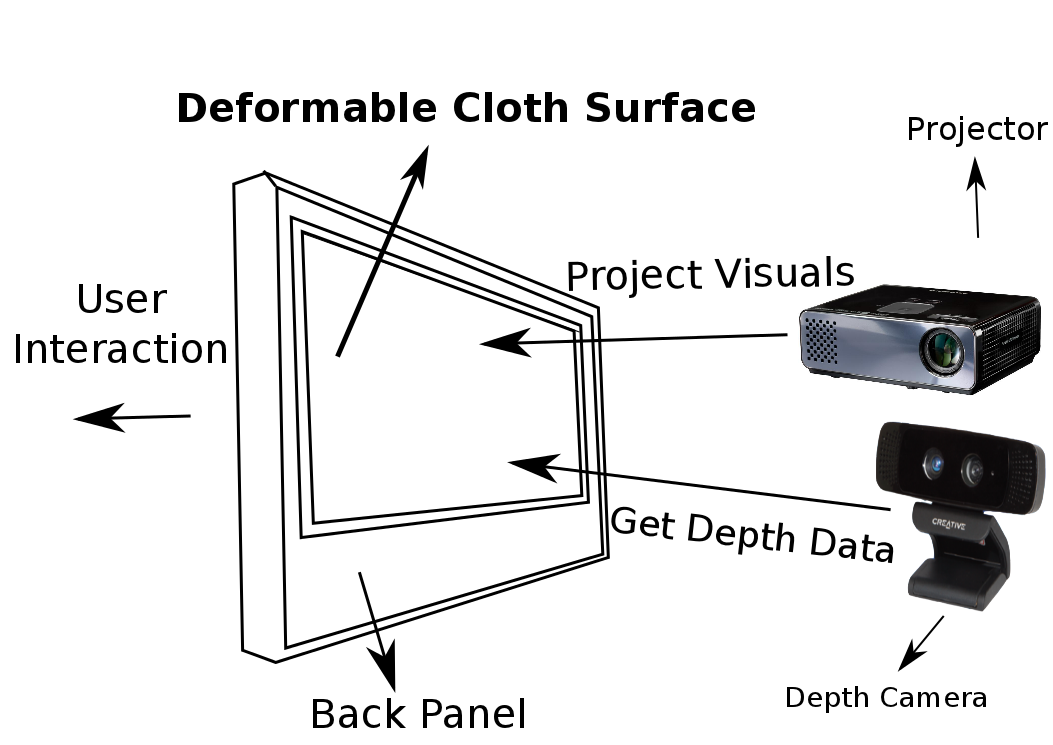
\includegraphics[width=0.8\textwidth]{figures/thesis_setup_illustration_ui.png}
    \caption{Physical setup of the prototype}
    \label{fig:hardware_setup}
\end{figure}

\newpage
\section{Related Work}

In this chapter, relevant research and related works are highlighted, mainly in relation to deformable user interfaces, tracking and projection techniques on deformable surfaces. Investigating related research will help in finding solutions to projection issues with deformable surfaces. Moreover, this will also be useful in order to analyze, compare and contrast different approaches to tracking as well as correcting the projection distortion. 

\subsection{Projection and Tracking on Deformable Surfaces}

\subsubsection{Projection on Non-Planar Surfaces}
As a starting point, it makes sense to consider existing approaches of projection onto complex or non-planar physical shapes. As discussed in \cite{daalsgard11}, calibration is needed in order to correct distortions arising from a difference between the digital and the physical object. The study deals with projection on several physical objects, including a complex, organic, non-planar shape, \textbf{Holger the Dane}, as shown in figure \ref{fig:holger}.

\begin{figure}[hbtp]
    \centering
    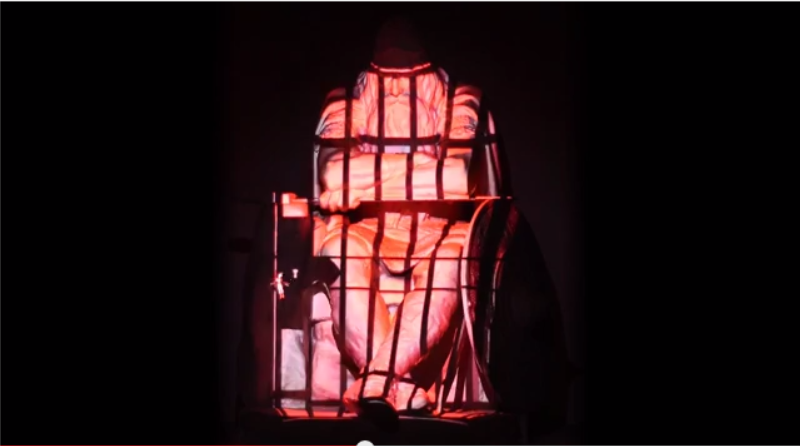
\includegraphics[width=0.8\textwidth]{figures/HolgerTheDane.PNG}
    \caption{Projection on Holger the Dane. Courtesy of \cite{daalsgard11}}
    \label{fig:holger}
\end{figure}

Further, it also proposes a few design themes for 3D projection on physical objects:
\begin{itemize}
\item New potentials for well-known 3D effects (lightning, particle systems, shadows, sound etc…).
\item Dynamics between the digital and physical world and switching between 2D and 3D projections allow to focus the projection on hotspots, while customizing properties allows outlines and switching material textures.
\item Relations between object, content and context.
\end{itemize}

Although the information about the necessity of device calibration, as well as the projection on a complex surface, provide some insights into the projection distortion issue at hand, the study was only concerned with projection on static objects. Thus, it does not address problems arising from dynamic surface deformation, where the projection would need to be adapted in real-time, according to the deformable surface's depth information.\\

Next, \textbf{DeforMe} is a projection-based mixed reality (MR) technique, which provides a method for augmenting deformable surfaces with deformation rendering graphics, as described in [4]. Projected graphics are realistically deformed to match the deformed surfaces. Mixed reality creates the illusion of a virtual modification of the physical surfaces. In this study, a flexible surface is used to allow the user to interact with the projected graphics while obtaining tactile feedback. To summarize, DeforMe is a projection-based MR system which allows projected graphics to be deformed to the deformation of the real object. Various deformable materials can be used without prior knowledge of their mechanical properties or deformation models. However, the aim here is to make the graphics adapt realistically to the surface deformation, while the objective in our current project is to correct all deformations, so that the image looks like on a flat display.

\subsubsection{Tracking Techniques on Deformable Objects}

 In the \textbf{DeforMe} project, the authors present some drawbacks of existing tracking methods such as measuring surface deformation via a depth camera, which is not applicable to tangential deformations that can appear on a surface in a horizontal direction during interactions (e.g.: touching, pulling, etc.). However, we are not interested to model the deformations of the shape realistically, but to correct them, meaning that a depth sensor is adequate to capture the deformation.\\

%However, since depth information can be measured for a cloth-based deformable display (with the material properties being known), it is unclear if there is an %immediate advantage of this method, for the current project, over the tracking techniques employed in the FlexPad system.\\

\textbf{FlexPad}(see \cite{steimle13}), is a real-time interactive system with a highly deformable hand-held paper display. A projector is used to display the visuals, while tracking the display surface with a depth camera provides the required depth information for detecting changes in the surface. Further, as described in the paper, any 2D image from Microsoft Windows can be projected and correctly warped unto the display. 


%\begin{figure}[hbtp]
%    \centering
%    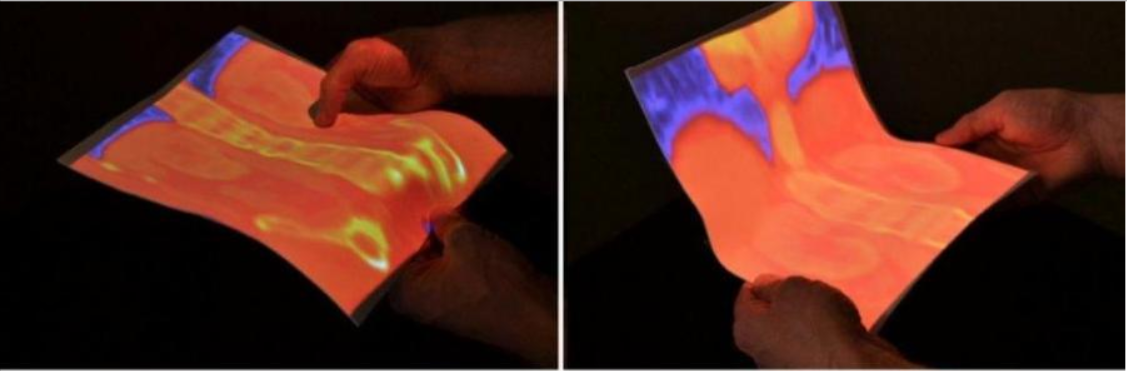
\includegraphics[width=0.8\textwidth]{figures/Flexpad.PNG}
%    \caption{Interaction with Flexpad. Courtesy of \cite{steimle13}}
%    \label{fig:flexpad}
%\end{figure}

Moreover, a deformation model(figure \ref{fig:flexpad_deformation}) is described, in their case using a 25 x 25 vertex plane at the size of the surface. The model can be represented by a 15 dimensional vector consisting of the angles of 8 basic deformations, a z mapping parameter as well as 6 variables for DOF (degrees of freedom) required for affine 3D transformations. 

\begin{figure}[hbtp]
    \centering
    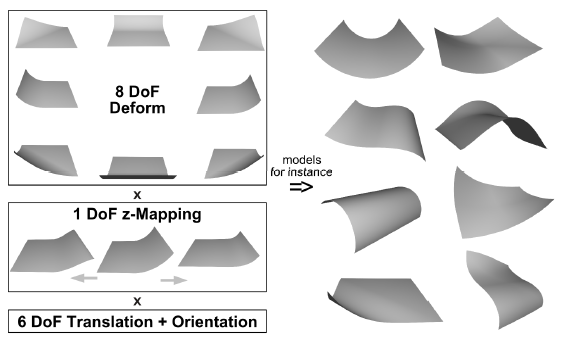
\includegraphics[width=0.8\textwidth]{figures/FlexpadDeformationModel.PNG}
    \caption{Deformation model of Flexpad(left) and deformations it can express(right). Courtesy of \cite{steimle13}}
    \label{fig:flexpad_deformation}
\end{figure}


After obtaining a deformation model, the tracking problem can be defined as finding parameters of the model such that, when synthesized as a depth image, they match the input depth image best(Analysis by Synthesis or AbS). This represents an optimization problem of finding the best parameter vector. More information about this tracking method is available in \cite{steimle13}.

The primary limitations of the FlexPad come from those of the Kinect depth camera not being able to track very sharp bends, however these limitations could be overcome by installing several depth sensors or a more powerful sensor. The hand occlusion issue is not particularly relevant to the current project, since the depth camera was installed in the back of the display, while interaction was done from the front - thus completely removing this problem.

As discussed in \cite{jordt12}, the deformation model can use NURBS surfaces, which can be easily handled via 3D control points, while being able to approximate every surface with arbitrary accuracy. These are widely used in computer graphics and can reduce the high dimensional space of all possible triangle mesh deformations(only the 25x25 vertex plane is used).

The first step is to create an arbitrary NURBS surface using control points and knot vectors, using the algorithm discussed in \cite{jordt12}. Next, once we have an initial triangle mesh(which can be supplied from a modeling program or computed via OpenGL, by reconstructing the object in a static video frame), we can approximate the mesh with a NURBS surface. The NURBS functions must be fitted to the mesh by minimizing the distance between the surface face function and the vertices of the mesh, or, in other words, finding control points for a given set of vertices, that minimize the sum over all squared distances. Mesh registration can then be performed by associating each 3D vertex coordinate to the previously generated NURBS surface. After this step, the mesh can be translated, rotated and deformed by displacing the control points of the NURBS surface function.\\

An alternative to this tracking method is employed in \cite{watanabe08}. Moreover, deformation correction is also implemented, in the previously mentioned paper. Therefore, it is described in the following section.


\subsection{Distortion Correction on Deformable Surfaces}

Another project that provides useful information on projecting onto irregular 3D surfaces, as well as tracking them using depth data, is \textbf{The Office of the Future}(see \cite{raskar98}). One of their objectives is to use real surfaces in the office, as spatially immersive display surfaces. High-resolution graphics is projected onto these surfaces(see figure \ref{fig:future_office}).

\begin{figure}[hbtp]
    \centering
    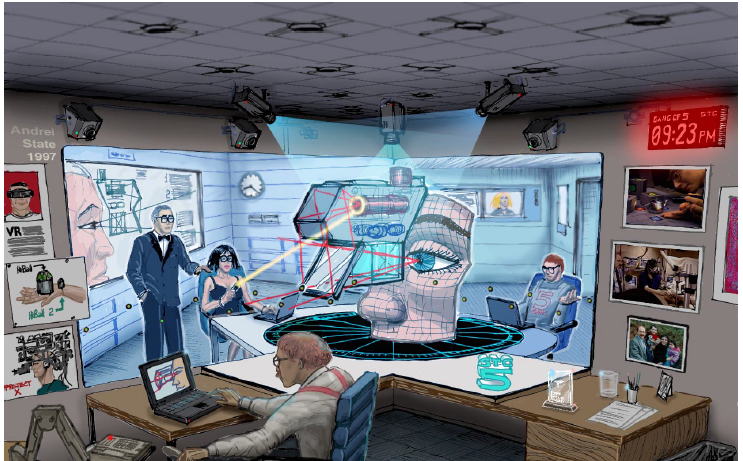
\includegraphics[width=0.8\textwidth]{figures/FutureOffice.PNG}
    \caption{The Future Office. Courtesy of \cite{raskar98}}
    \label{fig:future_office}
\end{figure}

They extract depth using imperceptible structured light (projecting binary-coded patterns that are not detected by the visible eye and recording the images with video cameras) - this process can be replaced in the current project by the use of an off-the-shelf depth camera. Further, they describe how, by knowing the object's surface, the viewer's location, projector calibration parameters and the contents to be projected, they can render on irregular 3D surfaces by the use of conventional 3-D methods(e.g.: \textbf{PTM}(projective texture mapping)), in real-time. Finally, they state that their system can be used to detect display surface changes at non-interactive rates. However, due to a large increase in computing power in recent years, and the possibility to write custom graphics programs that run directly on the hardware(e.g.: shader programs), similar techniques can be used today, to detect display surface changes in real-time.\\

\textbf{The Deformable Workspace}(see figure \ref{fig:deformable_workspace}) is another approach to creating a deformable screen that acts as a boundary surface between the real and virtual worlds and is presented in [5]. The workspace is set up in similar ways to other techniques by using an IR camera, IR projector and an LCD projector. Basically, the IR camera and projector could be replaced by a depth sensor such as the Kinect. 

\begin{figure}[hbtp]
    \centering
    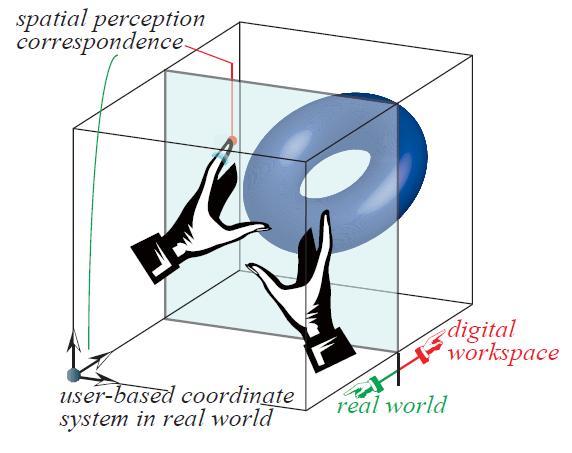
\includegraphics[width=0.8\textwidth]{figures/TheDeformableWorkspace.PNG}
    \caption{The Deformable Workspace Setup. Courtesy of \cite{watanabe08}}
    \label{fig:deformable_workspace}
\end{figure}

Tracking is based on triangulation using structured light. A single snapshot of the illuminated surfaces is sufficient to grasp complete screen deformation - a high-speed camera acquires the image, and a dedicated co-processor for high-speed image processing calculates the coordinates of a 3D point for each spot of light in the pattern (real-time performance at 955fps with a latency of 4.5ms), as described in \cite{watanabe07}. Although the frame rate achieved is incredibly high, this is a custom solution, that requires separate hardware. The previous method shall not be employed for this project as the deformable display can now be tracked with a standard depth camera(either a structured light or time-of-flight depth camera).

In [5] they also provide a method to compensate for projection distortion, given that both the calibration parameters and the shape of the deformed screen are known. The technique involves pre-warping the image by shifting each projected point. Further, they claim that PTM can be used to calculate and render the warped image to be projected in real-time, efficiently and easily. A limitation of the previous approach is that an assumption has been made that the user’s eyes are fixed. However, a viewpoint-based projection should be employed to accommodate realistic scenarios - the virtual space must be rotated and transformed according to the change of viewpoint.\\

Perhaps another solution, would be to use some kind of spatial distortion, similar to the approach used for the \textbf{JellyLens} (see \cite{pindat12}). The focus + context lens(uses two levels of detail to connect a magnified region to the selected context)  can dynamically adapt to the shape of the objects of interest. As we can see in figure  \ref{fig:JellyLens}, the object of interest adapts its shape(is magnified), while the context is preserved - surrounding objects are almost untouched by the applied distortion.

\begin{figure}[hbtp]
    \centering
    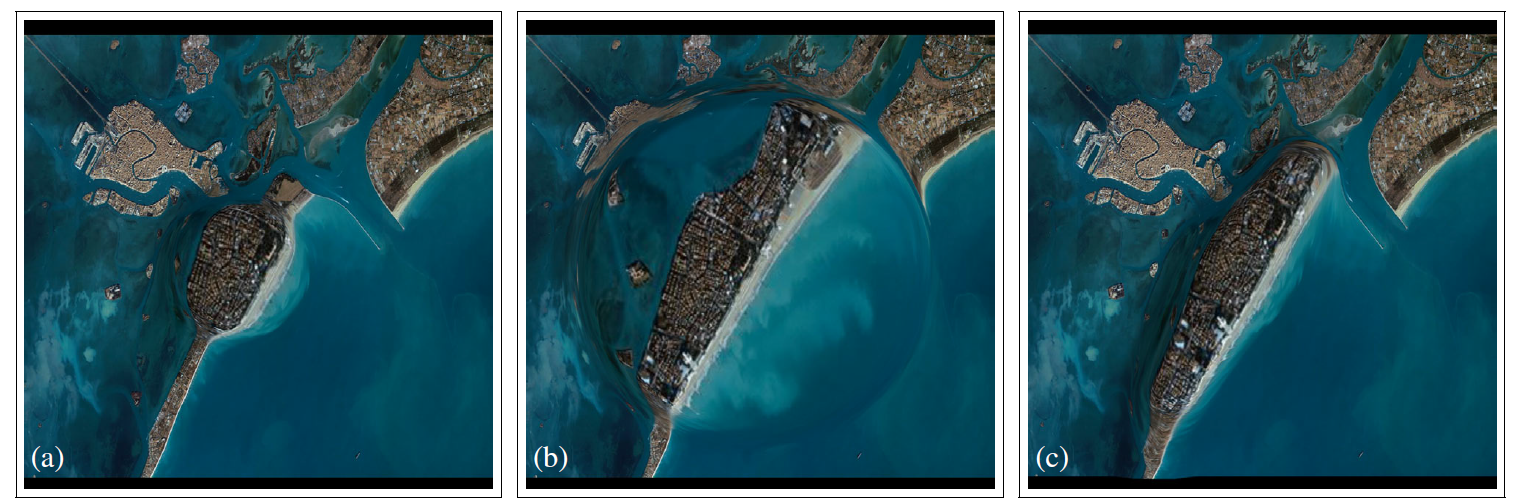
\includegraphics[width=0.8\textwidth]{figures/JellyLens.PNG}
    \caption{a) Only a portion of the object can be magnified with a small fisheye lens; b) A large fisheye magnifies almost the entire object, but at the cost of added distortion for surrounding objects; c) JellyLens - adapting the relevant information of the object, while preserving the surrounding areas. Courtesy of \cite{pindat12}}
    \label{fig:JellyLens}
\end{figure}

The JellyLens can adapt to match the geometry in a three-step process:
\begin{itemize}
\item Obtaining information about the geometry of the objects (in our case, this can be accomplished by transforming our object depth data to 3D geometry)
\item Computing the lens shape according to its position and visualization and to the geometry of the nearby objects of interest (in our case, the depth data can be used to determine how to shape the lens)
\item Rendering of the region seen through the lens (in our case, we can apply a normal texture on the deformable mesh's geometry - that represents the contents, and distort it according to the lens shape obtained previously)
\end{itemize}

The authors of \cite{pindat12} also describe in detail how to model and adapt the lens using two techniques known as \textit{AreaLens} and \textit{PathLens}. For more detail about the process, please consult this reference.\\

\subsection{Chapter Summary}

This review has highlighted some of the main methods of projecting, tracking and correcting distortions for non-planar deformable objects. Further , we could observe that the techniques used to project onto irregular objects and to correct the visuals, are similar in \cite{watanabe08} and \cite{raskar98}: both extract depth information and form a polygonal model of the target object, they use the same rendering technique(PTM) and require the same calibration parameters. Moreover, the NURBS deformation model used in \cite{steimle13}, could be employed as an alternative to the methods described in the two previously mentioned sources.

The existing work on this topic helped to identify the main steps that are required in order to compensate an image and correct it's distortion. Information about alternatives to some of these steps has also surfaced. This literature review has guided my choices through the remaining chapters.

\newpage
\section{Prototype Design and Theoretical Considerations}

Both the projector and the depth camera were fixed in place relative to the deformable screen. Further, the projected visuals would normally be interactive applications for such a display - they need to be rendered continuously. Finally, due to the fact that the projected image was warped (distorted) according to the screen deformation, an algorithm was needed to shift the projected image pixels corresponding to the display surface’s depth data. 

\begin{figure}[hbtp]
    \centering
    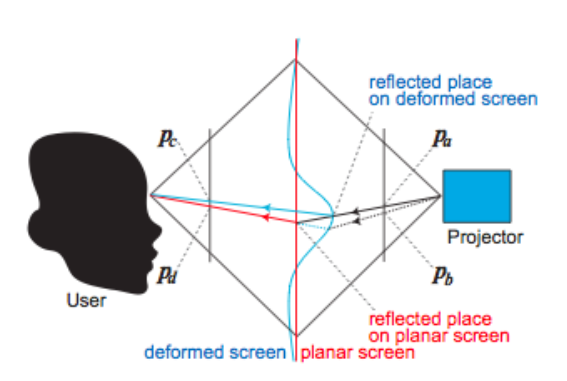
\includegraphics[width=0.8\textwidth]{figures/PointProjection.PNG}
    \caption{Compensation of image warp caused by screen deformation. Courtesy of \cite{watanabe08}}
    \label{fig:PointCompensation}
\end{figure}

In figure \ref{fig:PointCompensation}, $p_{d}$ is the position where the ray is observed for a planar screen, while $p_{c}$ is that of the deformed screen, if the projection is from $p_{a}$. To observe $p_{d}$ for the deformed screen, projection must be from point $p_{b}$. Consequently, the image point needs to be translated to this position, in order to compensate for the distortion.\\

A possible approach to solving the distortion issue is discussed in \cite{watanabe08}, where the authors state that in order to compensate for the distortions of the display one needs to know the shape of the deformed screen (depth data) and the projector calibration parameters. \\

For this project, a solution similar to that employed in \cite{watanabe08} has been implemented. This is because it was the only paper where distortion correction in a 3D space was more thoroughly addressed, thus reducing risk. Further, similar techniques could be easily used with our hardware setup. It was unclear whether the other methods, such as the NURBS model used in \cite{steimle13} would be accurate enough for compensation - the deformation model is approximated; if the offset is too large, deformations may not look right.

In order to get a better overview and understanding of the whole process required to correct the distortions, I have created a system pipeline(see figure \ref{fig:Pipeline}) that describes the whole process, at a high-level. Each part will be described individually in subsequent chapters.

\begin{figure}[hbtp]
    \centering
    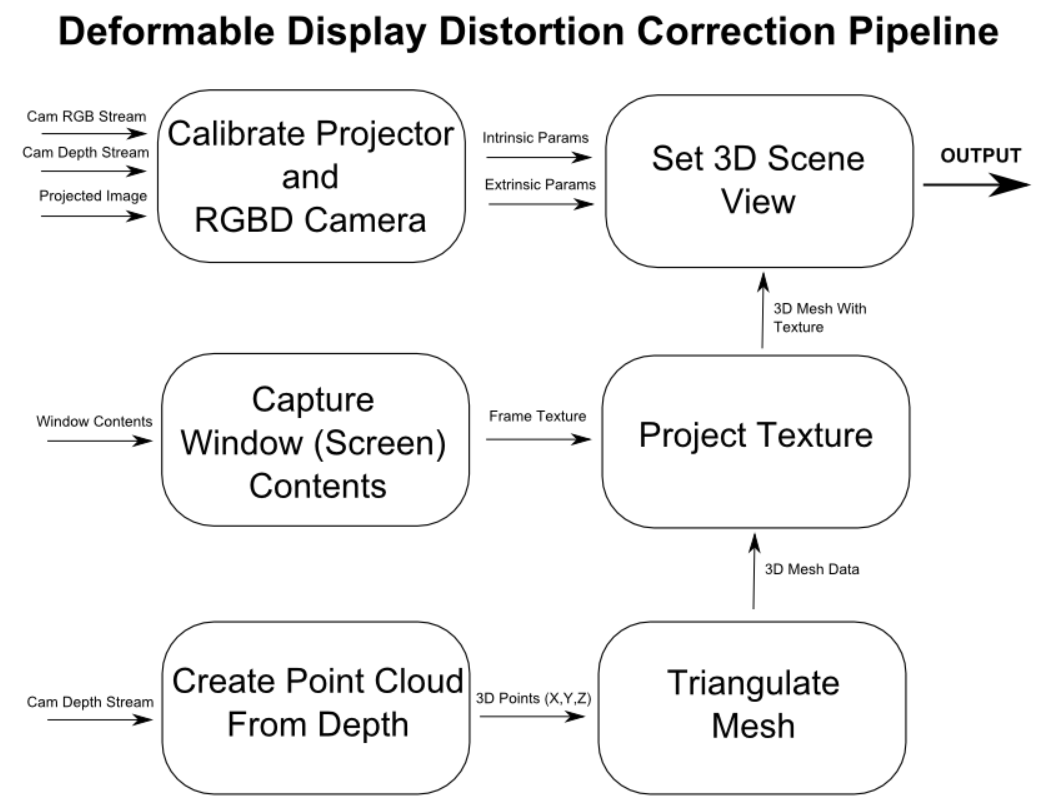
\includegraphics[width=0.8\textwidth]{figures/DeformableDisplayPipeline.PNG}
    \caption{Distortion Correction Pipeline}
    \label{fig:Pipeline}
\end{figure}
\newpage
\subsection{System's Pipeline Overview}

Considering our system pipeline, I will explain briefly, how the whole components work and why they are needed, in this section. The first process is calibration. Note that the order in which components are explained does not represent the flow in the pipeline, since it will be easier to see, for example, why calibration is needed once some of the other steps have been explained.\\

The idea followed in \cite{watanabe08} consists of displaying the final application contents on a 3D model representation of the deformable surface. In order to obtain a relatively stable model, one can convert the depth data into a 3D mesh. An intermediary step required in order to do so, is to first create a point cloud from the depth data, or in other words, to use the depth value as the z-coordinate and create a cloud of points with coordinates $(X, Y, Z)$ corresponding to the image pixels and depth.\\

Further, the application contents must be displayed in such a way that they distort with the object. Like with most problems in computer graphics, there is more than one solution. One could, for example, use raytracing to directly project rays of light on the object(also mentioned by the authors of \cite{raskar98}). However, this approach is known to be slow and may not run in real-time. Alternatively, there exists a technique which is known in computer graphics, which projects a texture onto an object as from a slide projector(PTM). This technique can also be implemented in real-time on modern hardware. Further, since the texture is projected from a virtual projector in the 3D scene, it will update with the distortions corresponding to the deformation on the object.\\

Finally, we need to make sure that our virtual camera corresponds, as closely as possible to the area we project onto with our physical display. Further, we also need to place our virtual projector, which requires information about where the mesh(3D model) is placed, and how it is oriented. In addition to position and orientation we must also know the field of view(FOV), or the \textit{"zoom level"} of our camera(as the other parameters depend on the FOV). In addition to the calibration required above, one also needs to manually(physically) align the projector so that if correctly fills the deformable display area. Furthermore, in case of manual calibration, the depth camera must also be placed as orthogonal as possible to the deformable surface area, so that it is easy to obtain acceptable parameters for the virtual camera and projector described above. At this point, we basically have a solution to the distortion correction problem. The only remaining issue is to update the application contents dynamically, by capturing window/screen contents. This can be accomplished by using textures. In the next sections, each of the above will be described in greater detail.

\subsection{Calibration of the Projector and the Depth Camera}

In order to properly display the contents on the deformable surface, three things must be ensured:
\begin{itemize}
\item The projector must be calibrated in order to find the intrinsic and extrinsic parameters that will be used to compute a transformation matrix that defines the world view of the 3D scene
\item The physical projector must be aligned with the deformable screen area. Further, the depth stream must be adjusted manually so that the deformable display is almost perfectly in view, if the calibration is done manually, by trial and error; 
\item The projector and camera are static and must not be moved, otherwise the calibration process has to be repeated\\
\end{itemize}

The calibration problem is a projector-camera calibration problem, similar to the illustration shown in figure \ref{fig:ProjectorCameraSetup}. The only difference being that, for this project, an RGBD camera(RGB stream + depth stream) is used. This means that there are two cameras: a normal RGB video camera, and a depth camera. If the calibration is done between the RGB camera and the projector, the RGB camera must then be correctly mapped to the depth camera or vice-versa.

\begin{figure}[hbtp]
    \centering
    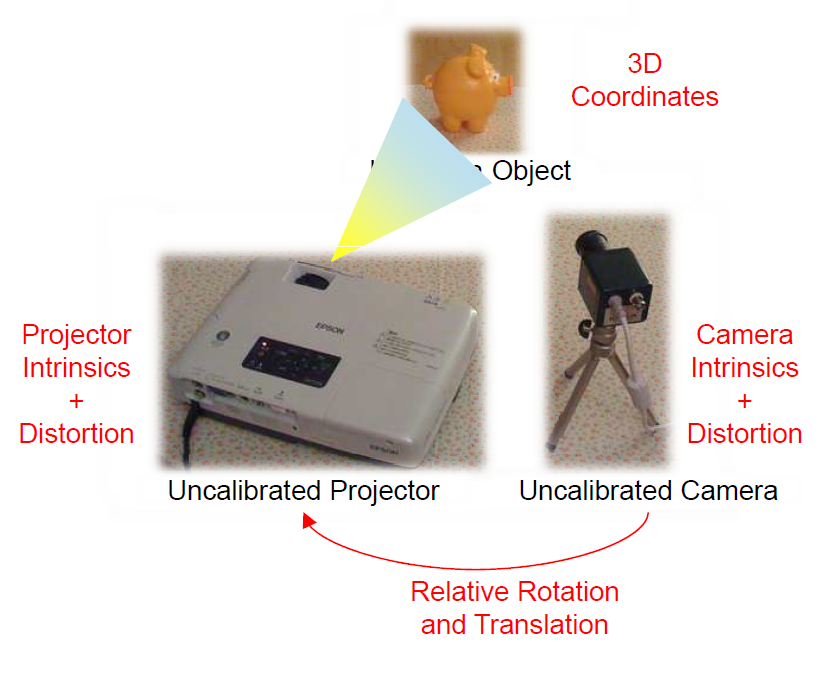
\includegraphics[width=0.8\textwidth]{figures/Projector-Camera_Calibration.PNG}
    \caption{A setup that needs projector-camera calibration}
    \label{fig:ProjectorCameraSetup}
\end{figure}

In order to properly align the physical projector/camera with the virtual projector/camera we need to compute two matrices in a virtual world, based on parameters extracted from the calibration procedure. The first is the projection matrix, which can be represented as a frustum(see figure \ref{fig:Frustum}). We can define the projection matrix in OpenGL either by providing all the frustum parameters(the near and far parameters can be entered manually), or a field of view and aspect ratio, from which they can be computed. 
\begin{figure}[hbtp]
    \centering
    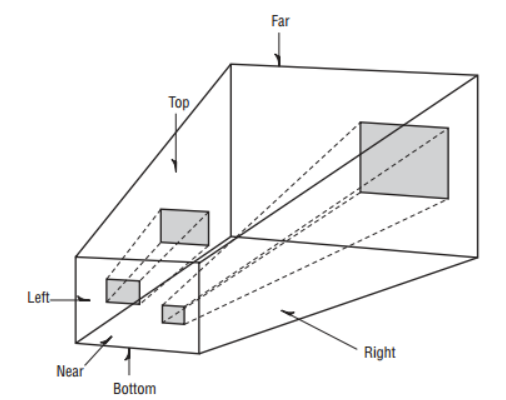
\includegraphics[width=0.8\textwidth]{figures/Frustum.PNG}
    \caption{The projection frustum. Courtesy of \cite{superbible}}
    \label{fig:Frustum}
\end{figure}

It essentially defines the viewing volume of our 3D scene. In order to compute this matrix, one needs to know the intrinsic parameters of the physical projector.
\textbf{Intrinsic parameters} refer to different aspects of a camera/projector such as focal length, scale parameters, a tilt compensation parameter and the image coordinates which define the image center or principal point. In addition, other parameters can be included to account for lens distortion. Lens distortion will not be addressed in the current project. The images projected with a modern device have low distortion.\\

Secondly, we need to compute the modelview matrix(see figure \ref{fig:MVMatrix}, for the structure of such a matrix). This matrix has information that relates to the position of the 3D object(model) as well as the camera(eye space). In this case, we essentially need to compute the view matrix from the extrinsic parameters, so that our virtual camera correctly points to the deformable display area on which our target contents are projected. \textbf{Extrinsic parameters} represent the \textbf{location} and the \textbf{orientation} of the projector/camera with respect to a world reference frame. For example, if we choose the world origin to be the position of the depth camera, then we can compute the rotation and translation of the projector with respect to the depth camera by finding the rotation matrix R and translation coefficients T. To obtain camera coordinates from world coordinates we simply need to multiply a position by R and add the translation T.

\begin{figure}[hbtp]
    \centering
    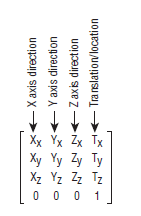
\includegraphics[width=0.4\textwidth]{figures/MVMatrixOGLSB.PNG}
    \caption{A 4x4 matrix that represents a position(column 4) and orientation(columns 1-3) in space. Courtesy of \cite{superbible}}
    \label{fig:MVMatrix}
\end{figure}

The pinhole camera model can be used to represent the projector, only the direction of the light rays are opposite, so the projector is in fact, an inverse camera model. The general pinhole camera model, where the center of projection does NOT have to be the world coordinate system is shown in figure \ref{fig:PinholeCameraModel}.

\begin{figure}[hbtp]
    \centering
    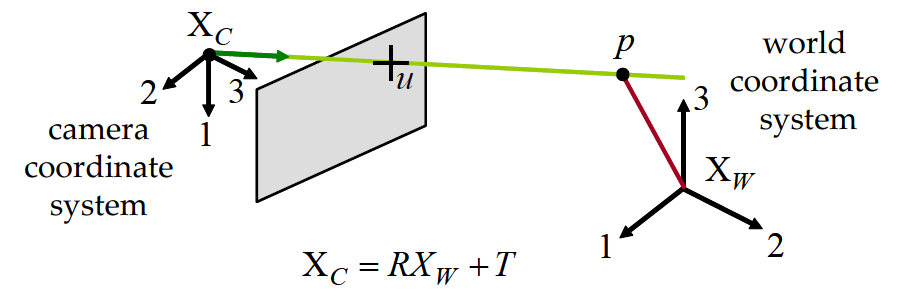
\includegraphics[width=0.8\textwidth]{figures/GeneralPinholeModel.PNG}
    \caption{General Pinhole Camera Model}
    \label{fig:PinholeCameraModel}
\end{figure}
\newpage
\subsubsection{Approaches to Calibration}

\begin{itemize}
\item Structured Light Illumination Patterns
\\
\\The correspondences between 2D pixels and 3D world coordinates are found in both \cite{radhwan11} and \cite{yamazaki11} by employing the structured lighting approach which involves projecting gray coded patterns that represent projector rows/columns onto the surface. This approach requires a camera to capture the projected patterns.

An advantage of this approach is that it does not require any other physical items (such as printed checkerboard patterns), neither moving objects around, for calibration. However, it does require depth information, as it does not work well with planar objects. This information is almost absent in our case, because the display is almost flat in it's initial state. Even though the parameters could be retrieved by using this method, the final results were never satisfactory(even when using cardboard boxes for generating depth data).\\
\item Checkerboard Pattern\\
\\Another approach for calibrating a projector-camera system is to use printed checkerboard patterns, extending from Zhang's method, as discussed in Chapter 3 of \cite{lanman09}. The known checkerboard patterns are projected onto a diffuse rigid object and their distorted appearance is photographed. Since a projector is the inverse of a camera, points on the image plane are mapped to outgoing light rays that pass through the center of projection. About 10-20 images with different positions and pose should be recorded.

In \cite{falcao08} a plane-based calibration of a projector-camera system is described. It can be used to obtain the intrinsic and extrinsic parameters of both the camera and the projector. The steps involved are:
\begin{itemize}
\item Calibrate the camera using Zhang's method
\item Recover calibration plane in camera coordinate system
\item Project a checkerboard on calibration board and detect corners
\item Apply ray-plane intersection to recover 3D position for each projected corner
\item Calibrate the projector using the correspondences between the 2D points of the image that is projected and the 3D projected points
\end{itemize}


The procamlib (https://code.google.com/p/procamcalib/) software package for Matlab can be used to calibrate the projector-camera system using this approach. The steps are explained in \cite{falcao08}. However, both the projected checkerboard and the printed one need to be in view of the camera at the same time. This is not possible with the setup used in this project.\\
\item 3D Projection Mapping by Using a Reconstructed 3D Object\\

The calibration approach described in \cite{vvvv} used a reconstructed 3D scene in order to calibrate the projector. Several vertices are selected on the reconstruction, to be used as calibration points. These can be selected as to correspond to the area where we are projecting. This technique could not be used, since a fully shaded reconstruction of the deformable cloth was not available for use. At this time, I could not find reconstruction tools for the \textit{Creative Senz3D} camera(the authors of this approach use the \textit{Microsoft Kinect}). However, some attempts were made to save the mesh in an \textit{.obj} file. However, this was not completed due to lack of time(some faces were connected in a wrong order) and mesh normals would also have to be computed to shade the cloth(so that we are able to see the cloth area in the calibration package, where we would need to place our calibration points).
\item openFrameworks Camera-Projector Calibration\\

A software package that calibrates a camera and a projector is available as an \textit{openFrameworks}(a toolkit for C++ applications) addon. The method is demonstrated in a video(see \cite{ofx}). It should be mentioned that this addon has originally been developed by one of the authors of \cite{watanabe08} and later extended. I had some trouble running the code, but after I made some changes it seemed that I successfully calibrated the camera+projector, since, as in the video, the projected dots were correctly rendered, when rotating and moving the checkerboard. However, the output for the rotation part of the extrinsic parameters was only a vector. In OpenGL I needed a rotation matrix. The matrix can be retrieved by using what is known as the \textit{Rodrigues' rotation formula}. I have used a readily available Matlab function that supposedly did the conversion. This was used like a black-box, I did not study how the formula works, as I was short on time. 

Further more, if the values are calculated using OpenCV's coordinate system, we have to change it to OpenGL's reference sytem by a 180 degree rotation around the X-axis, due to the differences shown in figure \ref{fig:OpenCVOpenGLCoords}. 

\begin{figure}[!hbtp]
\centering
\begin{subfigure}{.5\textwidth}
  \centering
  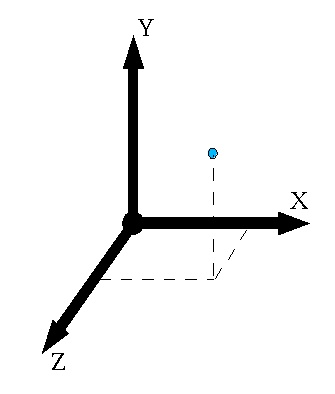
\includegraphics[width=0.9\linewidth]{figures/OpenGLCoords.jpg}
  \caption{OpenGL}
  \label{fig:OpenGLCoordinateSystem}
\end{subfigure}%
\begin{subfigure}{.5\textwidth}
  \centering
  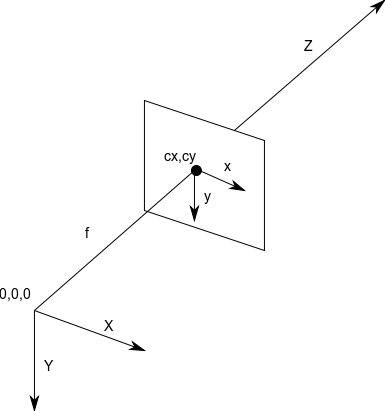
\includegraphics[width=0.9\linewidth]{figures/OpenCVCoords.png}
  \caption{OpenCV}
  \label{fig:OpenCVCoordinateSystem}
\end{subfigure}
\caption{Coordinate system differences between the two libraries.}
\label{fig:OpenCVOpenGLCoords}
\end{figure}

Moreover, as mentioned in an on-line article(see \cite{vuforia}) the pose matrix (effectively the matrix that combines both rotation and translation parameters), is what one could use to draw a virtual object at the target camera location, but, in order to tell how the camera is placed with respect to the target(which is what we need in this case, since the target is the deformable display, and we want to find the camera view which corresponds to the cloth area), the matrix needs to be inverted. These steps have been applied, but the mesh was scaled non-uniformly(skewed) when using the rotation matrix obtained previously. I did not find out why this was the case, and a manual alignment of physical and virtual cameras has been used instead. 

As a final note, the coordinates of the mesh points were computed from the depth data and they would need to be mapped to the color coordinates, or the pose matrix has to be converted so that the calibration is between the depth camera and the projector, not the color camera. The calibration values for both depth and RGB cameras can be obtained from the Intel Perceptual Computing SDK.

\item Manual Adjustment\\
\\It is also possible to adjust the physical projector and camera so that one can compute the extrinsic parameters, provided that the intrinsic parameters are known. The latter may also be obtained by looking into the respective product's datasheet and adjusting the value depending on distance, lens size etc, or computed by a trial and error approach. As the trial and error approach was used in this project, some tests need to be done to confirm that the accuracy is acceptable. Manual adjustment is likely to produce results of inferior quality, compared to the previously mentioned methods.
\end{itemize}

\subsection{Creating a Point Cloud from the Depth Data}

This step is an intermediary one towards creating a mesh structure on which textures can be projected. A 3D point cloud is a set of data points in the third dimension, usually defined by $(X, Y, Z)$ coordinates.

The depth camera retrieves an image of 320x240 depth pixels. A point cloud can be created by using x, y values from 0 to the width and height of the depth image, respectively. The z value is simply equal to the depth, if the depth value is in a certain range(after it has been filtered). If the depth value is invalid, the current point is discarded and will not be rendered.

Further, the point cloud must be updated in real-time. Rendering is being done with OpenGL, and the previous can be accomplished by using simple hardware graphics shader programs and OpenGL's Vertex Buffer Objects(VBO). The OpenGL point cloud also has to be rotated, as it is upside down - unless the depth camera is positioned upside down, which it was in the final setup.

In the following, I will include a section with information about the general rendering process, which is used to render 3D objects with the programmable OpenGL pipeline. The process is similar whether we wish to render a point cloud, or a 3D mesh - only the vertex attributes(position, color, texture coordinates, normals etc.) which are stored in the VBOs and the programmable shaders will change.

\subsubsection{Rendering}

The transformation pipeline(see figure \ref{fig:TransformationPipeline}) describes how the vertex information is transformed from raw data, to window coordinates that can be viewed on a screen. The raw vertices are first multiplied by the modelview matrix, which yields the transformed eye(view) coordinates. Then, we multiply the result by the projection matrix and obtain clip coordinates. All data outside the clipping space(frustum) is removed. Then, coordinates are divided by the $w$ value to yield normalized device coordinates  in the +/-1.0 range, for all axes. Finally, OpenGL internally maps the scene to a 2D plane by the viewport transformation matrix, based on the viewport parameters provided.

\begin{figure}[hbtp]
    \centering
    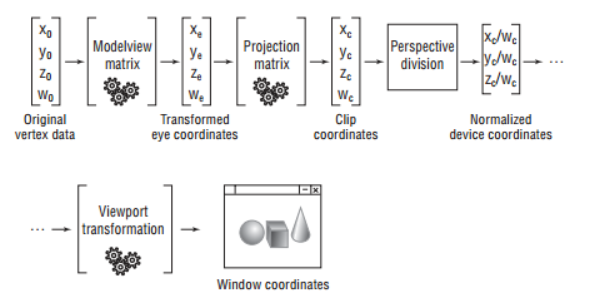
\includegraphics[width=0.8\textwidth]{figures/TransformationPipeline.PNG}
    \caption{Vertex Transformation Pipeline. Courtesy of \cite{superbible}}
    \label{fig:TransformationPipeline}
\end{figure}


In the following, I will briefly describe the 3D graphics pipeline, shown in figure \ref{fig:GraphicsPipeline}. It explains the stages required to process the vertices in order to obtain colored pixels and how vertex attributes can be programmed in the two shader stages(using the vertex and fragment processors).

\begin{figure}[hbtp]
    \centering
    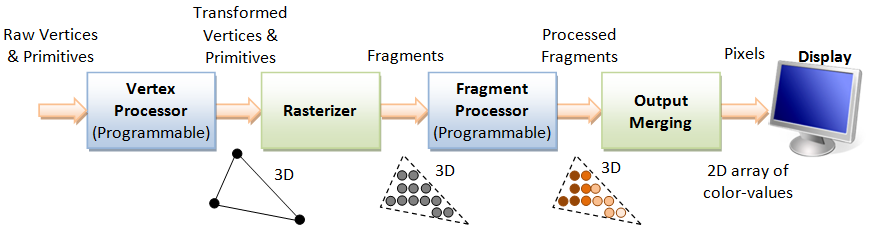
\includegraphics[width=1.0\textwidth]{figures/Graphics3D_Pipe2.png}
    \caption{3D Graphics Pipeline}
    \label{fig:GraphicsPipeline}
\end{figure}

As we can see from the pipeline, the raw vertices are processed by a vertex processor which manipulates vertex related attributes, most generally, position. For example, a vertex shader(a program that runs on this processor) can be used to apply the modelview matrix to an input vertex. Next, the data is rasterized into fragments.
 
A fragment contains the data necessary to generate a single pixel's worth of a drawing primitive in the frame buffer(the frame buffer is a portion of memory that contains a bitmap that will be sent to the video display - it represents a complete frame of data): raster position, depth and, after the fragment shader stage, it also contains interpolated attributes such as color and texture coordinates as well as a stencil value, an alpha value and the window ID. Note that a fragment only corresponds to a pixel if antialiasing is turned off, otherwise there will be $K$ fragments for a pixel for $K$x level antialiasing.
As we can see from the above, the fragment shader receives fragments and processes them, computing color and texture coordinates. This shader can be programmed to color the geometry in any way desired. One can also apply textures and lighting at this stage. Finally, fragment shaders are also useful for visual debugging, as shader programs can usually not be debugged, since they run on the GPU hardware.\\

\subsubsection{Point Cloud Density}

Unfortunately, unless the point cloud is of sub-pixel density(which would also require a lot of processing power, due to the very large number of OpenGL primitives), it is easy to see that the target object is in fact made of discrete points(see figure \ref{fig:PointCloud}). This breaks immersion, especially after applying a texture to the object. Due to this, we must then proceed to the following step, triangulation of the points into a 3D mesh.

\begin{figure}[hbtp]
    \centering
    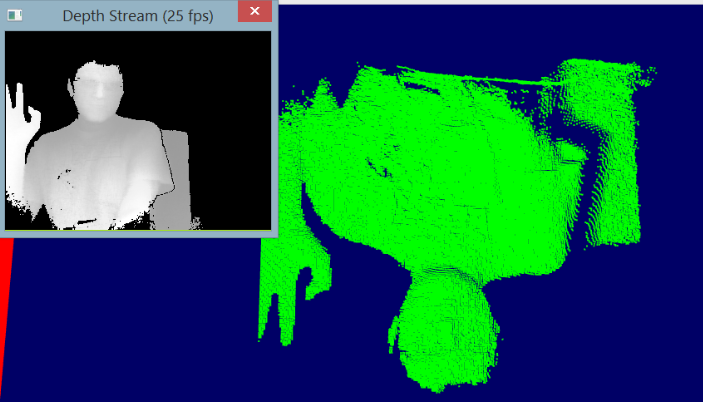
\includegraphics[width=0.8\textwidth]{figures/PointCloud.PNG}
    \caption{An example point cloud, corresponding to the depth stream, updated in real-time.}
    \label{fig:PointCloud}
\end{figure}

\subsubsection{Unprojecting to World Coordinates}
\label{sec:unprojecting}

 Before we proceed to triangulation, we must also unproject the points to world coordinates(we just had pixel positions and depth values, but we need to obtain the coordinates in regular metric space, so that the distances between the points are correct). This operation requires knowledge about intrinsic camera parameters, since we need to know the projection matrix, in order to unproject the points:

$$point => Viewport^{-1} => Projection^{-1} => ModelView^{-1} => PointInWorldSpace$$

More information about the unprojecting process is available in \cite{sung2013}, although the authors unproject a 2D mesh with a set of sparse depth points. Nevertheless, the authors explain that unprojecting is the inverse process of how normal images are obtained, by projecting rays into a camera. In order to compute the rays, one needs to know the focal length and image center(intrinsic parameters), as well as the distance of the unprojection(ray length, which, in our case, corresponds to the depth for that pixel). They explain that the 3D position for a vertex $v(x,y)$ can be denoted by $p(v)$ and is determined as:
$$p(v) = t(v) *\vec{r}(v),$$
where $t(v)$ represents the ray length and $\vec{r}(v)$ represents the ray direction and is equal to $$\vec{r}(v) = (\frac{x - x_{c}}{f},\frac{y-y_{c}}{f},1)^T,$$ where $(x_{c}, y_{c})$ is the principal point or image center and f represents the focal distance.

However, the official library for the depth camera used in this project provides a very useful method that computes the unprojection given the array and number of points. So in the end, that is all we really need to know in order to unproject the points, if we are using the \textit{Creative Senz3D} depth camera.
 
\subsection{Object Reconstruction by Mesh Triangulation}

Before delving into the different methods of object reconstruction, it should be mentioned that there is an alternative to the full reconstruction approach. In \cite{Jordt2011}, a method of tracking deformable objects using depth and color streams is described. The authors of this paper have used a NURBS(Non-uniform rational b-spline - common in computer graphics; can be used to approximate curved surfaces) based deformation function to decouple the geometrical object complexity from the complexity of the deformation. They deform the mesh using a number of control points(low dimensional space when compared to the number of vertices) on the NURBS surface to which the object is mapped. However, it is still needed to have an initial mesh and one way to obtain it is to define a 3D object from the initial frame of the video streams. The desired object can first be segmented out of the frame, and then the 3D vertices can be unprojected to 3D space and connected according to their adjacencies in the depth image(actually, in section \ref{sec:TriangleStripTriangulation} a similar method is used, but it is running on the GPU and updates the mesh every frame). This mesh can be subsequently deformed using the control points, so that it matches the depth and/or color data. The mesh is also mapped to the color image to retrieve the colors of the vertices, but this is not needed for the deformable display, since a texture will be projected onto the mesh, completely replacing any color and lighting information.

Coming back to the general topic of object reconstruction, there are several techniques for reconstructing a 3D mesh from a point cloud. An important aspect for our deformable display is that we only need a 2.5D correct mesh, similar to a terrain(see figure \ref{fig:PerspectiveTerrain}) or heightmap. 

\begin{figure}[hbtp]
    \centering
    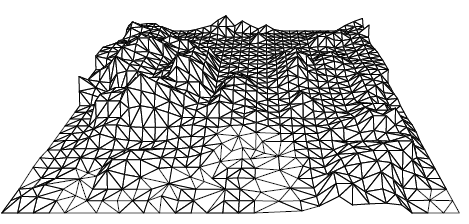
\includegraphics[width=0.4\textwidth]{figures/PerspectiveTerrain.PNG}
    \caption{Perspective View of Some Terrain. Courtesy of \cite[Chapter~9]{berg08}}
    \label{fig:PerspectiveTerrain}
\end{figure}



In order to obtain a full 3D model of an object, we would, anyway, need to rotate the depth camera around the object, or use multiple depth cameras, that look at the object from different angles. We always look from the front of the deformable display, as we would, down on a terrain, so such 3D detail is not needed. Therefore, the most straight-forward, naive approach, is to simply find any triangulation for the point cloud. In order to do this we can consider a grid of points, that can be connected either by using triangles or a triangle strip. The main idea of this method is also shown in figure \ref{fig:PolyhedralTerrain.PNG}, where a terrain is triangulated from some sample points.

\begin{figure}[hbtp]
    \centering
    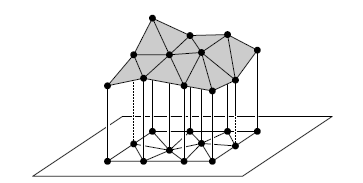
\includegraphics[width=0.4\textwidth]{figures/PolyhedralTerrain.PNG}
    \caption{Polyhedral(solid object with flat surfaces) Terrain. Smoothness will depend on point density. Courtesy of \cite[Chapter~9]{berg08}}
    \label{fig:PolyhedralTerrain.PNG}
\end{figure}

Although the naive approach has been implemented and used in this project, some more sophisticated alternatives will also be described and contrasted, as this approach was not the first one attempted.

\subsubsection{Connect a Grid of Points with a Triangle Strip}
\label{sec:TriangleStripTriangulation}
Since the depth data captured via a depth camera is ordered, the easiest way is to consider the point cloud as a grid of points. Then, one can connect the vertices together using triangle strips. Triangle strip representation is a method of drawing triangles that can save some of the memory bandwidth, by connecting a new triangle to an existing strip with each new point. This means, that, for example, if we want to draw two triangles, we only use 4 points, instead of 6, which we would normally need. An important thing to keep in mind is triangle winding(the combination of order and direction in which the vertices are specified). By default, OpenGL considers counterclockwise winding to represent front faces, and clockwise winding to represent backfaces. This enables the use of back-face culling for optimisation(we do not need to render triangles which are not visible), and are also important for normal calculation, and thus lighting. Although we are not concerned with lightning in this project, it is always good practice to keep the winding consistent. For more information about triangle strips and other OpenGL methods of drawing primtives please consult \cite[Chapter~3]{superbible}.

Coming back to the current problem, an internet article which explains how a triangle strip can be constructed from a grid of points is \cite{triangleStrip}. Figure \ref{fig:TriangleStrip} provides an overview, on how we can connect the vertices. Note that each point in the figure, numbered from 0-15 is a 3D vertex with coordinates $(x,y,z)$. 

\begin{figure}[hbtp]
    \centering
    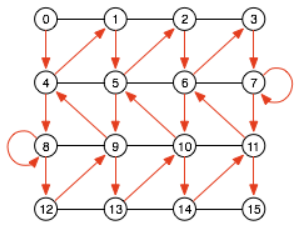
\includegraphics[width=0.6\textwidth]{figures/TriangleStripOrdering.PNG}
    \caption{Ordering of vertices in a triangle strip for a grid. Courtesy of \cite{triangleStrip}.}
    \label{fig:TriangleStrip}
\end{figure}

In this example, we can observe that on our path, we alternatively add 4 and subtract 3 for computing the next index, on the first row. On the next row, we still add 4, but subtract 5. The number 4 represents the number of vertices in the row or column, depending on how we advance($n + 1$ vertices, where n = number of divisions).
The numbers 3 and 5, correspond to $m = (n+1) + 1$ or $m = (n+1) - 1$ and represent changes between adjacent columns. The number alternates, depending on the order of traversal on that particular row.

This approach provides a decent reconstruction, for a 2.5D object using data from a single depth camera. Normals can also be computed after we have the geometry(at an additional computational cost), however, there is no need for lighting in our 3D scene, since we will be applying textures(which represent the desired image contents) on the mesh before rendering. For improving the visual quality of the mesh, one could also look at more sophisticated methods of triangulation such as \textit{Delaunay Triangulation}, or use standard 3D reconstruction techniques, like the \textit{Marching Cubes} algorithm.

\subsubsection{Other Methods for Triangulation}

Other methods of triangulating the mesh into either 2.5D or 3D objects will be shortly described in the next sections. An implementation of most of these methods has been attempted. However, the technique described in section \ref{sec:TriangleStripTriangulation} is the one which is currently used. Some of these alternatives were running either too slow, or were taking too long to implement.

\paragraph{Delaunay Triangulation}\mbox{}\\

The naive triangulation, by connecting the triangles without considering some measure of how natural it looks, may not provide the intuitively \textit{best-looking} results. If the triangulation is not acceptable, it can be improved with a technique such as \textbf{Delaunay Triangulation}(explained in detail in \cite[Chapter~9]{berg08}), where triangulations are ranked by comparing their smallest angle(small angles, result in \textit{skinniness}). This tecnhique can be used for 2.5D reconstruction and can obtain an optimal triangulation. For more information please consult appendix \ref{appendix:B-delaunay}.

\paragraph{Marching Cubes}\mbox{}\\

One of the classic computer algorithms for surface reconstruction is the \textit{Marching Cubes}  algorithm. An attempt was made to implement this algorithm. In order to run it on a GPU, one can use a \textit{geometry shader} or\textit{ histogram pyramids} with a regular vertex and fragment shader. The attempt consisted of porting an existing implementation of the geometry shader for fixed-pipeline OpenGL to modern OpenGL. Unfortunately, I did not get any geometry as output after running the algorithm, but there were also no errors. The problem is that I could not debug the shaders, since the tools I have tried did not work - some because of no support for modern OpenGL(3.0+) like \textit{glslDevil}, and others did not work on my laptop because it uses the \textit{nVidia Optimus} technology, as is the case for the \textit{nVidia nSight} debugging tool for \textit{Microsoft Visual Studio}. As this was taking too much time, I decided to go for a simpler approach, that should still prove appropriate for the real-time 3D reconstruction of the cloth, described in section \ref{sec:TriangleStripTriangulation}. Nevertheless I will briefly describe the algorithm in the following section. More information on how it can be implemented on a GPU is available in appendix \ref{appendix:B-mc}. This may be useful to look into, as an extension to the current project, if a higher quality mesh is desired(this method works well for 3D objects in general, and is not restricted to 2.5D, as is the case for the currently used method).

\paragraph{The Marching Cubes Algorithm}\mbox{}\\

It was originally designed to create triangle models  from 3D medical data - usually volumetric data, using voxels for representation(voxels are similar to pixels, only they exist in 3D space and can be represented as a cube). The algorithm also needs each vertex of the dataset to have a scalar value, that usually represents a property of the underlying data set. An example of such a voxel set is shown in figure \ref{fig:VoxelSet}. This value will be used to construct an isosurface, by comparing where vertices of the voxel edges intersect the surface(given a constant user-defined threshold or isovalue).

\begin{figure}[hbtp]
    \centering
    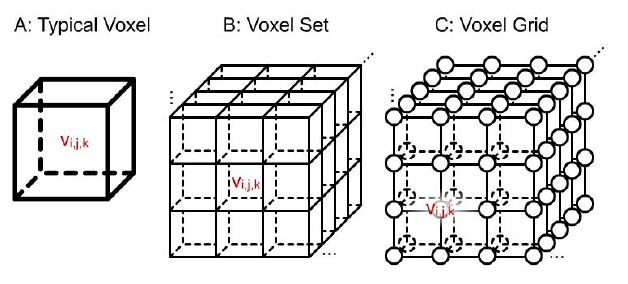
\includegraphics[width=0.4\textwidth]{figures/Voxels.PNG}
    \caption{Voxel data representation. Courtesy of \cite{navpreet2013}}
    \label{fig:VoxelSet}
\end{figure}


 The authors of the original paper on the topic state in \cite{william87} that two primary steps were used in their approach:
\begin{itemize}
\item Locating the surface corresponding to a user-specified value(isolevel) and creating triangles.
\item Calculating normals to the surface at each vertex of each triangle, in order to ensure a high quality image.
\end{itemize}

Since only the 3D mesh coordinates are required in order to capture the distortion of the cloth, the issue of calculating normals will not be described further, and we shall focus on the first part of the algorithm(although it should be mentioned that a fully shaded, reconstructed model could be useful for some calibration approaches, since, at the time of this writing there are no reconstruction libraries for the depth camera used in this project).

The algorithm uses a divide-and-conquer approach by using logical cubes of eight pixels to locate the surface. How the surface intersects every such cube needs to be determined. In order to do this, a value of one is assigned to a cube's vertex, if the data value at that vertex exceeds the value of the surface we are constructing(if the scalar value is above a threshold called the isolevel). These vertices are inside the surface. Conversely, a zero value is assigned to values below, and thus outside, the surface. The surface intersects the cube edges where one vertex is inside and the other outside.

Moreover, there are eight vertices in each cube and two states(inside and outside) so we have a total of $2^{8} = 256$ cases for intersection with such a cube. However, by eliminating symmetries, like complementary cases and rotational symmetry, the number of distinct cases of triangulation can be reduced to 14 patterns.

\begin{figure}[hbtp]
    \centering
    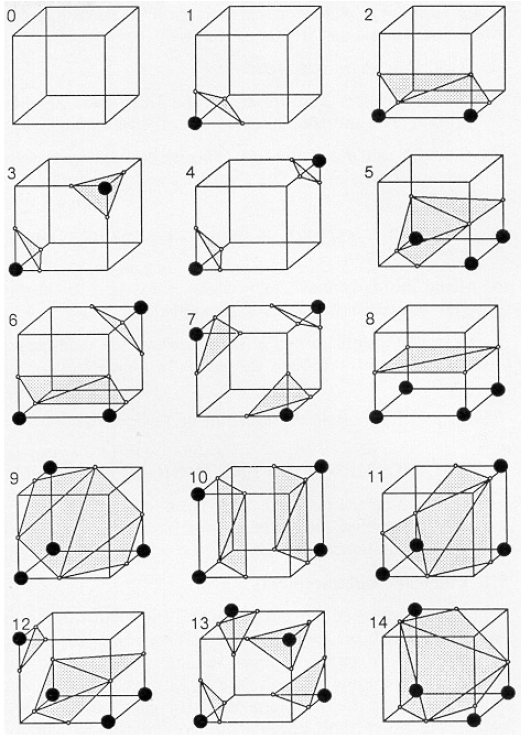
\includegraphics[width=0.4\textwidth]{figures/MarchingCubesTriagulationCases.PNG}
    \caption{Marching Cubes - The 14 Patterns of Triangulated Cubes. Courtesy of \cite{william87}}
    \label{fig:MarchingCubesTrianglatedCubes}
\end{figure}

As an example, the cube for pattern one in figure \ref{fig:MarchingCubesTrianglatedCubes} contains one  of the surface vertices(the lower-left vertex of the front face) and results in one triangle defined by three edge intersections. An eight bit index is created for each case, and it corresponds to the cube's vertex states(see figure \ref{fig:MarchingCubesLabeling}). This index points to an edge tables that retrieves all of the edge intersections for the given cube configuration. The triangles are calculated using linear interpolation of the scalar values along the vertices of the respective edges(to determine the exact location of the triangle vertices on the cube edges). As described in \cite{navpreet2013}, if $P1$ and $P2$ are the vertices of an intersected edge and $V1$ and $V2$ are the scalar values of each vertex, the intersection point $P$ is calculated as following:  
	$$P = P_{1} + (isovalue - V_{1})(P_{2} - P_{1}) / (V_{2} - V_{1})$$

\begin{figure}[hbtp]
    \centering
    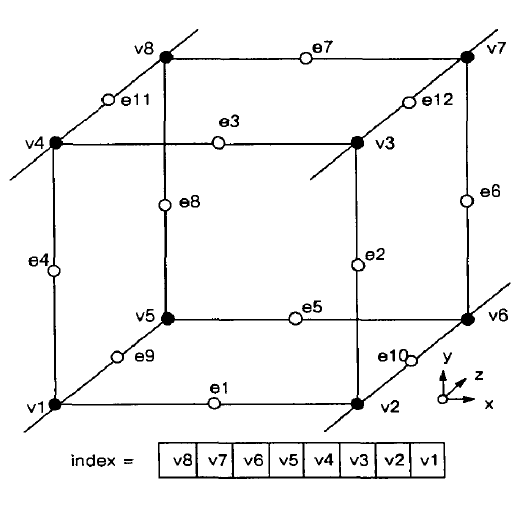
\includegraphics[width=0.4\textwidth]{figures/MarchingCubesNumbering.PNG}
    \caption{Marching Cubes - Cube Numbering. Courtesy of \cite{william87}}
    \label{fig:MarchingCubesLabeling}
\end{figure}



\paragraph{Greedy Triangulation}\mbox{}\\

Another triangulation method that was briefly considered was the greedy projection algorithm described in \cite{Marton09ICRA}. As described in the previously mentioned source as well as in \cite{navpreet2013}, the algorithm grows the mesh from a list of points, until all points have been considered or there are no more valid triangles to be formed - in case of the latter, the algorithm is restarted somewhere in the unconnected area with vertices from a new \textit{seed} triangle.

An implementation is available in the PCL library, and a description on how to use it can be found in \cite{PCLGreedy}. The algorithm has been tested on the bunny mesh that is mentioned in the PCL tutorial. The result was a triangulated mesh of the provided point cloud. The algorithm also computes the normals and a shaded model of the object is shown in figure \ref{fig:ReconstructedBunny}. However, this was a static object and it was only comprised of about 400 vertices. When the test was run on the point cloud retrieved by the depth camera, the algorithm was running very slow, and it was clear it could not achieve an interactive framerate - it was taking seconds or even minutes per frame, before giving warnings/errors about the dataset; the size of the point cloud was of about 70000 vertices. Indeed, in \cite{Marton09ICRA} it is mentioned that the algorithm is (only) near real-time. Further, a performance analysis is provided, where a point cloud of comparable size was reconstructed in about 9 seconds. Some of the parameters of the algorithm could perhaps be changed in order to improve performance(and remove the warnings), although, it is unlikely that this method will reach an interactive frame rate of about 30 frames per second or more. This is an important aspect to consider, as the distortion of the cloth display needs to update reasonably fast(at interactive speeds) in order for the system to be usable. Due to the previous reason and time constraints, the alternative described in section  \ref{sec:TriangleStripTriangulation} was employed.

For more information about the algorithm itself please consult appendix \ref{appendix:greedy}.

 
\begin{figure}[hbtp]
    \centering
    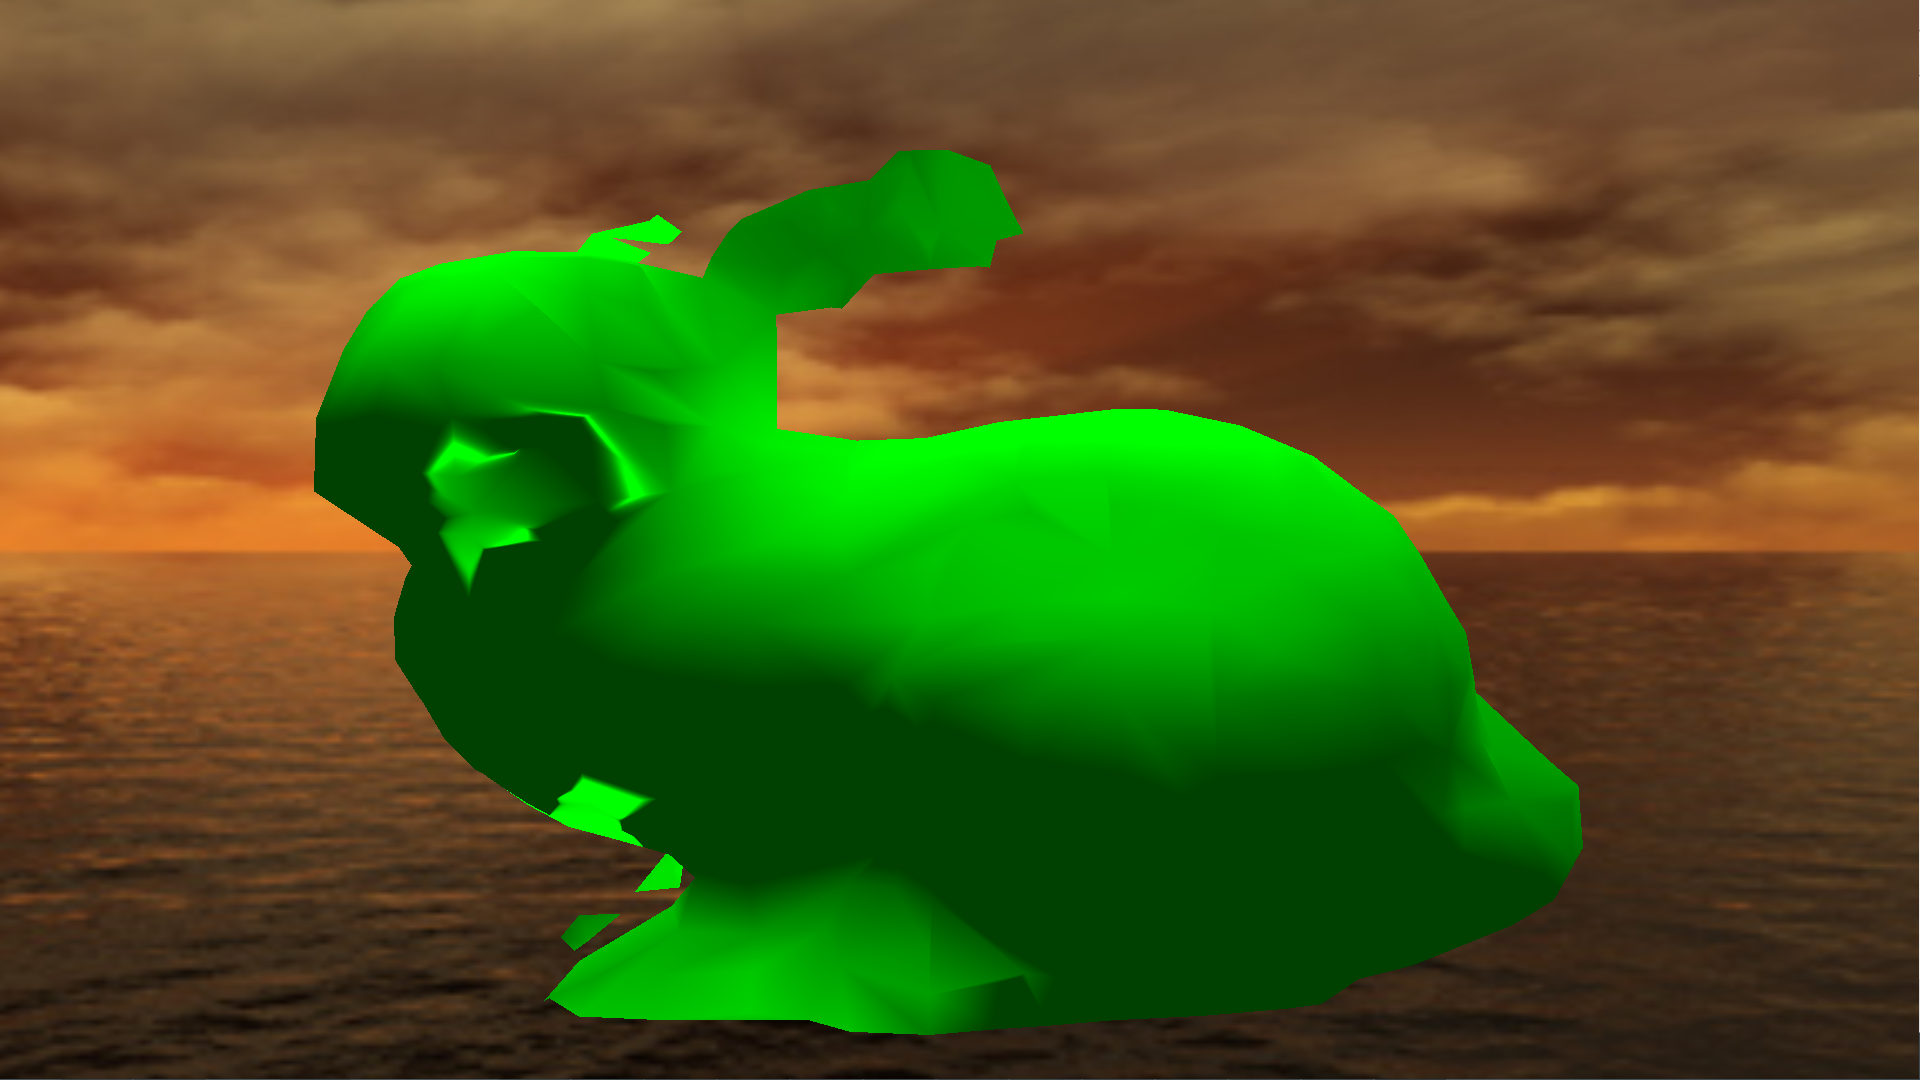
\includegraphics[width=0.4\textwidth]{figures/reconstructedBunny.png}
    \caption{Mesh from point cloud reconstruction of a bunny.}
    \label{fig:ReconstructedBunny}
\end{figure}

\subsection{Projective Texture Mapping}
\label{sec:ptm}

A white paper by \textit{NVIDIA} describes projective texture mapping and how it can be implemented using OpenGL (see \cite{cassNvidia}). They mention that the theoretical foundation for the method is described in \cite{segal92}. The white paper contains more useful information for implementation however; a short summary of this is presented below.

For projective texture mapping, we need to use homogeneous texture coordinates. For example, for a projective 2D texture we have the coordinates (s,t,q) where the interpolated homogeneous coordinate is projected to a real 2D texture coordinate by dividing both s and t by q to obtain, (s/q, t/q). The homogeneous texture coordinates have to be assigned per-vertex. The final step implies a range mapping with [0,1] for each coordinate (using a scale and bias, so that the texture coordinates change from [-1,1] to [0,1]). In figure \ref{fig:VirtualProjectorPipeline} the transforms that are applied to a vertex position in order to compute projective texture coordinates are displayed.

\begin{figure}[hbtp]
    \centering
    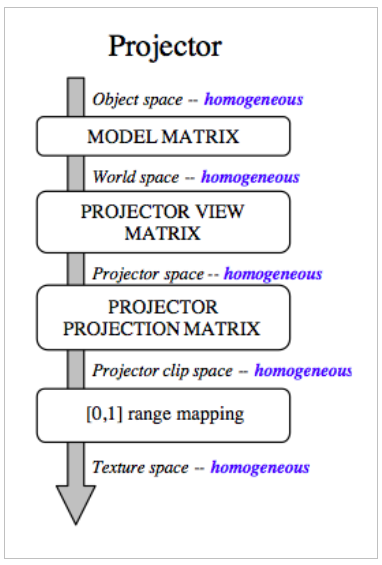
\includegraphics[width=0.4\textwidth]{figures/VirtualProjectorPipeline.PNG}
    \caption{Virtual Projector Transformation Pipeline. Courtesy of \cite{cassNvidia}}
    \label{fig:VirtualProjectorPipeline}
\end{figure}

The vertex position in object and eye space is used to generate the texture coordinate. In OpenGL this can be accomplished with the \textit{texgen} facility (generates texture coordinates from vector attributes). In the \textit{object} and \textit{eye linear} modes, the texture coordinate is computed by solving a plane equation at the vertex position. Evaluating a plane equation is equivalent to a 4-component dot product, so the texgen planes form a 4x4 matrix, $T$, as shown in figure \ref{fig:ProjectiveTextureMapping}.

\begin{figure}[hbtp]
    \centering
    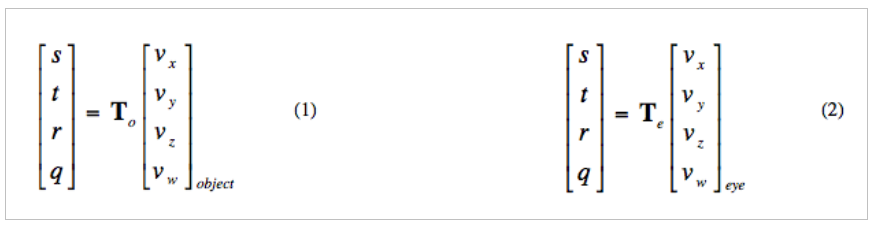
\includegraphics[width=1.0\textwidth]{figures/PTMCoordinates.PNG}
    \caption{Projective Texture Coordinates from a 4x4 matrix and the vertices in object or eye space, where $s, t, r, q$ are the texture coordinates, $v$ represents the vertices in \textit{eye} or \textit{object} space and $T$ is the texgen matrix in eye or object space. Courtesy of \cite{cassNvidia}}
    \label{fig:ProjectiveTextureMapping}
\end{figure}

\subsubsection{Object Linear Texgen}

The object linear texgen can be represented as shown in figure \ref{fig:ObjectLinearTexgen}, where the first matrix is the scale-bias matrix, $M$ is the model matrix, $V_{p}$ is the view matrix for the projector and $P_{p}$ is the projector's projection matrix.

\begin{figure}[hbtp]
    \centering
    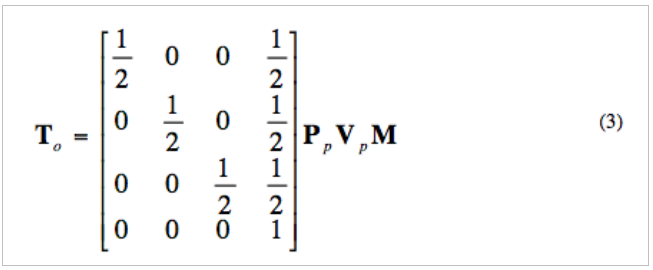
\includegraphics[width=0.6\textwidth]{figures/ObjectLinearTexgen.PNG}
    \caption{Object Linear Texgen. Courtesy of \cite{cassNvidia}}
    \label{fig:ObjectLinearTexgen}
\end{figure}

\subsubsection{Eye Linear Texgen}

The eye linear texgen can be represented as shown in figure \ref{fig:EyeLinearTexgen}, where the same notations are used as in the previous section, but instead of multiplying with the model matrix $M$ in the end, we multiply with $V^{-1}_{e}$ which is the inverse of the eye(or camera) view matrix.

\begin{figure}[hbtp]
    \centering
    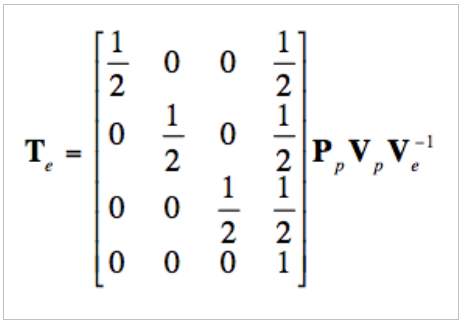
\includegraphics[width=0.4\textwidth]{figures/EyeLinearTexgen.PNG}
    \caption{Eye Linear Texgen. Courtesy of \cite{cassNvidia}}
    \label{fig:EyeLinearTexgen}
\end{figure}

\subsection{Capturing Dynamic Contents}

Dynamic contents can be obtained by simply rendering textures every frame. Currently, they must be stored and initialized before the application is started. However, in order to create a versatile system, it is required to capture the contents of another application and then pass them to the distortion correction application for rendering - this could be implemented as future work. The window capturing is operating system specific. Finally, an interaction API of the display would have to communicate with the underlying application, sending commands as appropriate.

\newpage
\section{System Development and Implementation}

In this chapter I will go into detail about how the employed methods  were implemented, as well as presenting the results of a particular step, including tests, if required. Further more, the explanations will be backed with main coding samples. This chapter will include information on the tools and frameworks used, 3D engine setup, creation of the point cloud, mesh rendering and triangulation, projective texture mapping, noise reducing methods and manual alignment of physical and virtual cameras and components.

\subsection{Tools and Technologies Used}

The prototype has been implemented in C++ using \textit{OpenGL v3.3}, which uses the programmable OpenGL pipeline(the vertex and fragment shaders must be programmed to suit the problem's specific needs). This means that shaders must be used to render graphics on the screen. This choice was made because of performance improvements over the OpenGL immediate mode, as well as allowing the code to take advantage of the latest OpenGL features, in possible future extensions.

The development environment used was the \textit{Microsoft Visual Studio IDE}. Initially, development started on the 2013 version of the IDE, but due to incompatibilities with some of libraries used, the toolchain was switched to that of \textit{Visual Studio 2012}(while still using the 2013 IDE - in order to do this, both versions need to be installed). Note that the professional edition of \textit{Visual Studio} is needed in order to be able to install the plug-in for syntax highlighting of shader files.

Further, several libraries were used to create a simple graphics engine that can be used to render objects, import meshes, move around a virtual world etc. The \textit{GLEW}(see \cite{glew}) library was used for importing the OpenGL functions and extensions into the project, while the \textit{GLFW}(available at \cite{glfw}) library was used for managing the window context, as well as for managing keyboard and mouse input.

Another useful feature is to be able to import textures and apply them to objects in the 3D world. The \textit{FreeImage} library(available at \cite{freeimage}) has been used for reading in images and checking if the format is correct. Further, objects can be imported from standard graphics programs through ASSIMP(details at \cite{assimp}), using well-known file formats like \textit{WaveFront OBJ} and \textit{Autodesk 3DS}. This feature was useful when debugging different aspects of the graphics engine and it was also used to test projective texture mapping on a physical ball, by using an imported mesh of the interior half of a sphere.

Another important library is \textit{GLM}(available at \cite{GLM}), which contains very useful math functions, like the ability to work with matrices and vectors, calculating the inverse of a matrix etc. In addition, this library uses the same syntax as that of GLSL(OpenGL Shading Language), which means that there is more consistency in the code and there is no need to learn a third-party syntax.

Further, the \textit{Point Cloud Library}(PCL, available at \cite{PCL}) was used for trying out some reconstructions techniques, like the greedy projection triangulation. However, this library has not been used in the final implementation, as the mesh was triangulated by connecting a triangle strip, using the fact that the point cloud was ordered, to connect adjacent points.

Finally, the only other library used was the \textit{Intel Perceptual Computing SDK}(details at \cite{PCSDK}) which can be used to retrieve the depth and color streams, and to do some basic image processing. For this project, only the depth stream was used. The data was quite noisy, so in order to reduce noise, some depth smoothing functions were applied. These will be described in one of the future sections. Otherwise, the library allows one to easily convert the data from the depth camera to a point cloud, as well as to unproject it to 3D space, as described in the following sections.

\subsection{Virtual World Setup}


The process to set up the virtual world will not be described in detail here. The structure of the code was inspired by the OpenGL tutorials available at \cite{OpenGLTuts}, as well as several other on-line articles/tutorials describing OpenGL functionality. Basic functionality is contained in a class, or cpp file - for example, all texture related processing is the responsibility of the \textit{Texture} class, shader programs are compiled and linked by the \textit{LoadShader} method defined in \textit{loadShader}.h/.cpp, etc. Next, the 3D world is created as a scene(indeed, several such scenes were creating during development, for testing purposes). Each scene must implement three different methods, inheriting from a \textit{SimpleScene} class:
\begin{itemize}
\item $initScene(GLFWwindow *window)$ - used to initialize everything that is needed before rendering, for example, the compilation and linking of shader programs is done at this stage
\item $renderScene(GLFWwindow *window)$ - this method loops continuously; it is called every frame, and it is responsible for the actual rendering that can be observed on the screen
\item $releaseScene()$ - this is mainly used for memory deallocation and is called before the application exits
\end{itemize}

This template can be used to create new scenes, and all basic functionality such as texture and object importing, camera movement, shader compilation and linking, shaded/unshaded rendering by using different vertex and fragment shader programs, are already available and can be easily reused.

% %\subsection{Rendering}
\subsection{Point Cloud Generation}

The \textit{RawDepthPipeline} class is responsible for retrieving video frames from the depth stream. A method has been added, $renderFrame(..)$ that simply acquires the current frame so that the data can be converted to a point cloud, and subsequently a mesh. If the frame data is valid, a call is made to $createPointCloudMappedToWorld$ which is the function responsible for converting the raw data into a 3D point cloud, in world coordinates.

An array is needed to store the point cloud:


\begin{verbatim}pcPos = (PXCPoint3DF32*)new PXCPoint3DF32[nPoints].\end{verbatim} 


The data type is from the Intel Perceptual Computing library and represents 3D points with $x,y,z$ coordinates and floating point values. Further, the number of points, namely \verb|nPoints|, is set tot the maximum number of elements we could have in the cloud, which is equal to \verb|depthCamWidth*depthCamHeight|, where the previous two variables represent the width and height of the depth frame, respectively. Then, we just need to iterate over all the depth values and retrieve the depth value:

 \begin{verbatim}pxcU16 depthValue = 
     ((pxcU16*)ddepth.planes[0])[y * depthStride + x],\end{verbatim} 
 
 
where \verb|ddepth.planes[0]| is an array containing the depth data, and  \verb|x| and \verb|y| represent the current index on the height, and width of the image, respectively. The \verb|depthStride| is used to properly access a two-dimensional array using one index, and it represents the width of the row. Finally, we check if the depth value is in a certain range, and, if so, it is stored in our \verb|pcPos| array:
\begin{verbatim}
if (depthValue > 10 && depthValue < 2000)
	{
		pcPos[n].x = (pxcF32)x;
		pcPos[n].y = (pxcF32)y;
		pcPos[n].z = (pxcF32)depthValue;	
	}
n++;
\end{verbatim}
The elements in the array for which we do not have valid depth values remain uninitialized($n$ is incremented irrespective of the depth value). This is required, because when we send the array later to an \textit{OpenGL VBO(Vertex Buffer Object)}, all valid elements are rendered. This means that initializing the values with, for example \verb|(0, 0 ,0)|, would result in a lot of points connected to the origin point \verb|(0, 0 ,0)|, which is not desired.

The last thing that needs to be done at this stage is to unproject the points to 3D space. In order to do this, one needs to know the depth camera's intrinsic calibration parameters(these parameters relate to the field of view of the camera, distortion coefficients, principal point etc.). However, the Intel Perceptual Computing SDK provides a very handy method that does the necessary computation for us:

\begin{verbatim}projection->ProjectImageToRealWorld(nPoints, 
    &pcPos[0], worldPos.data()).\end{verbatim}

The $worldPos$ vector array will contain the final points that will be rendered on screen. If we were to render the image now, we would get a 3D point cloud representation of our depth stream. Therefore, the final issue which remains is to connect the points in order to form a mesh, so that the texture will be projected on a polygonal surface. This process will be described in he following section. 

\subsection{Mesh Rendering}

\subsubsection{Rendering Process}

In order to render a mesh that changes every frame at an acceptable speed, the use of OpenGL VBOs has been employed. This object is nothing more than a contiguous untyped block of memory(untyped means it does not have a particular structure; the structure is defined by the user as we shall see shortly), which can be used to store several vertex arrays and upload them to the GPU. A vertex array is usually used to store a specific vertex property, such as position, color etc. For an example of an interleaved vertex array with two attributes(position and color), please consult figure \ref{fig:VertexArrays}. Note that we are only interested in position for our mesh, since we will only use one full color of the mesh for debugging purposes and, the user will only see the color of the texture.

\begin{figure}[hbtp]
    \centering
    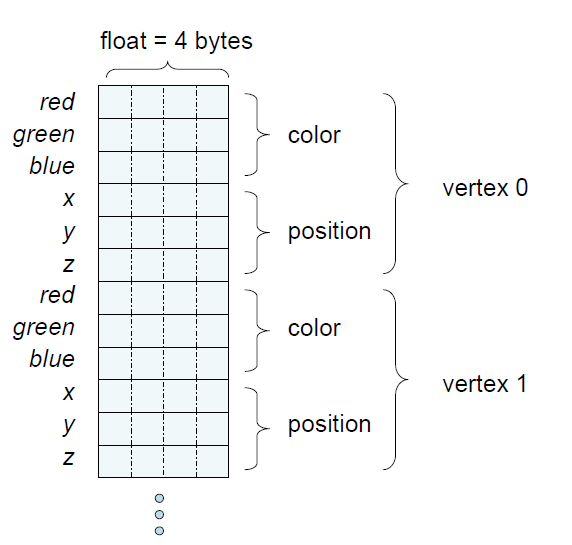
\includegraphics[width=0.7\textwidth]{figures/VertexArrays.PNG}
    \caption{Vertex array layout with two vertex attributes. Courtesy of \cite{kilgard2009}}
    \label{fig:VertexArrays}
\end{figure}

A good resource that explains how to properly use VBOs in OpenGL and why they are needed is \cite{kilgard2009}. The author explains that the GPU doesn't have arbitrary access to conventional system memory(so called client memory). With VBOs one can point the GPU at the vertex arrays and let it read the vertex attributes from the arrays contained inside it(the arrays are stored in spatially negotiated regions of memory, maintained as buffer objects, that both the application and the OpenGL implementation can access). An example of how the VBO data is transferred to the GPU via DMA(direct memory access) transfers is shown in figure \ref{fig:VBOClientMemory}. As you can see from the figure, there is no communication between the data and the CPU, all transfers are made using DMA transfers directly to the GPU. This means that the performance can be greatly improved by avoiding unnecessary communication with the CPU. This is in stark contrast with the OpenGL immediate mode, where each call to \verb|glBegin()| and \verb|glEnd()| had to be sent first to the CPU, in addition to a full list of commands for drawing(now we just draw the VBO with one call to \verb|glDrawArrays| or \verb|glDrawElements|).
\begin{figure}[hbtp]
    \centering
    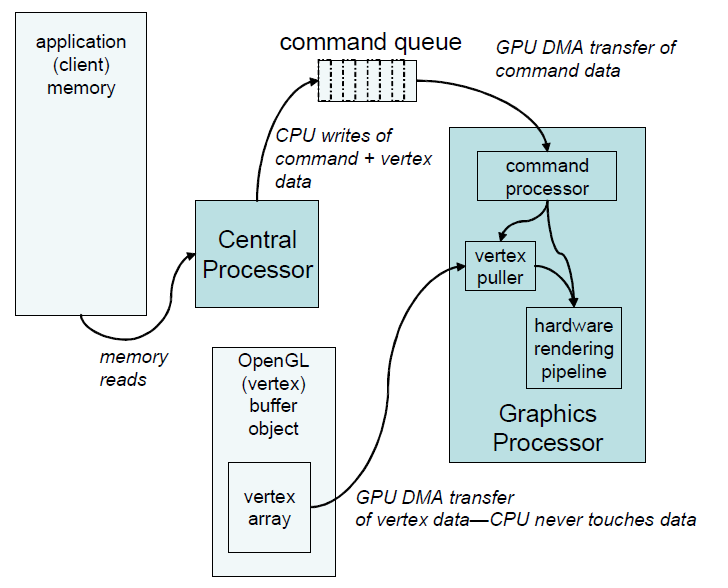
\includegraphics[width=0.85\textwidth]{figures/VBOClientMemory.PNG}
    \caption{Transfers of vertex array object data using DMA.}
    \label{fig:VBOClientMemory}
\end{figure}

We need to define the type of data and how much of it needs to be stored in a VBO. In order to do this we use a vertex attribute pointer:
\begin{verbatim}
// vertex positions start at index 0
// the distance between two consecutive vertices is
// sizeof whole vertex data
glEnableVertexAttribArray(0);
glVertexAttribPointer(0, 3, GL_FLOAT, GL_FALSE, 
    sizeof(PXCPoint3DF32), 0);
\end{verbatim}
The signature of the vertex attribute pointer method is as follows:

\begin{verbatim}
void glVertexAttribPointer(GLuint index​, GLint size​, GLenum type,
 GLboolean normalized​, GLsizei stride​, const GLvoid * pointer​)
\end{verbatim}

In the previous code we enable the vertex array with index 0. The \textit{glVertexAttribPointer} is also set to  index 0(first parameter), since it is the one and only attribute(for example, we could interleave data, if we also had texture coordinates; then the index would be 1 since 0 would have already been used by the position attribute). In it we can store data with 3 components: $x,y,z$ and we specify the size of $PXCPoint3DF32$. The size will be used as an offset to store the next vertex(stride). We only store the point cloud elements in this VBO and, therefore, we can just set the pointer to 0, as there is no other data stored in the VBO.

Before a VBO has to be used, it must be bound, so that it is made the active VBO. The custom class \textit{VertexBufferObject} provides methods so that we can easily create and bind VBOs, like so:
\begin{verbatim}
// create and bind VBO
vboSceneObjects.createVBO();
vboSceneObjects.bindVBO();
\end{verbatim}

Now that our VBO is bound, we need to add the actual data:

\begin{verbatim}
glBufferData(GL_ARRAY_BUFFER, rdp->nPoints * sizeof(PXCPoint3DF32), 
NULL, GL_STREAM_DRAW);
\end{verbatim}

This line stores an array buffer of n points of the Intel Perceptual Computing point type. Further, the hint \verb|GL_STREAM_DRAW| indicates that our data will be constantly updating(every frame). This makes OpenGL optimize the VBO for dynamic contents. Another flag, \verb|GL_DYNAMIC_DRAW| is available, but this is actually for dynamic data that does not change every frame, only at specific moments. So, in this case, the first flag is the appropriate one, since the mesh will be updated every frame.

OpenGL also has another data type, namely the VAO(Vertex Array Object) which can store multiple VBOs. These VAOs are mainly used to avoid setting the vertex attribute pointers each time we bind the VBO. We just bind the VAO, and we do not have to do anything else. Now, if we were to render our memory contents using $glDrawArrays$, we would need to draw the type \verb|GL_POINTS|. This is because we have not triangulated the point cloud yet.

\subsubsection{Triangulation}

As described in section \ref{sec:TriangleStripTriangulation} a triangle strip has been used to triangulate the point cloud. In order to do so, an \textit{IBO(Index Buffer Object)} has been used to store a \verb|GL_ELEMENT_ARRAY_BUFFER|. This object is very similar to a VBO, the only difference is that we do not store vertex attributes in the element array, but actual element indices. In other words, we need to compute an array of indices, that defines how the triangle strip should be connected, and then just simply bind the data to the IBO:
\begin{verbatim}
ibo.addData(&(rdp->indices[0]), 
    rdp->indices.size() * sizeof(unsigned int));
ibo.uploadDataToGPU(GL_STATIC_DRAW);
\end{verbatim}

We add an array of \verb|int|s into the buffer object of the size of the depth camera's resolution, in pixels(\verb|width*height|). Note that the index computation can only be done once! We always have the same indices, for the same grid, since the x and y values are fixed for a vertex - the indices are computed for all points, even for invalid ones, this means we do not have to recompute the indices if the state of the points changes(since the VBO data for those invalid points is not initialized, they will not be drawn). This means the flag for data optimization has been set to \verb|GL_STATIC_DRAW|. Further, the \verb|uploadDataToGPU| method internally calls  \verb|glBufferData| with the previously added element array data. Finally, the IBO is bound and setup similarly to a VBO.

The drawing command in order to render a mesh from the indices(connected using a triangle strip), is:
\begin{verbatim}
glDrawElements(
	GL_TRIANGLE_STRIP,      // mode
	rdp->indices.size(),    // count
	GL_UNSIGNED_INT,   // type
	(void*)0           // element array buffer offset
	);
\end{verbatim}

The parameters are briefly explained in the comments, but to detail briefly:
\begin{itemize}
\item the first parameter is the type of primitive OpenGL will use for rendering
\item the second parameter represents the number of elements required to draw the mesh
\item the third parameter defines the type of the elements 
\item finally, the last parameter is simply a pointer that defines an offset, but since we only have the mesh data to render with indices, this can be set to 0
\end{itemize}
 
 The only thing left to be is explained is how the index array has been populated. In order to understand how the code works, it is useful to review figure \ref{fig:TriangleStrip}. The logic is contained in the \verb|addIndexData| method from the \textit{RawDepthPipeline} class. We traverse the two-dimesional grid with one index(in the same manner as we have traversed the depth frame before):

 \begin{verbatim}t = c + r * colSteps,\end{verbatim}
 
 where \verb|t| will represent our current position in the grid. As we can see from the previously mentioned figure, the indices are connected by using elements from adjacent rows, alternatively.We can then simply check if this position is divisble by 2 or not, so we know if we need to move to the other row. We first push index 0, and then we need to add the width of the grid to our current index(since it is divisble by 2):
 \begin{verbatim}
if (t % 2 == 0) {
	n += width;
}
 \end{verbatim}
In the next iteration, we go in the \verb|else| loop and check if the index of the row is divisible by 2. This is required, since we traverse the grid from both directions and we need to subtract \verb|width-1| or \verb|width+1|, in order to traverse up with one row, depending on whether we are traversing the current row from left to right, or right to left, respectively:
\begin{verbatim}
(r % 2 == 0) ? n -= (width - 1) : n -= (width + 1);
\end{verbatim}
Then, the process is simply repeated. Note that, since we pass through two rows in one direction, \verb|colSteps| is set to \verb|width * 2|(for example, the last element in the second row in the figure is $7$, which is element number 4*2 = 8, since our width is 4 in that example). Further, we stop one row before the last, since we traverse through the last one, when we start on the one right before it, so \verb|rowSteps = height - 1|.

Finally, we need to remember to add the degenerate triangle by adding the last index twice(once as shown below, and again at the start of the next loop, as \verb|r| is incremented):
\begin{verbatim}
if (c == colSteps - 1) {
	indices.push_back(n);
}
\end{verbatim}

At the end of this process, the \verb|indices| vector will contain all of the triangle strip indices and in the right order. Therefore, it can be added to the index buffer object, so that the data is available for rendering later(degenerate triangles will simply be discarded by the GPU, they will not introduce artifacts).

\subsection{Depth Smoothing}
\label{sec:DepthSmoothing}
The depth data is quite noisy and, due to this, the final textured image is shimmering(vertices are moving around between frames, which creates a distracting effect). The effect is similar to aliasing(the "staircase effect").

In order to reduce this noise, smoothing of the depth data can be applied. A whitepaper from Canesta(see \cite{gokturk}) discusses aliasing issues, as well as artefacts for time-of-flight cameras. The authors describe how the noise can be reduced through \textit{spatial} and \textit{temporal averaging}. 

Further, they suggest the use of a median filter for improving resolution, as a solution for spatial averaging. They applied a $5 \times 5$ median filter and noticed a two-fold increase in resolution. 

Next, they present a case where 10 frames were averaged over time. Their results indicate that this technique of temporal averaging made the image much clearer and considerably increased the resolution.

In the following sections the implementations for spatial and temporal averaging employed in this project will be described.

\subsubsection{Spatial Averaging}

A median filter is used as a means for spatial averaging. The basic idea is to form a window of size $N \times N$, where $N$ is an odd number(greater than 1, otherwise we would have just one element in the window). Typical values for $N$ are $3$, $5$ or $7$. We traverse with such a window through the whole image, with the current pixel(or vertex) being in the center of the window, and the other elements being the immediate neighbors. Further, we need to obtain the \verb|median| of the window. The median is the center element of a sorted array. Therefore, we also need to apply a sorting algorithm. Insertion sort is typically used for median filter implementations, since it is efficient for small data sets.

The median filter can bet turned off and on by the press of a key, using a boolean variable. The size of the window must be specified before, since it is represented as a constant. The \textit{medianFilter} method in the \textit{RawDepthPipeline} computes the result for every frame, based on the specified \verb|windowSize|. In order to do this, the fact that both index digits of the center element in the window are: \verb|midIndex = (size - 1) / 2| is used(here \verb|size| is equal to the \verb|N| mentioned above). To compute the window elements, we traverse it using \verb|for| loops and then assign the values like so:
\begin{verbatim}
window[index] = pcPos[(y - midIndex + i) * depthCamWidth 
			  + (x - midIndex + j)].z;
index++;
\end{verbatim}

We simply need to subtract \verb|midIndex| from the current position, in order to get the neighbor elements. For example, \verb|midIndex| would be equal to $1$, for a $3 \times 3$ window. Then \verb|window[0] = pcPos[(y-1)* depthCamWidth  + (x-1)]|, ..., \verb|window[8] = pcPos[(y+1)* depthCamWidth  +(x+1)]| .

Once we have the elements, we need to sort them, in order to find the median. Insertion sort was used to accomplish this: \verb|insertionSort(window)|. Now we simply need to assign the median as the new depth value for the current point, and continue to iterate through the rest of the points.

Additionally, we must only apply the algorithm if all the neighbors of the current point have valid depth values(since certain areas of the image do not contain depth information), so this must also be checked.

The sorting method works by iterating through each element of the array, storing it(\verb|temp = window[i]|) and then comparing it against the size of all elements to the left of \verb|temp|. The left side represents the sorted part of the array(we start with the left-most element). If the current element is less than another one from the left of the list, the larger element is shifted one place to the right.
\begin{verbatim}
for (j = i - 1; j >= 0 && temp < window[j]; j--){
		window[j + 1] = window[j];
}
window[j + 1] = temp;
\end{verbatim}

The last line places the current element in its proper place. If it is the largest element in the left side of the list, \verb|j| will not be decremented and it remains on its current position. Otherwise, it is moved to the left, depending on how many elements are less than the current value. 		


\subsubsection{Temporal Averaging}

A WMA(Weighted Moving Average) algorithm has been used for temporal averaging. The main purpose of this is to average the depth information over the last $N$ frames. We assign weights or priorities to the frames, with the last frame having the highest priority when averaging.

The frame data is stored in a list from which we can push and pop elements(individual frame data arrays):
\begin{verbatim}
// push array to the back of the list
averageList.push_back(pcPos);
\end{verbatim}

Once we push a new frame in the list, we also need to check if the size of the list is greater than the number of frames we need to average over(we call \textit{checkForDequeue}). If so, we remove the extra frames from the list.
\begin{verbatim}
if (averageList.size() > averageFrameCount)
	{
		delete[] averageList.front();
		averageList.pop_front();
		checkForDequeue();
	}
\end{verbatim}

Next, we iterate through all of the arrays in the list, and compute the sum of the depth data for each element, with a weight that is 1 for the oldest frame, and $N$(currently 10) for the newest:
\begin{verbatim}
// count denotes the weight
sumDepthArray[index] += (pxcF32)item[index].z * count;
\end{verbatim}

Further, we also store a denominator we will use to compute the average: \verb|denominator += count|(we count how many times in total we add depth values from frames). Note that we need to finish this pass through all frames, in order to obtain all the sum values and the denominator.

Finally, we must iterate through the sum values and compute the average:
\begin{verbatim}
averagedDepthArray[index].z = 
	(pxcF32)(sumDepthArray[index] / denominator);
\end{verbatim}

In order to speed up the process, we can use a \verb|parallel_for| loop, so that the rows are processed in parallel. This is possible because the calculations are independent.
\begin{verbatim}
// Process each row in parallel
Concurrency::parallel_for(0, depthCamHeight,
		[&](int depthArrayRowIndex)
{
	...
}
\end{verbatim}

\subsubsection{Results}

The averaging techniques have been tested on the deformable display, by judging the quality of a texture with a grid on it. This makes it easier to notice noise around the grid's lines. In figure \ref{fig:GridNoiseReduction}, the difference between the grid texture with no averaging applied, and with both averaging techniques applied, is shown(the image is zoomed in so that the differences are easier to spot).

\begin{figure}
\centering
\begin{subfigure}{.5\textwidth}
  \centering
  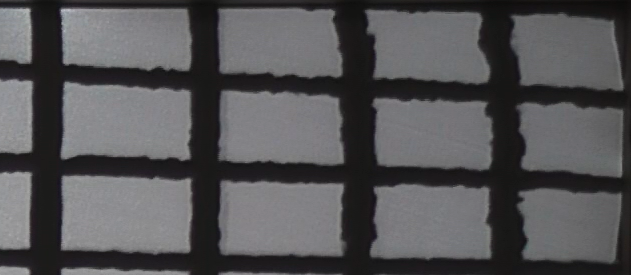
\includegraphics[width=0.9\linewidth]{figures/NoSmoothingC.png}
  \caption{Grid Before Averaging}
  \label{fig:GridNoAveraging}
\end{subfigure}%
\begin{subfigure}{.5\textwidth}
  \centering
  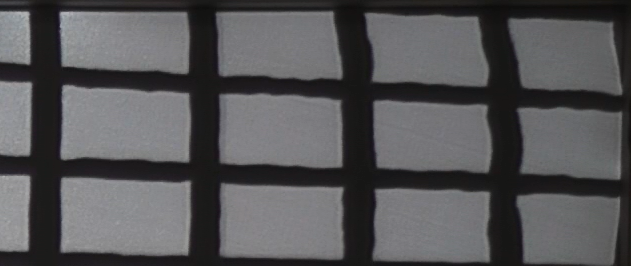
\includegraphics[width=0.9\linewidth]{figures/BothAveragingTechniquesC.png}
  \caption{Grid With Both Averaging Techniques}
  \label{fig:GridWithAveraging}
\end{subfigure}
\caption{A grid texture which shows the noise reduction obtained by averaging.}
\label{fig:GridNoiseReduction}
\end{figure}

Note that it is easier to see the differences in the thesis' video(see appendix \ref{appendix:A}), although it is still possible to see a significant difference in the figures. A downside of averaging is the reduction of frame rate. A $3 \times 3$ median filter was used in the final implementation, and a 10 frame moving weighted average was used as a temporal averaging technique. In table \ref{tabel:FrameRateReductionDueToAveraging} some data about the frame rate is presented, when turning on and off different averaging techniques. The frame rate was printed out for a certain number of frames, every second. The tests were also repeated 2-3 times and the results seemed consistent. We can see that the temporal averaging technique only slightly reduced the frame rate, while the median filter drastically reduced it, almost halving it when a 3x3 filter was applied, and almost halving it again, when a $5 \times 5$ filter was applied.

\begin{table}
\begin{center}
    \begin{tabular}{ | l | l |}
    \hline
    Averaging & Frame Rate \\ \hline
    None & ~[55 - 60] \\ \hline
    Temporal & ~[50 - 57] \\ \hline
    Both(3x3 MF) & ~[30 - 40] \\ \hline
    Both(5x5 MF) & ~[12 - 21] \\
    \hline
    \end{tabular}    
    
\end{center}
\caption{Frame Rate Comparison When Using Noise Reduction Techniques}
\label{tabel:FrameRateReductionDueToAveraging}
\end{table}

In order to improve the performance, the median filter could be applied on the GPU, by using shaders. One such method  is described in \cite{park}. They only briefly describe the method, but provide source code and a reference where the full algorithm is explain.

Finally, all averaging techniques can also reduce detail. For example, they could make the distortion correction less pronounced. This issue has not been thoroughly tested, and needs to be determined as future work. In order to properly analyze the previous issue, the calibration of the system should also be corrected, because then it would be easier to compare with the expected result.Moreover, one issue maybe that the distance and field of view of the virtual camera were set by trial and error. This is important because distance affects both the noise amount, as well as the degree to which the distortion correction can be seen.

\subsection{Projective Texture Mapping}

In order to get a final image rendered with the distortion compensation, by using a mesh of the deformable surface, one can apply projective texture mapping(\textbf{PTM}), as described in section \ref{sec:ptm}. This method was implemented using GLSL shaders.

However, before the implementation on the cloth display, the technique was tested in a virtual world(see figure \ref{fig:PTMTest}). Further more, to test if the technique is adequate for distortion correction, images were projected onto a ball using a physical projector, while applying a texture to the inside of a half-sphere in a 3D scene. This was used to counteract the distortion from the ball - the idea was to create the same effect as a pull gesture on a deformable display(in the 3D world, we would have a hole). The results are shown in figure \ref{fig:BallProjection} and although the images are blurry, it is possible to notice that lines are slightly more curved in the left image(for example, when looking at the second horizontal grid line from the top). The compensation amount varies depending on the properties of the virtual camera. Since the system was not calibrated, the results only slightly improved the aspect of the image. However, the important point is that a difference was observed and work then started to reconstruct the mesh of the cloth and project the texture onto it.


\begin{figure}
\centering
\begin{subfigure}{.5\textwidth}
  \centering
  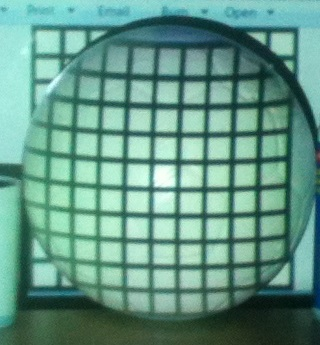
\includegraphics[width=0.9\linewidth, height=5cm]{figures/BallUncompensated.jpg}
  \caption{Image viewed normally.}
  \label{fig:BallNotCompensated}
\end{subfigure}%
\begin{subfigure}{.5\textwidth}
  \centering
  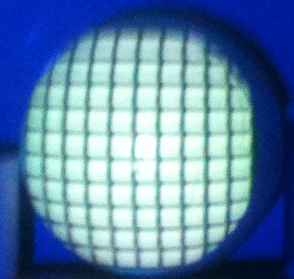
\includegraphics[width=0.9\linewidth, height=5cm]{figures/BallCompensated.png}
  \caption{Virtual projection shown.}
  \label{fig:BallCompensated}
\end{subfigure}
\caption{Comparison of projections on a physical ball.}
\label{fig:BallProjection}
\end{figure}

\subsubsection{Setting Uniforms and Computing the Texture Coordinates in the Vertex Shader}

Since the programmable OpenGL pipeline was used, there is no predefined \verb|Texgen| matrix. Instead, we can just use any $4 \times 4$ matrix. This matrix is defined as a uniform in the vertex shader(OpenGL server side code):
\begin{verbatim}
uniform mat4 TexGenMat;
uniform mat4 InvViewMat;
\end{verbatim}

The matrices are set from the OpenGL client code(the actual C++ application). The inverse view matrix is needed in order to convert from eye to world coordinates. In addition to these PTM specific matrices, we also need the usual projection and modelview matrix, as well as the position of the vertices:
\begin{verbatim}
uniform mat4 P;
uniform mat4 MV;
layout (location = 0) in vec3 inPosition;
\end{verbatim}

We need to compute the texture coordinates for the projected texture and pass them to the fragment shader:
\begin{verbatim}
out vec4 projCoords;
vec4 posEye    = MV * vec4(inPosition, 1.0);
vec4 posWorld  = InvViewMat * posEye;
projCoords     = TexGenMat * posWorld;
\end{verbatim}

The \verb|TexGenMat| has been constructed as described in section \ref{sec:ptm}, in the object linear texgen equation, except the final multiplication with \verb|M|:
\begin{verbatim}
texGenMatrix = biasMatrix * projectorP * projectorV;
invViewMatrix = glm::inverse(mModelView);
\end{verbatim} 

Actually, by the time we compute the inverse, in the second line of the code above, \verb|mModelView| only contains the view matrix. The modelview matrix uniform is instead stored from another variable, called \verb|mCurrent|:
\begin{verbatim}
glUniformMatrix4fv(iPTMModelViewLoc, 1, GL_FALSE, 
glm::value_ptr(mCurrent));
\end{verbatim}

The \verb|glUniformMatrix4fv| method binds the given matrix to the location of the modelview matrix in the shader. The 4 in the name, means OpenGL is expecting a $4 \times 4$ matrix, and the $v$ at the end denotes a vector or pointer array, which we will need to pass in as the data. The proper location can be retrieved from the shader program ID and a string which corresponds to the name of the variable:
\begin{verbatim}
int iPTMModelViewLoc = glGetUniformLocation(programID, "MV")
\end{verbatim}
The other uniforms are set in a similar way(if we just need to bind an integer we use \verb|glUniform1i|).We set the projection matrix, the texgen matrix, the inverse view matrix, and finally sampler locations, color locations and a debug uniform. The samplers, colors and debug uniforms are only used in the fragment shader, while the others are needed in the vertex shader. 
%\begin{verbatim}
%glUniformMatrix4fv(iPTMProjectionLoc, 1, GL_FALSE, 
%    glm::value_ptr(*pipeline->getProjectionMatrix()));
%glUniformMatrix4fv(iTexGenMatLoc, 1, GL_FALSE, 
%    glm::value_ptr(texGenMatrix));
%glUniformMatrix4fv(iInvViewMatrix, 1, GL_FALSE, 
%    glm::value_ptr(invViewMatrix));
%glUniform1i(iSamplerPTMLoc, 0);
%glUniform1i(iProjSamplerLoc, 1);
%//black
%glUniform4fv(iColorLoc, 1, glm::value_ptr(glm::vec4(0.0f, 0.0f, 0.0f, 1.0f)));
%// update debug state
%glUniform1i(iDebugLoc, bFragmentShaderDebug);
%\end{verbatim}

Finally, we need to apply the model matrix, in order to get world coordinates. First, the eye coordinates are computed(multiplying with the modelview matrix). Then, in order to get the world coordinates, we need to remove the effect of the view matrix. We can do this by multiplying with its inverse(this is equivalent of just multiplying with \verb|M|, but in order to be consistent with other shaders, the modelview matrix is passed as one matrix, denoted \verb|MV|):
\begin{verbatim}
vec4 posEye    = MV * vec4(inPosition, 1.0);
vec4 posWorld  = InvViewMat * posEye;
projCoords     = TexGenMat * posWorld;
\end{verbatim}

Finally, the position is computed as usual, by applying the Model View Projection(MVP) matrix to the input vertex:
\begin{verbatim}
gl_Position = P * MV * vec4(inPosition, 1.0);
\end{verbatim}

\subsubsection{Applying the Texture in the Fragment Shader}

Next, the fragment shader computes the final texture coordinates for the vertex and extracts the color from the sampler:
\begin{verbatim}
vec2 finalCoords	= projCoords.st / projCoords.q;
vec4 vProjTexColor  = texture(projMap, finalCoords);
\end{verbatim}

Samplers are used to access the texture data. In this case, we have two \verb|sampler2D| types, since the object may have its own texture, on which we may then apply the projected texture:
\begin{verbatim}
uniform sampler2D projMap;
uniform sampler2D gSampler;
\end{verbatim}

However, for the deformable cloth mesh we do not need to use an additional texture. A constant color value was used for the mesh, in the areas in which it is not covered by the virtual texture projector. Therefore, if the texture coordinates are valid and we do not have a reverse projection the output color is set to the one retrieved from the texture, otherwise it is set to an input color:
\begin{verbatim}
// supress the reverse projection
if (projCoords.q > 0.0)
{
    // CLAMP PROJECTIVE TEXTURE (for some reason gl_clamp did not work...)
    if(projCoords.s > 0 && projCoords.t > 0 && 
    finalCoords.s < 1 && finalCoords.t < 1)
    {
	    outputColor = vProjTexColor;
    }
    else
        outputColor = vColor;
}
else
    outputColor = vColor;
\end{verbatim}

The texture was clamped in the shader, so that it does not repeat. This was needed, due to the fact that the normal texture parameters(that can be used to specify the \verb|GL_CLAMP| flag for a particular coordinate) did not work.

Finally, as mentioned in \cite{cassNvidia}, one of the problems of projective texture mapping is that it also produces a reverse projection when the sign of \verb|q| becomes negative(see figure \ref{fig:ReverseProjection}). However, it is easy to correct this in the shader by just checking that \verb|q| is positive, as we have seen in the code snippet above.

\begin{figure}[hbtp]
    \centering
    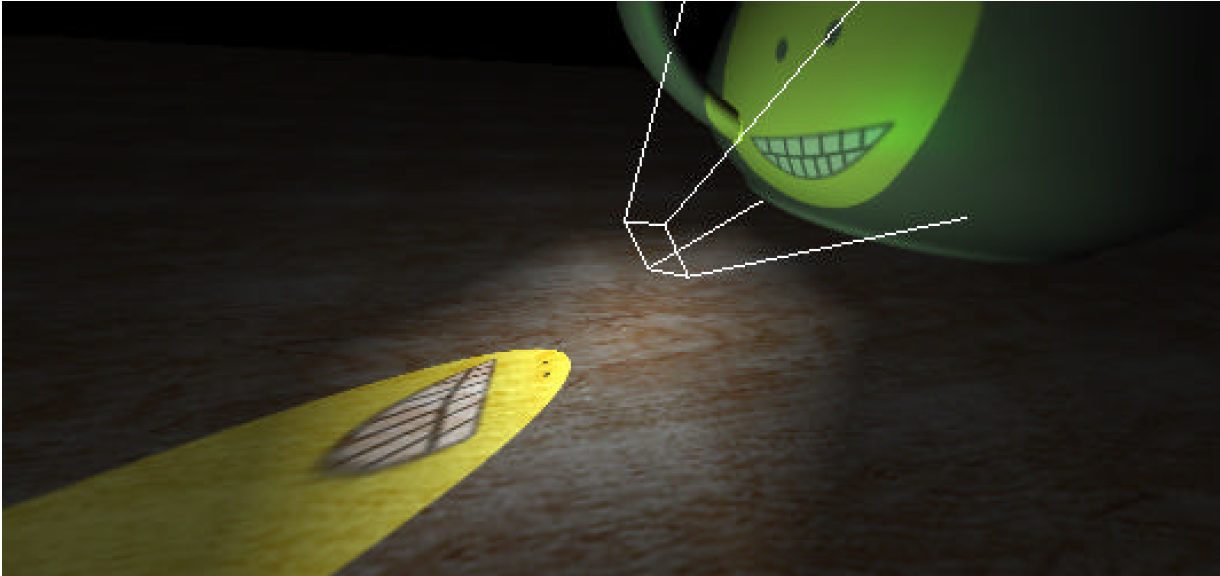
\includegraphics[width=0.85\textwidth]{figures/ReverseProjecton.PNG}
    \caption{Reverse projection after applying PTM. Courtesy of \cite{cassNvidia}}
    \label{fig:ReverseProjection}
\end{figure}

\subsubsection{Results}

In addition to what has been described, a frustum has also been created for debugging purposes, so that we can see the virtual projector in the scene. The full code of the projective texture mapping shaders(for shaded scenes), is available in a \textit{stackoverflow} discussion(available at \cite{avram2014}). I originally started it, while I was stuck on this problem. The previous resource may also describe some aspects in greater detail. The algorithm has been applied on several objects in figure \ref{fig:PTMTest}. Further, in the accompanying thesis video(see appendix \ref{appendix:A}), there is another example of the projected texture being moved, by transforming the virtual slide projector.

\begin{figure}[hbtp]
    \centering
    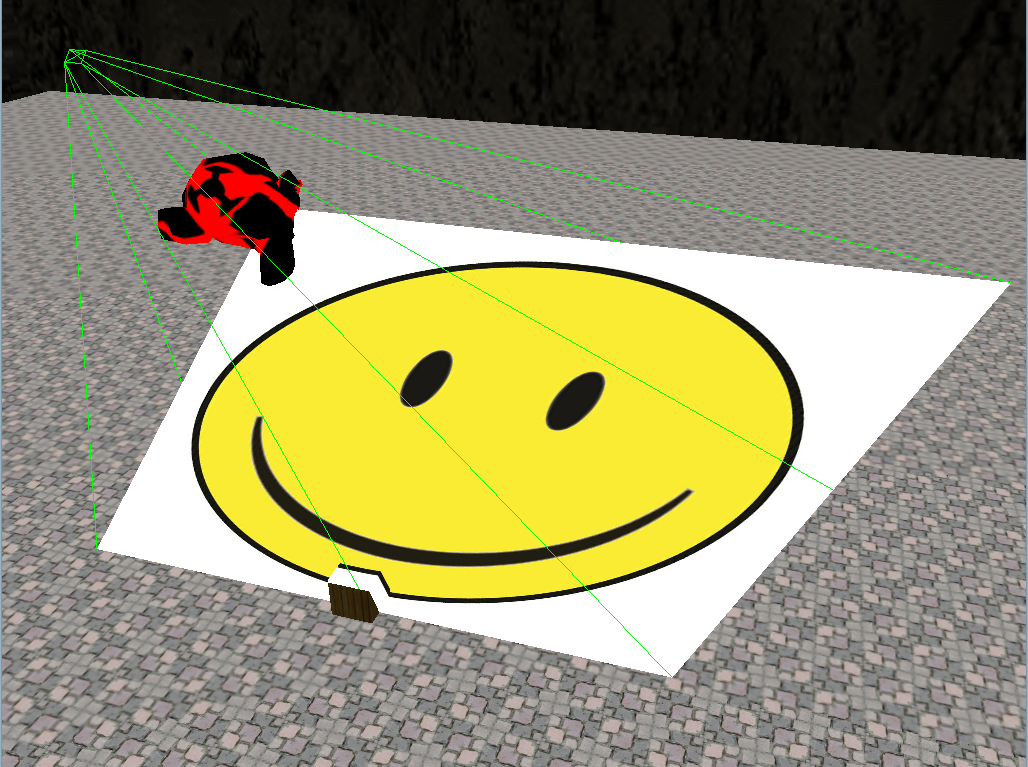
\includegraphics[width=0.85\textwidth]{figures/PTMTest.png}
    \caption{PTM applied on a Suzanne monkey head from Blender, and on a floor with a small cube. The frustum represents the virtual projector.}
    \label{fig:PTMTest}
\end{figure}

Further more, the \verb|debug| flag was used later on in order to change the color of the vertices, if they are within a certain depth range.


\subsection{Manual System Alignment (Calibration Not Used)}
\label{sec:ManualAlignment}

A manual alignment of the components has been employed, due to timing restrictions(the attempted calibration methods did not work). The results are not as precise as with regular calibration, and an extension to this project would be to correctly calibrate the projector-(depth)camera system. In this section I will outline the main steps and tests needed in order to make sure that the alignment is acceptable.

\subsubsection{Physical Projector Alignment to the Physical Screen(Cloth area)}

This step consisted of physically moving the display, positioning it, changing lens shift amounts, using keystone correction etc. In order to test this step, I have created a texture with a grid(see figure \ref{fig:CalibrationGrid}), four colored corners and a red border. The grid and the corners were used to roughly position the projector so that the cloth display is correctly in view. The border was used for some fine tuning. 

\begin{figure}[hbtp]
    \centering
    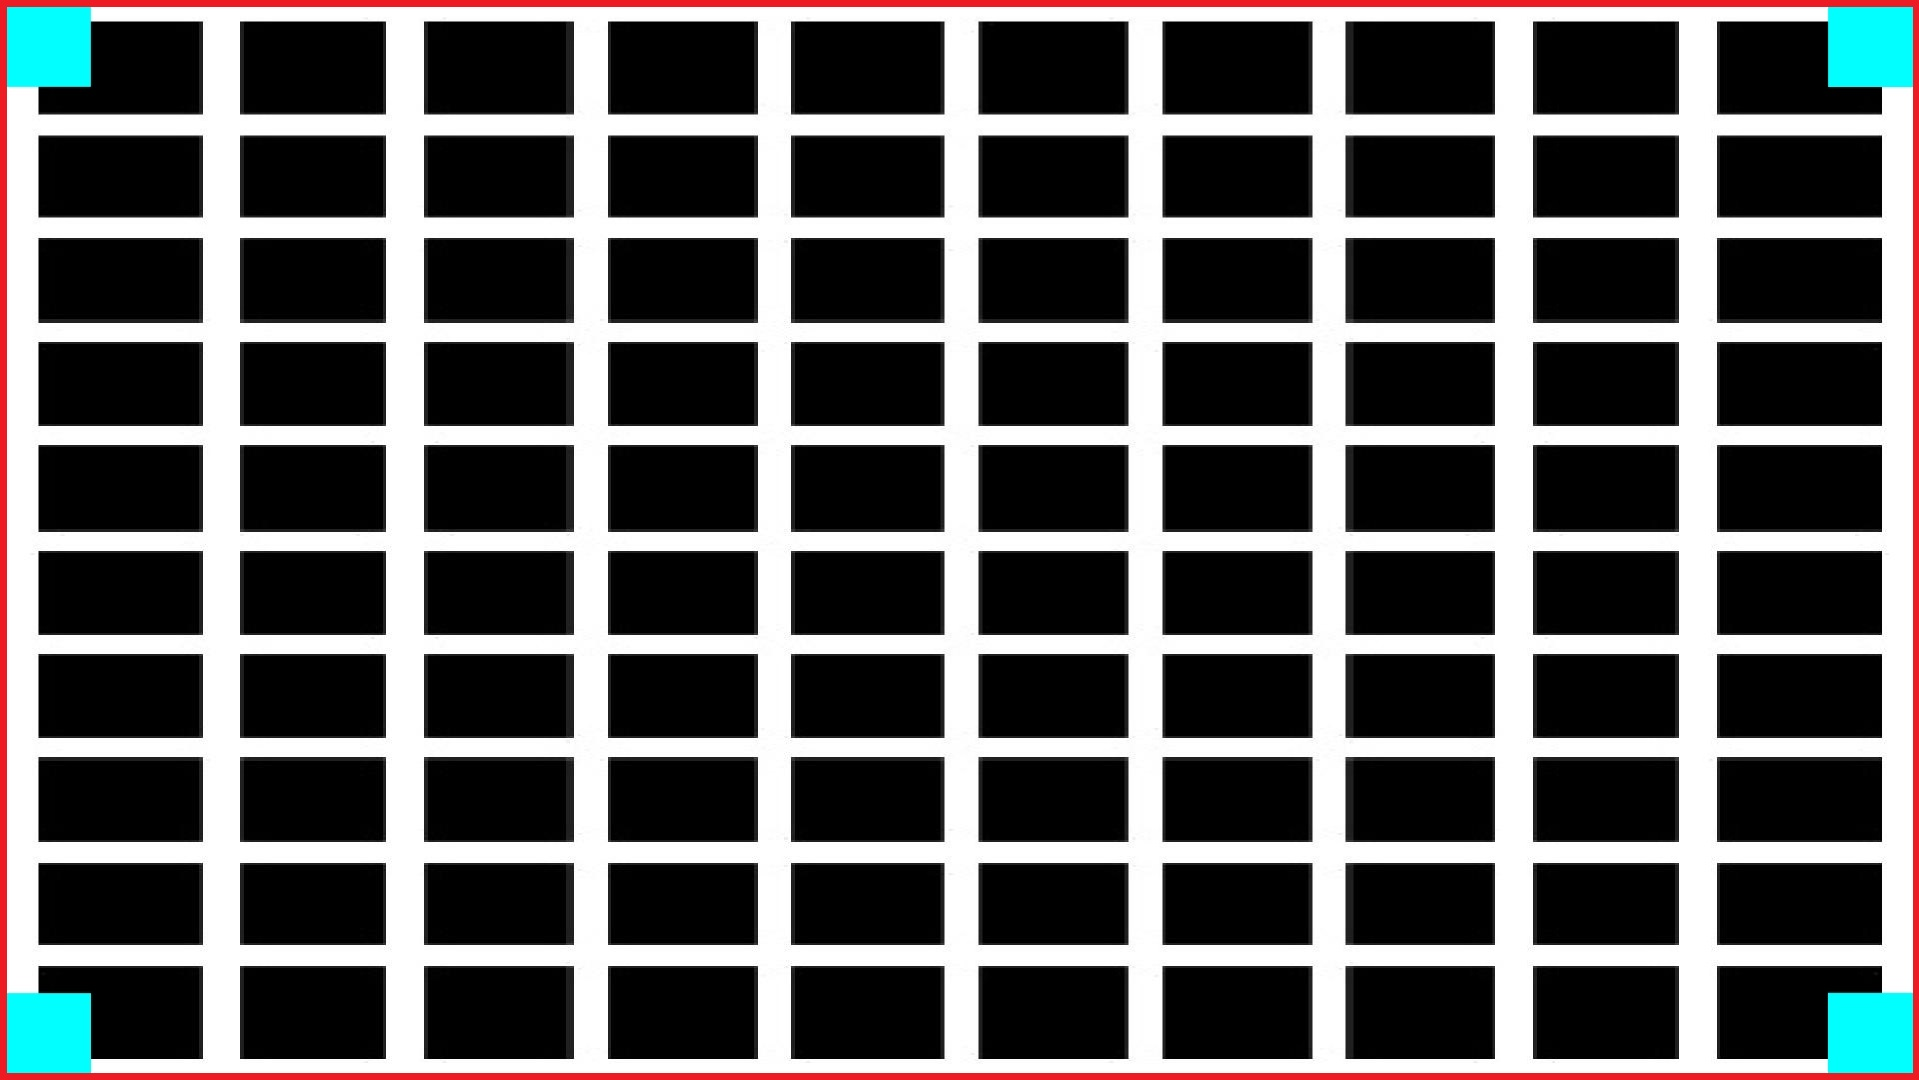
\includegraphics[width=0.85\textwidth]{figures/CalibrationGrid.jpg}
    \caption{A grid with four corners and a red border, used to test the physical alignment of the projector to the cloth.}
    \label{fig:CalibrationGrid}
\end{figure}

Some photo shots were taken, in order to show how well figure \ref{fig:CalibrationGrid} fits the cloth area. The whole surface is shown in figure \ref{fig:ProjectedCalibrationGrid}. In this figure, we can see that the image very closely matches the surface, and that the four cyan squares in the corners roughly correspond to those of the visible cloth area. However, it is hard to see how well the red border is aligned(it is not very visible in this figure). 

\begin{figure}[hbtp]
    \centering
    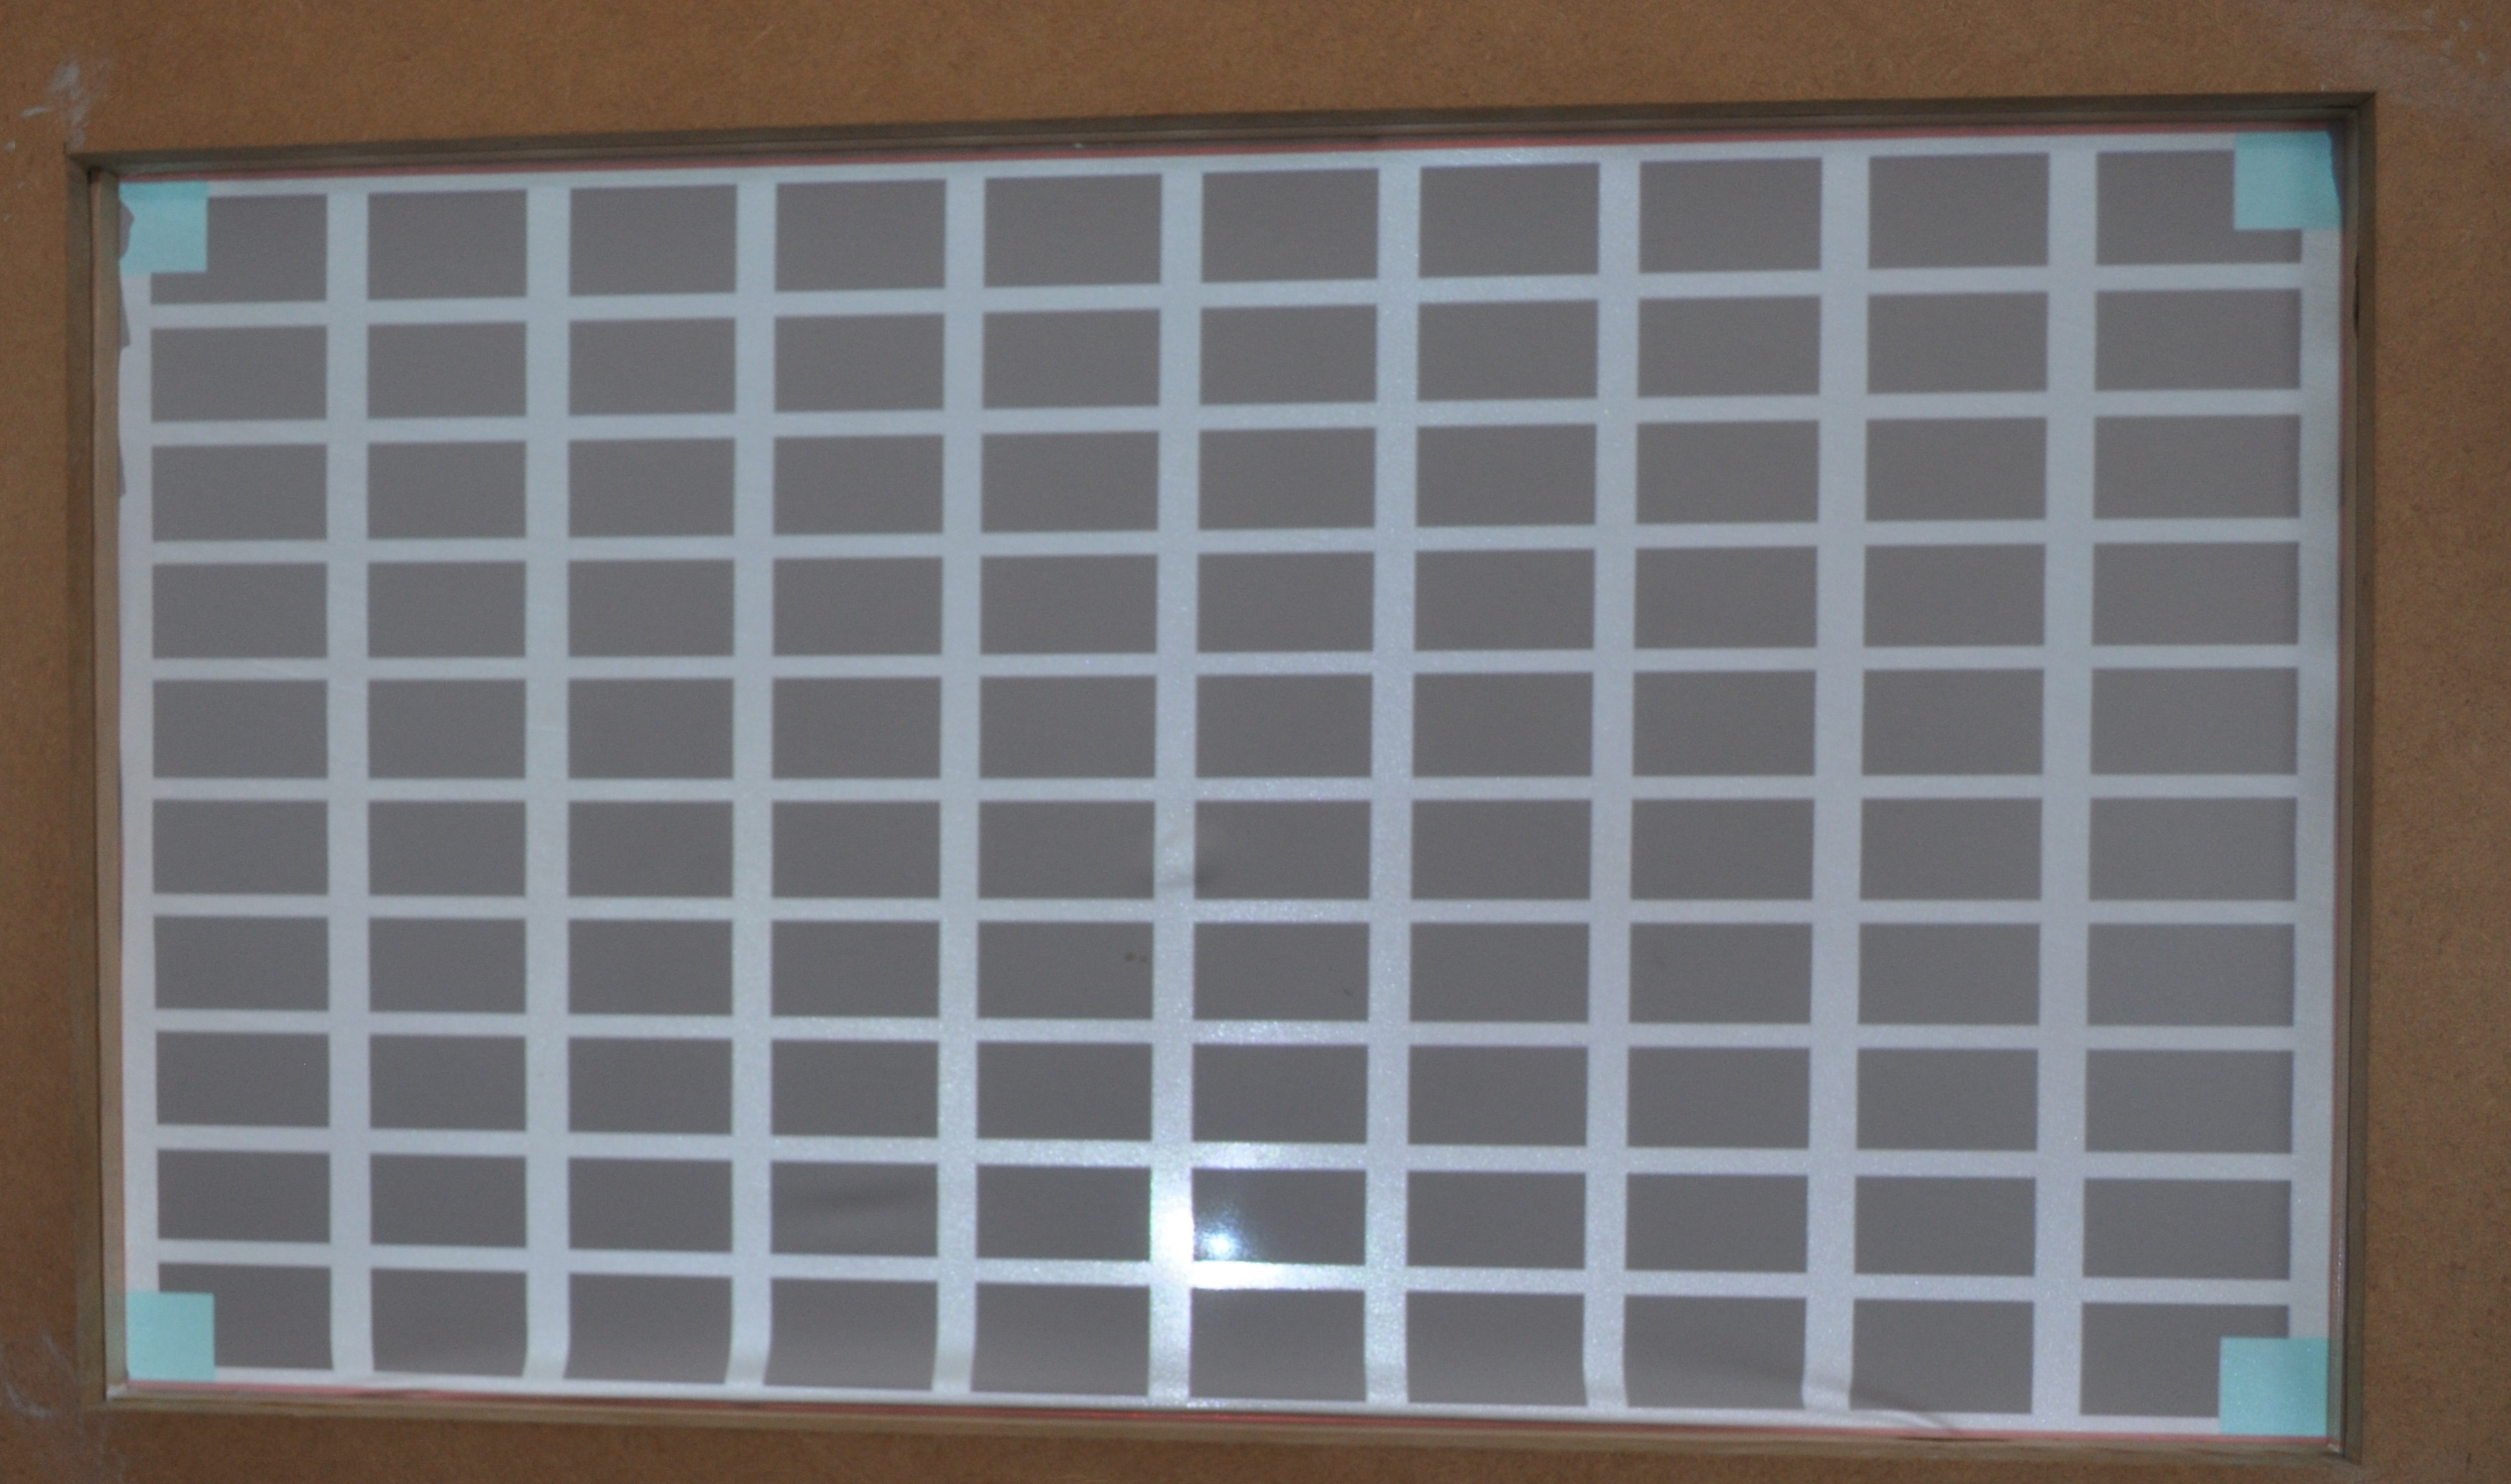
\includegraphics[width=0.85\textwidth]{figures/ProjectedCalibrationGridC2.jpg}
    \caption{The alignment grid texture projected on the cloth.}
    \label{fig:ProjectedCalibrationGrid}
\end{figure}

Some shots of the corners of the frame were taken, so that we can more clearly see how well the grid texture is mapped to the surface. These images are shown in figure \ref{fig:CornerAlignment}.
\begin{figure}[hbtp] 
  \begin{subfigure}[b]{0.5\linewidth}
    \centering
    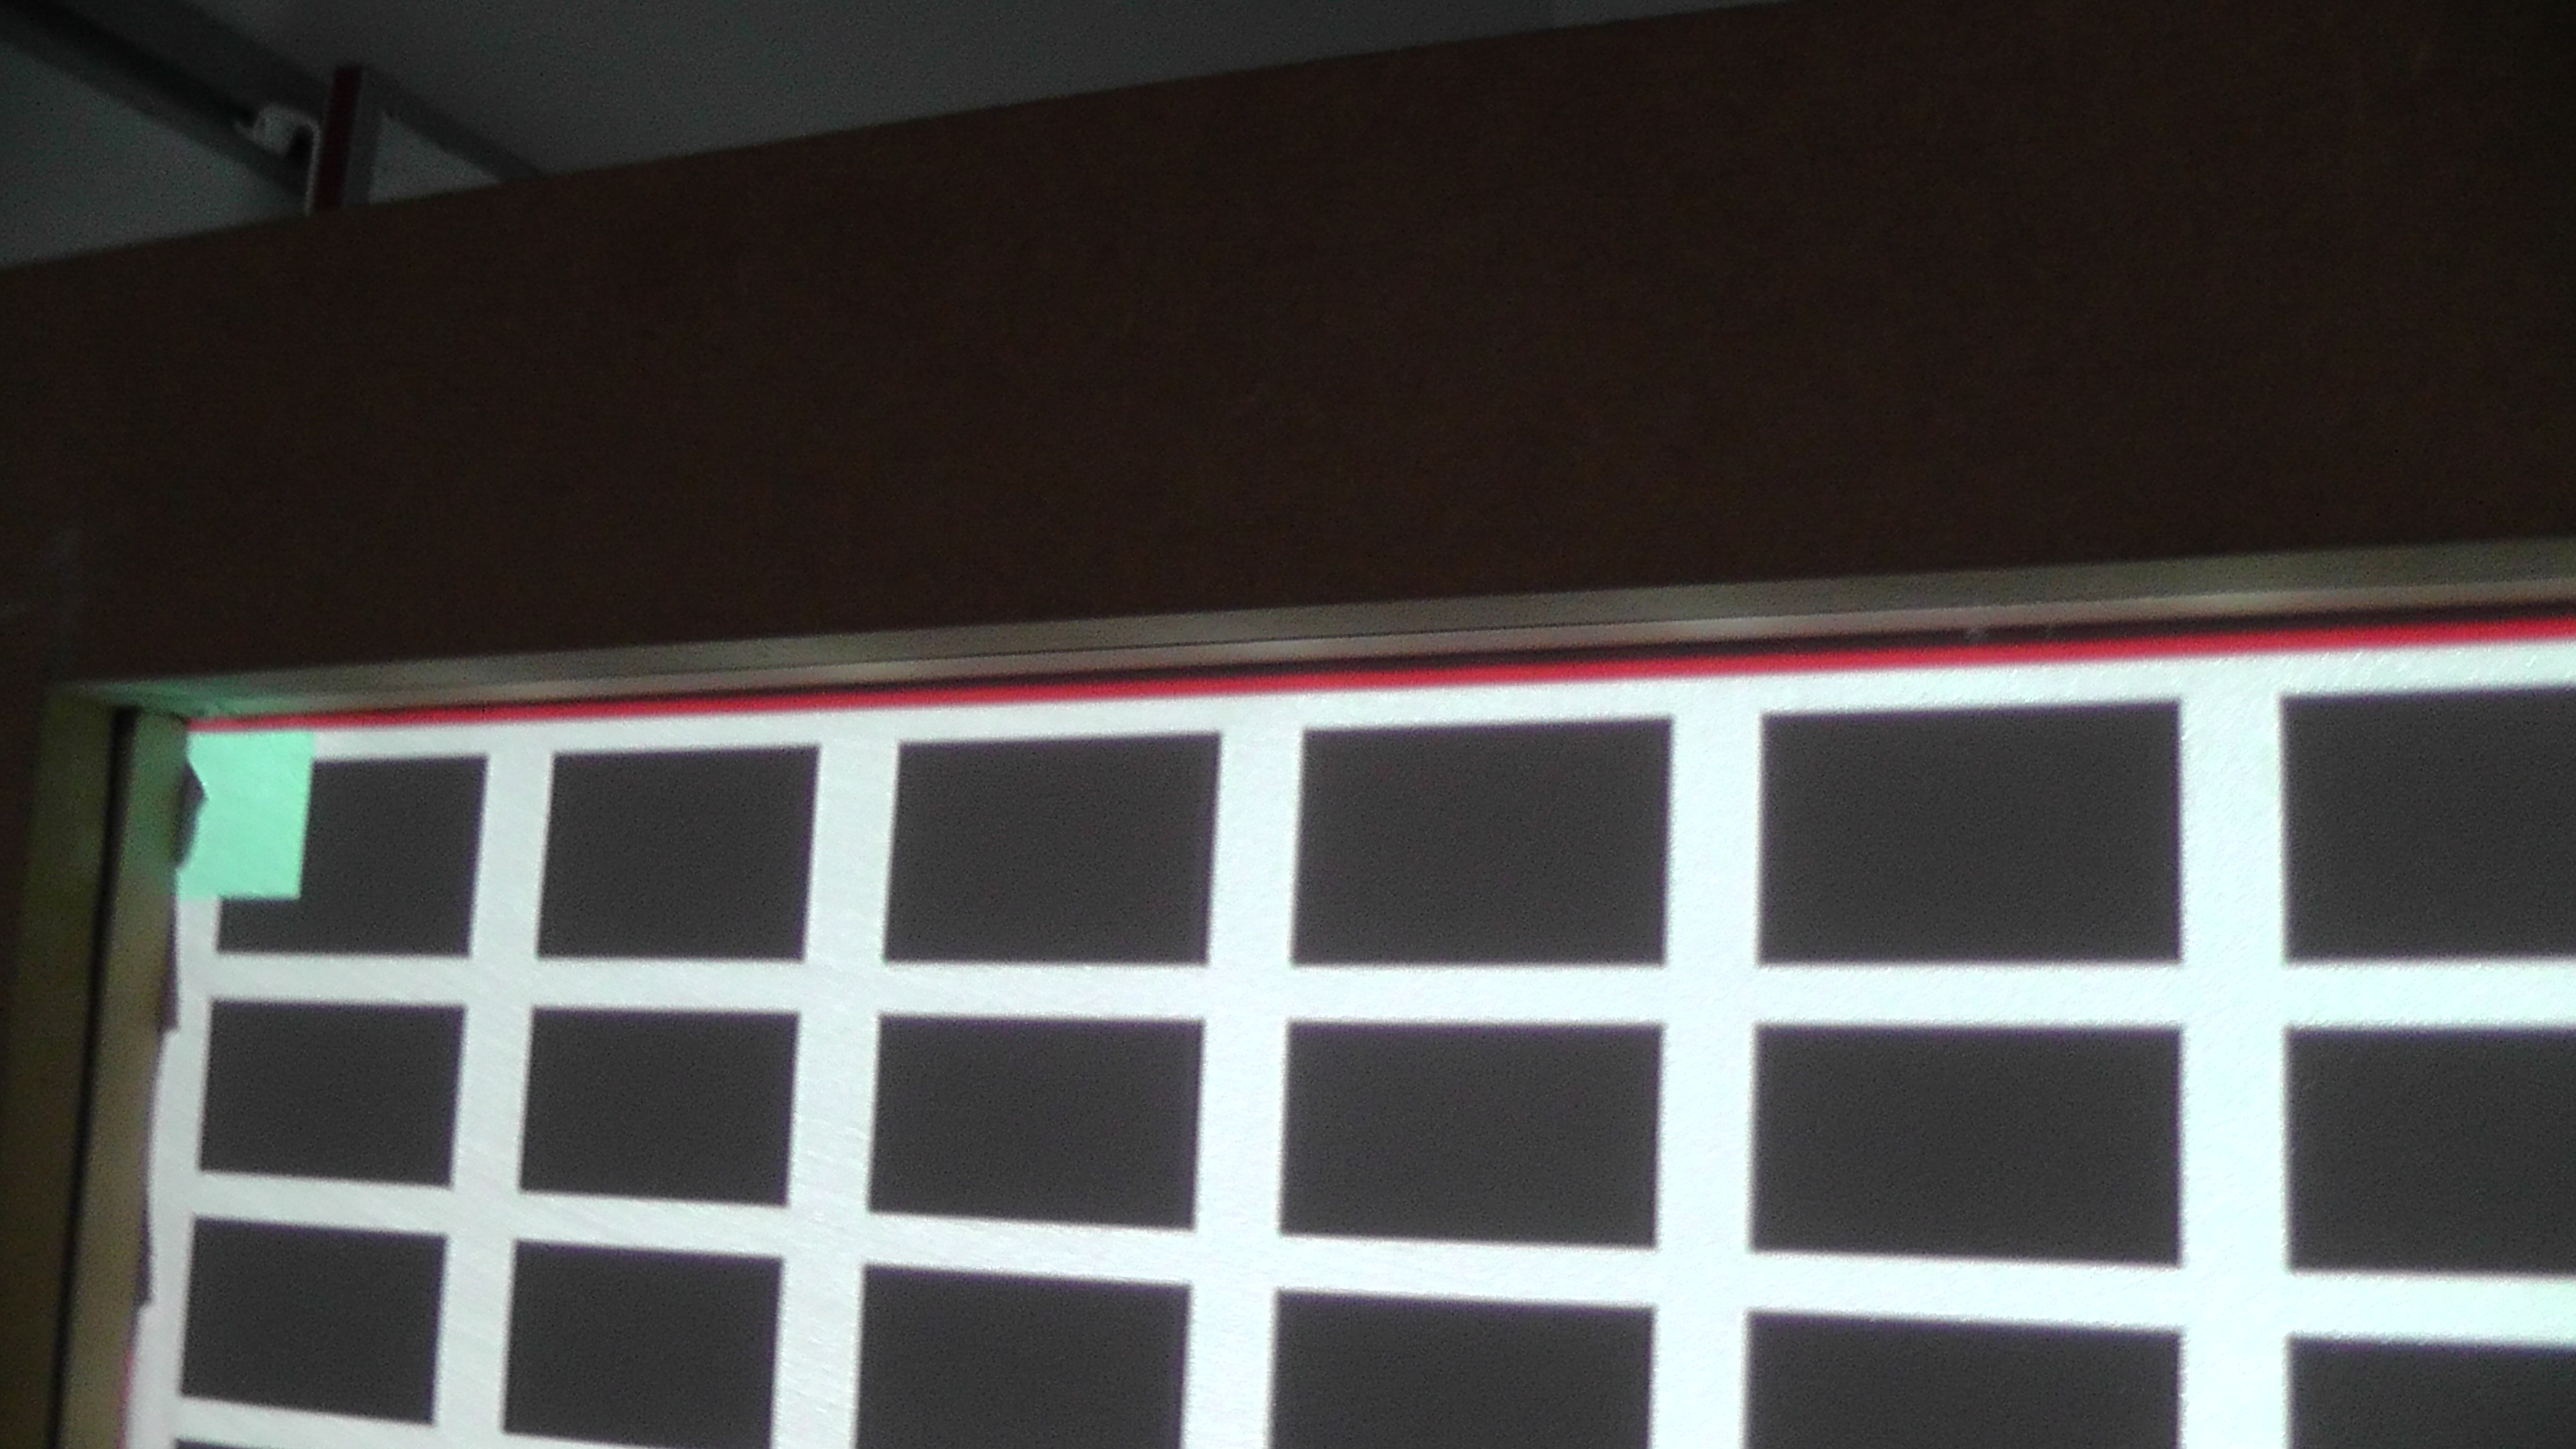
\includegraphics[width=0.75\linewidth]{figures/TopLeft2.JPG} 
    \caption{Top Left Alignment} 
    \label{fig:TLA} 
    \vspace{4ex}
  \end{subfigure}%% 
  \begin{subfigure}[b]{0.5\linewidth}
    \centering
    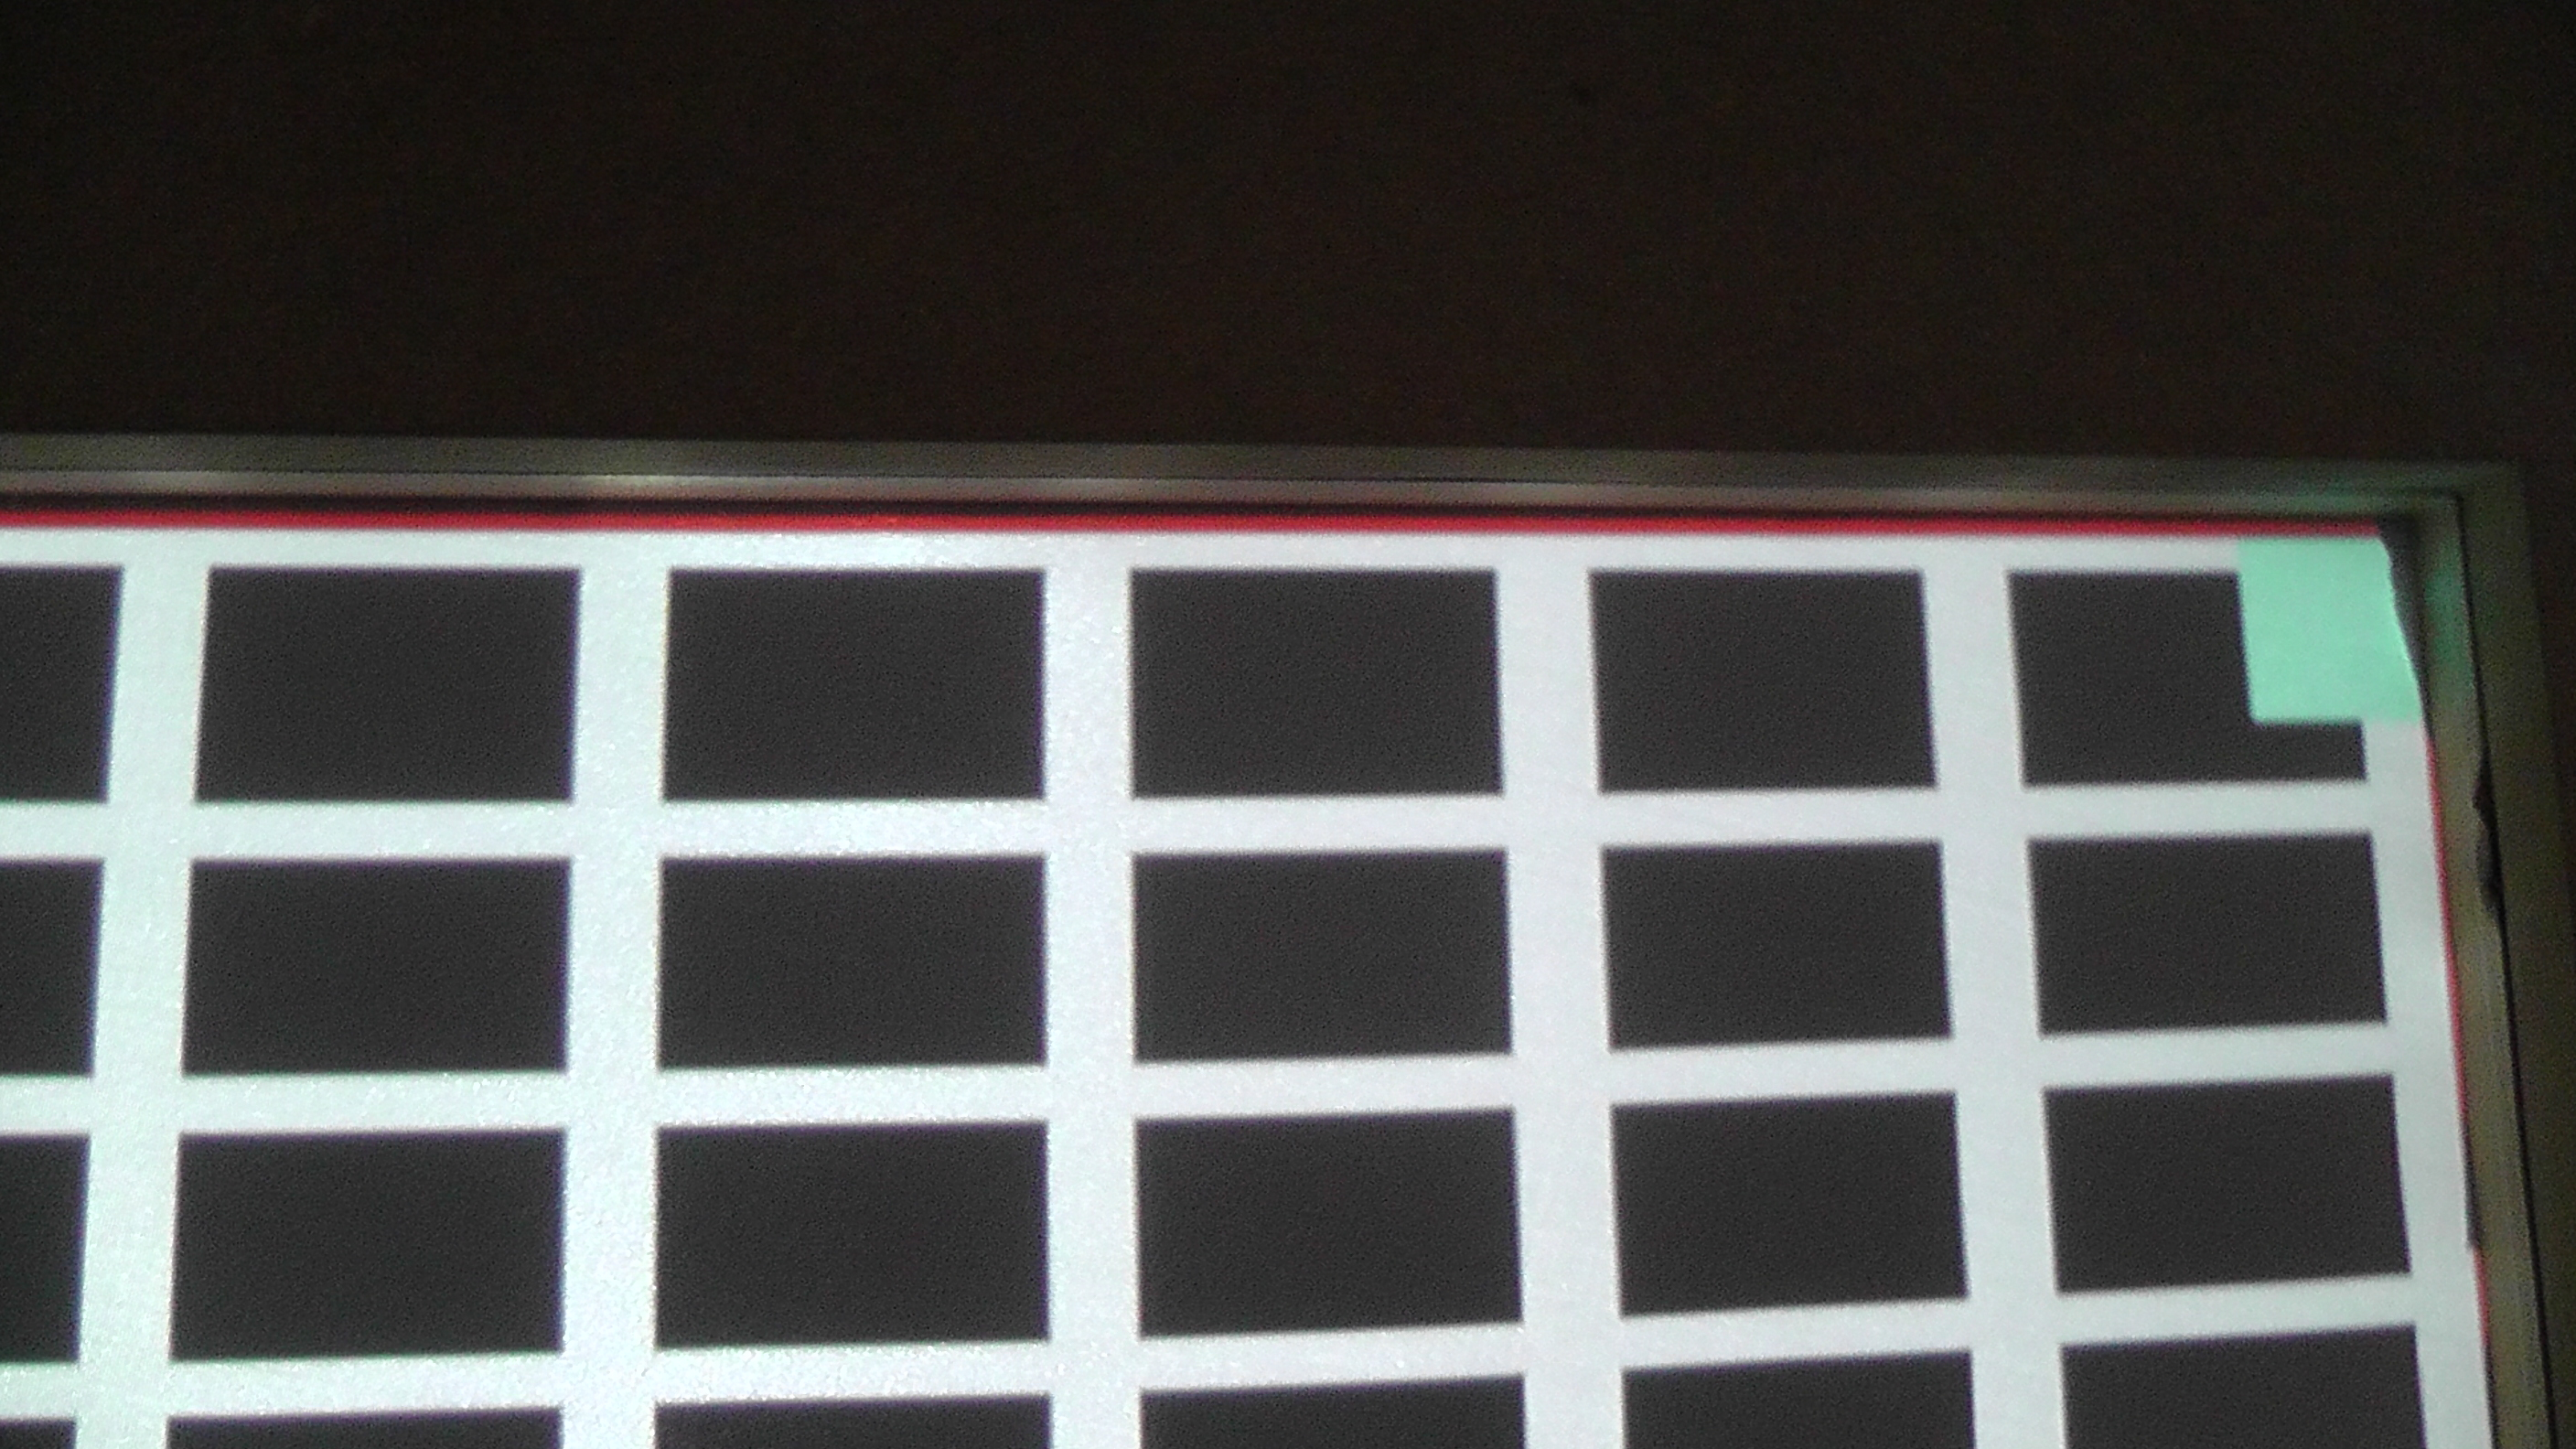
\includegraphics[width=0.75\linewidth]{figures/TopRight.JPG} 
    \caption{Top Right Alignment} 
    \label{fig:TRA} 
    \vspace{4ex}
  \end{subfigure} 
  \begin{subfigure}[b]{0.5\linewidth}
    \centering
    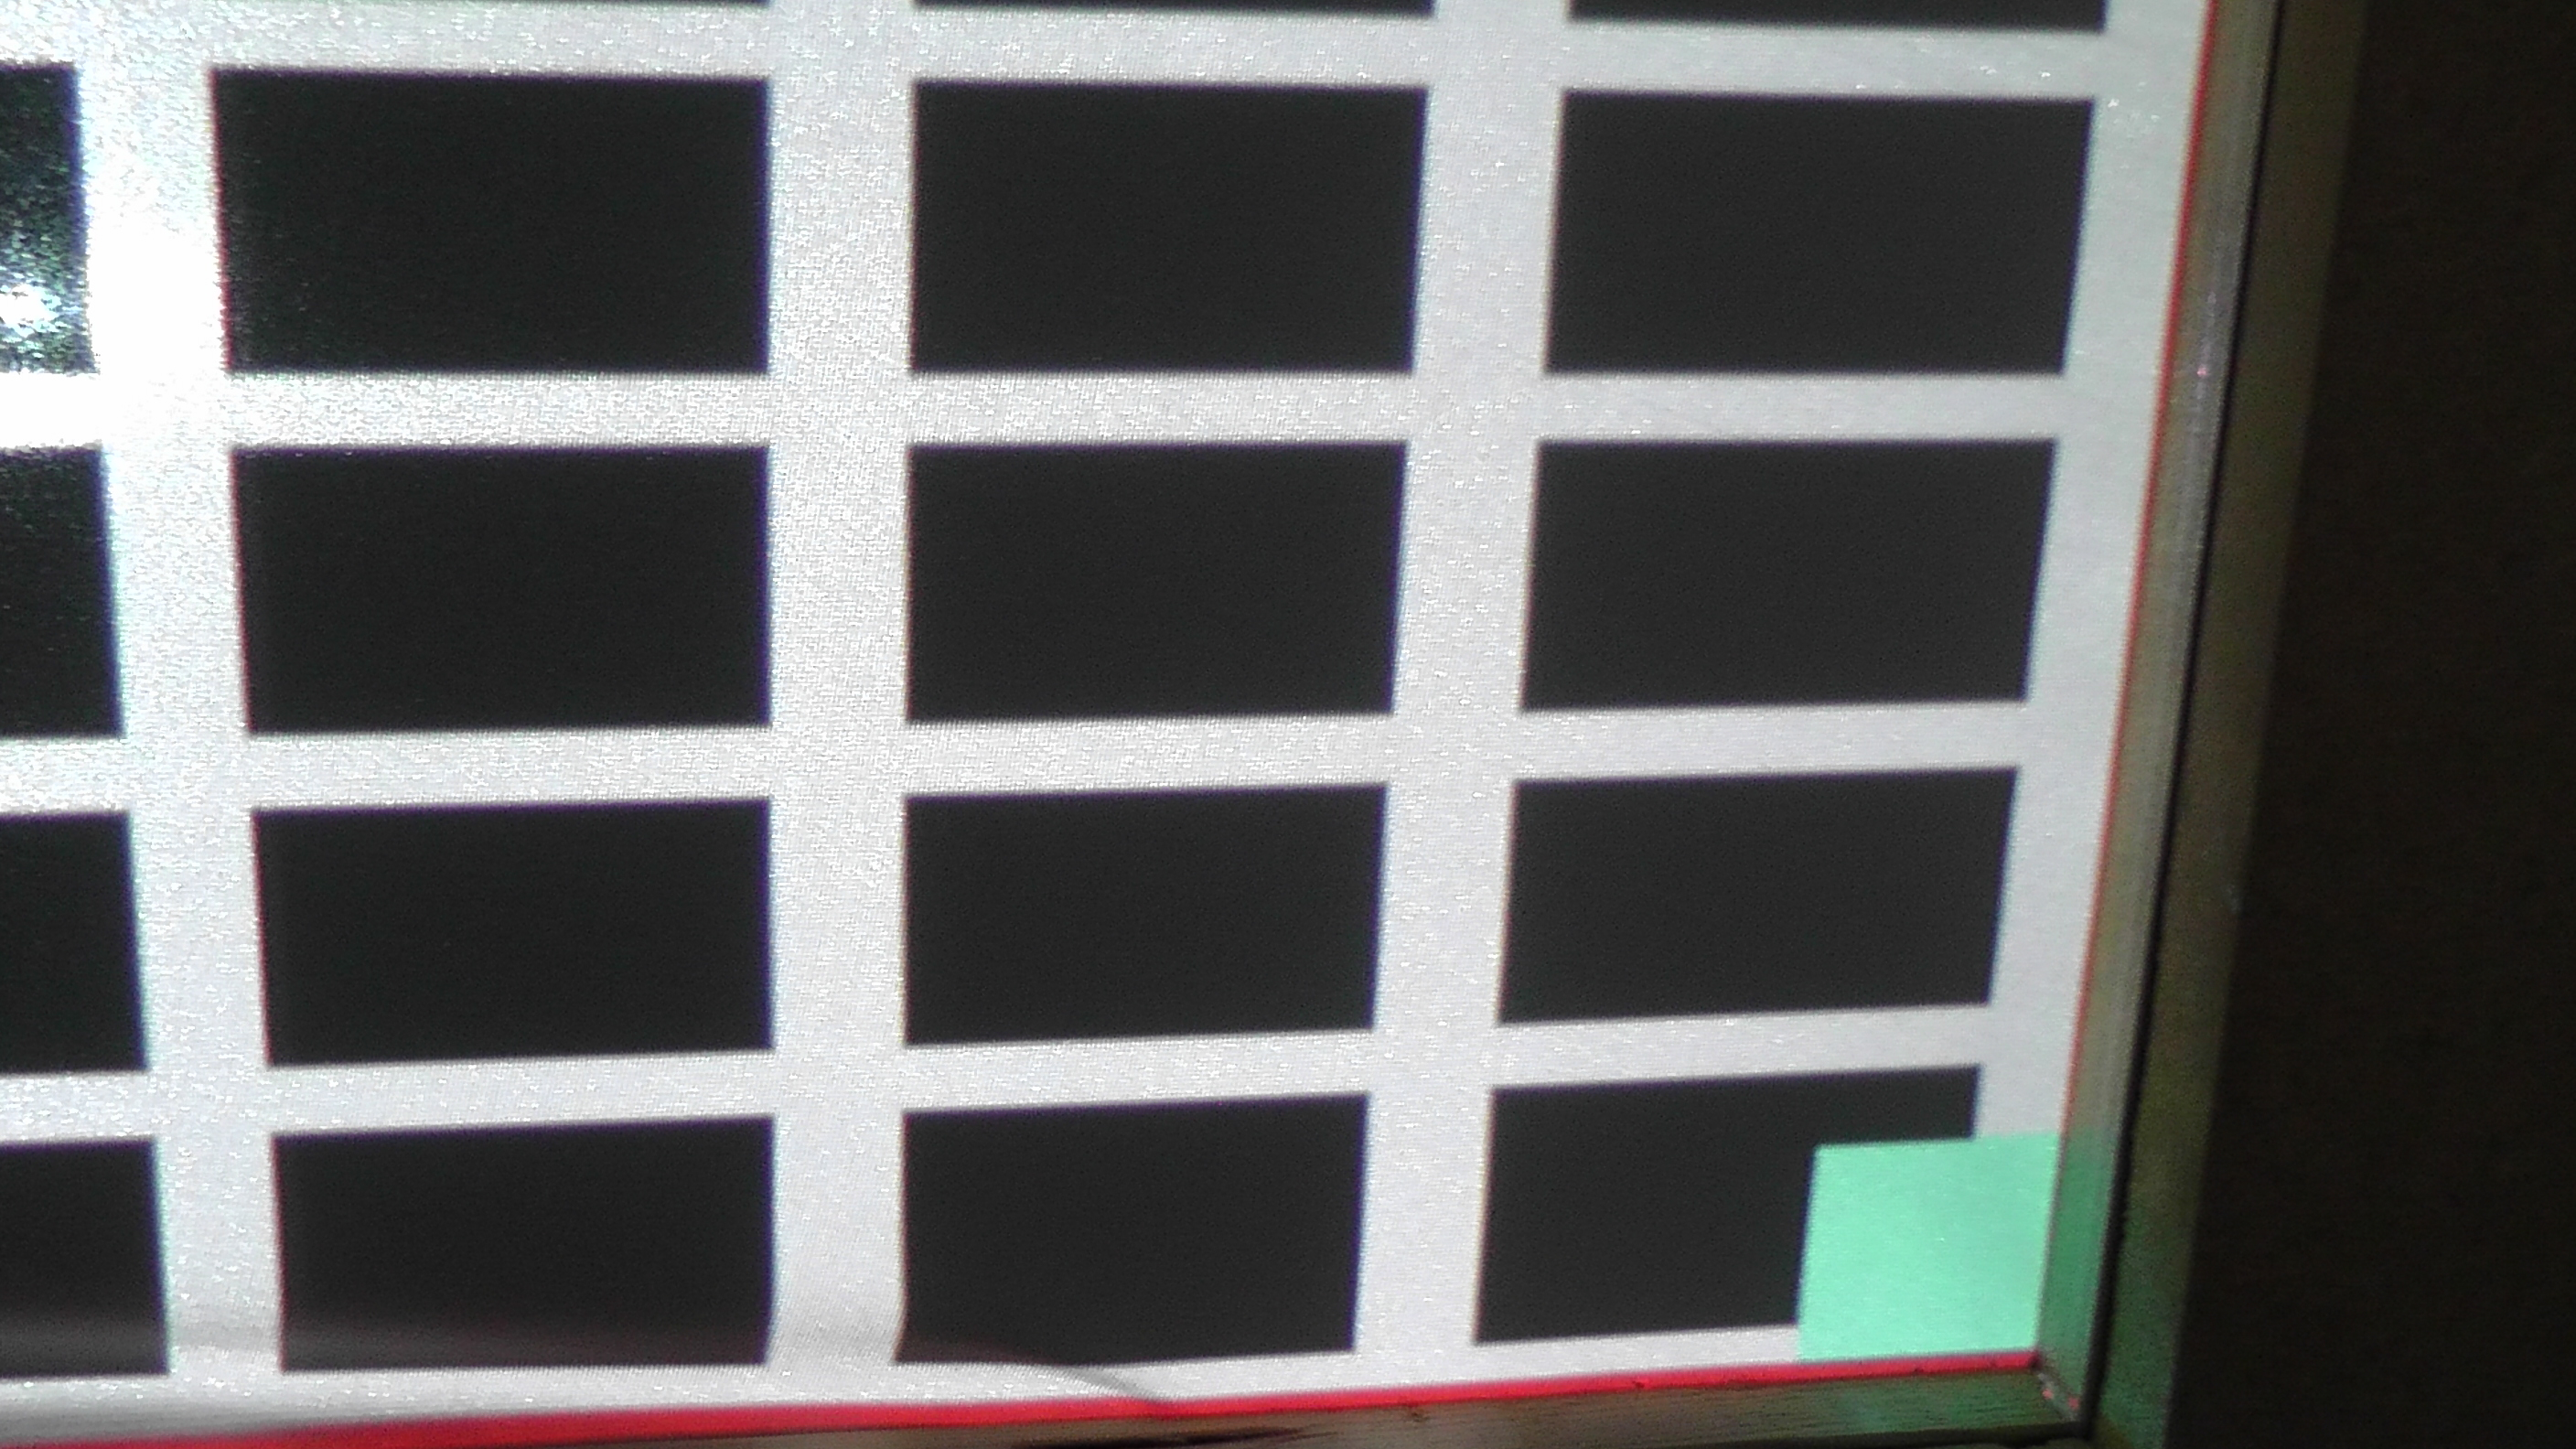
\includegraphics[width=0.75\linewidth]{figures/BottomRight.JPG} 
    \caption{Bottom Right Alignment} 
    \label{fig7:BRA} 
  \end{subfigure}%%
  \begin{subfigure}[b]{0.5\linewidth}
    \centering
    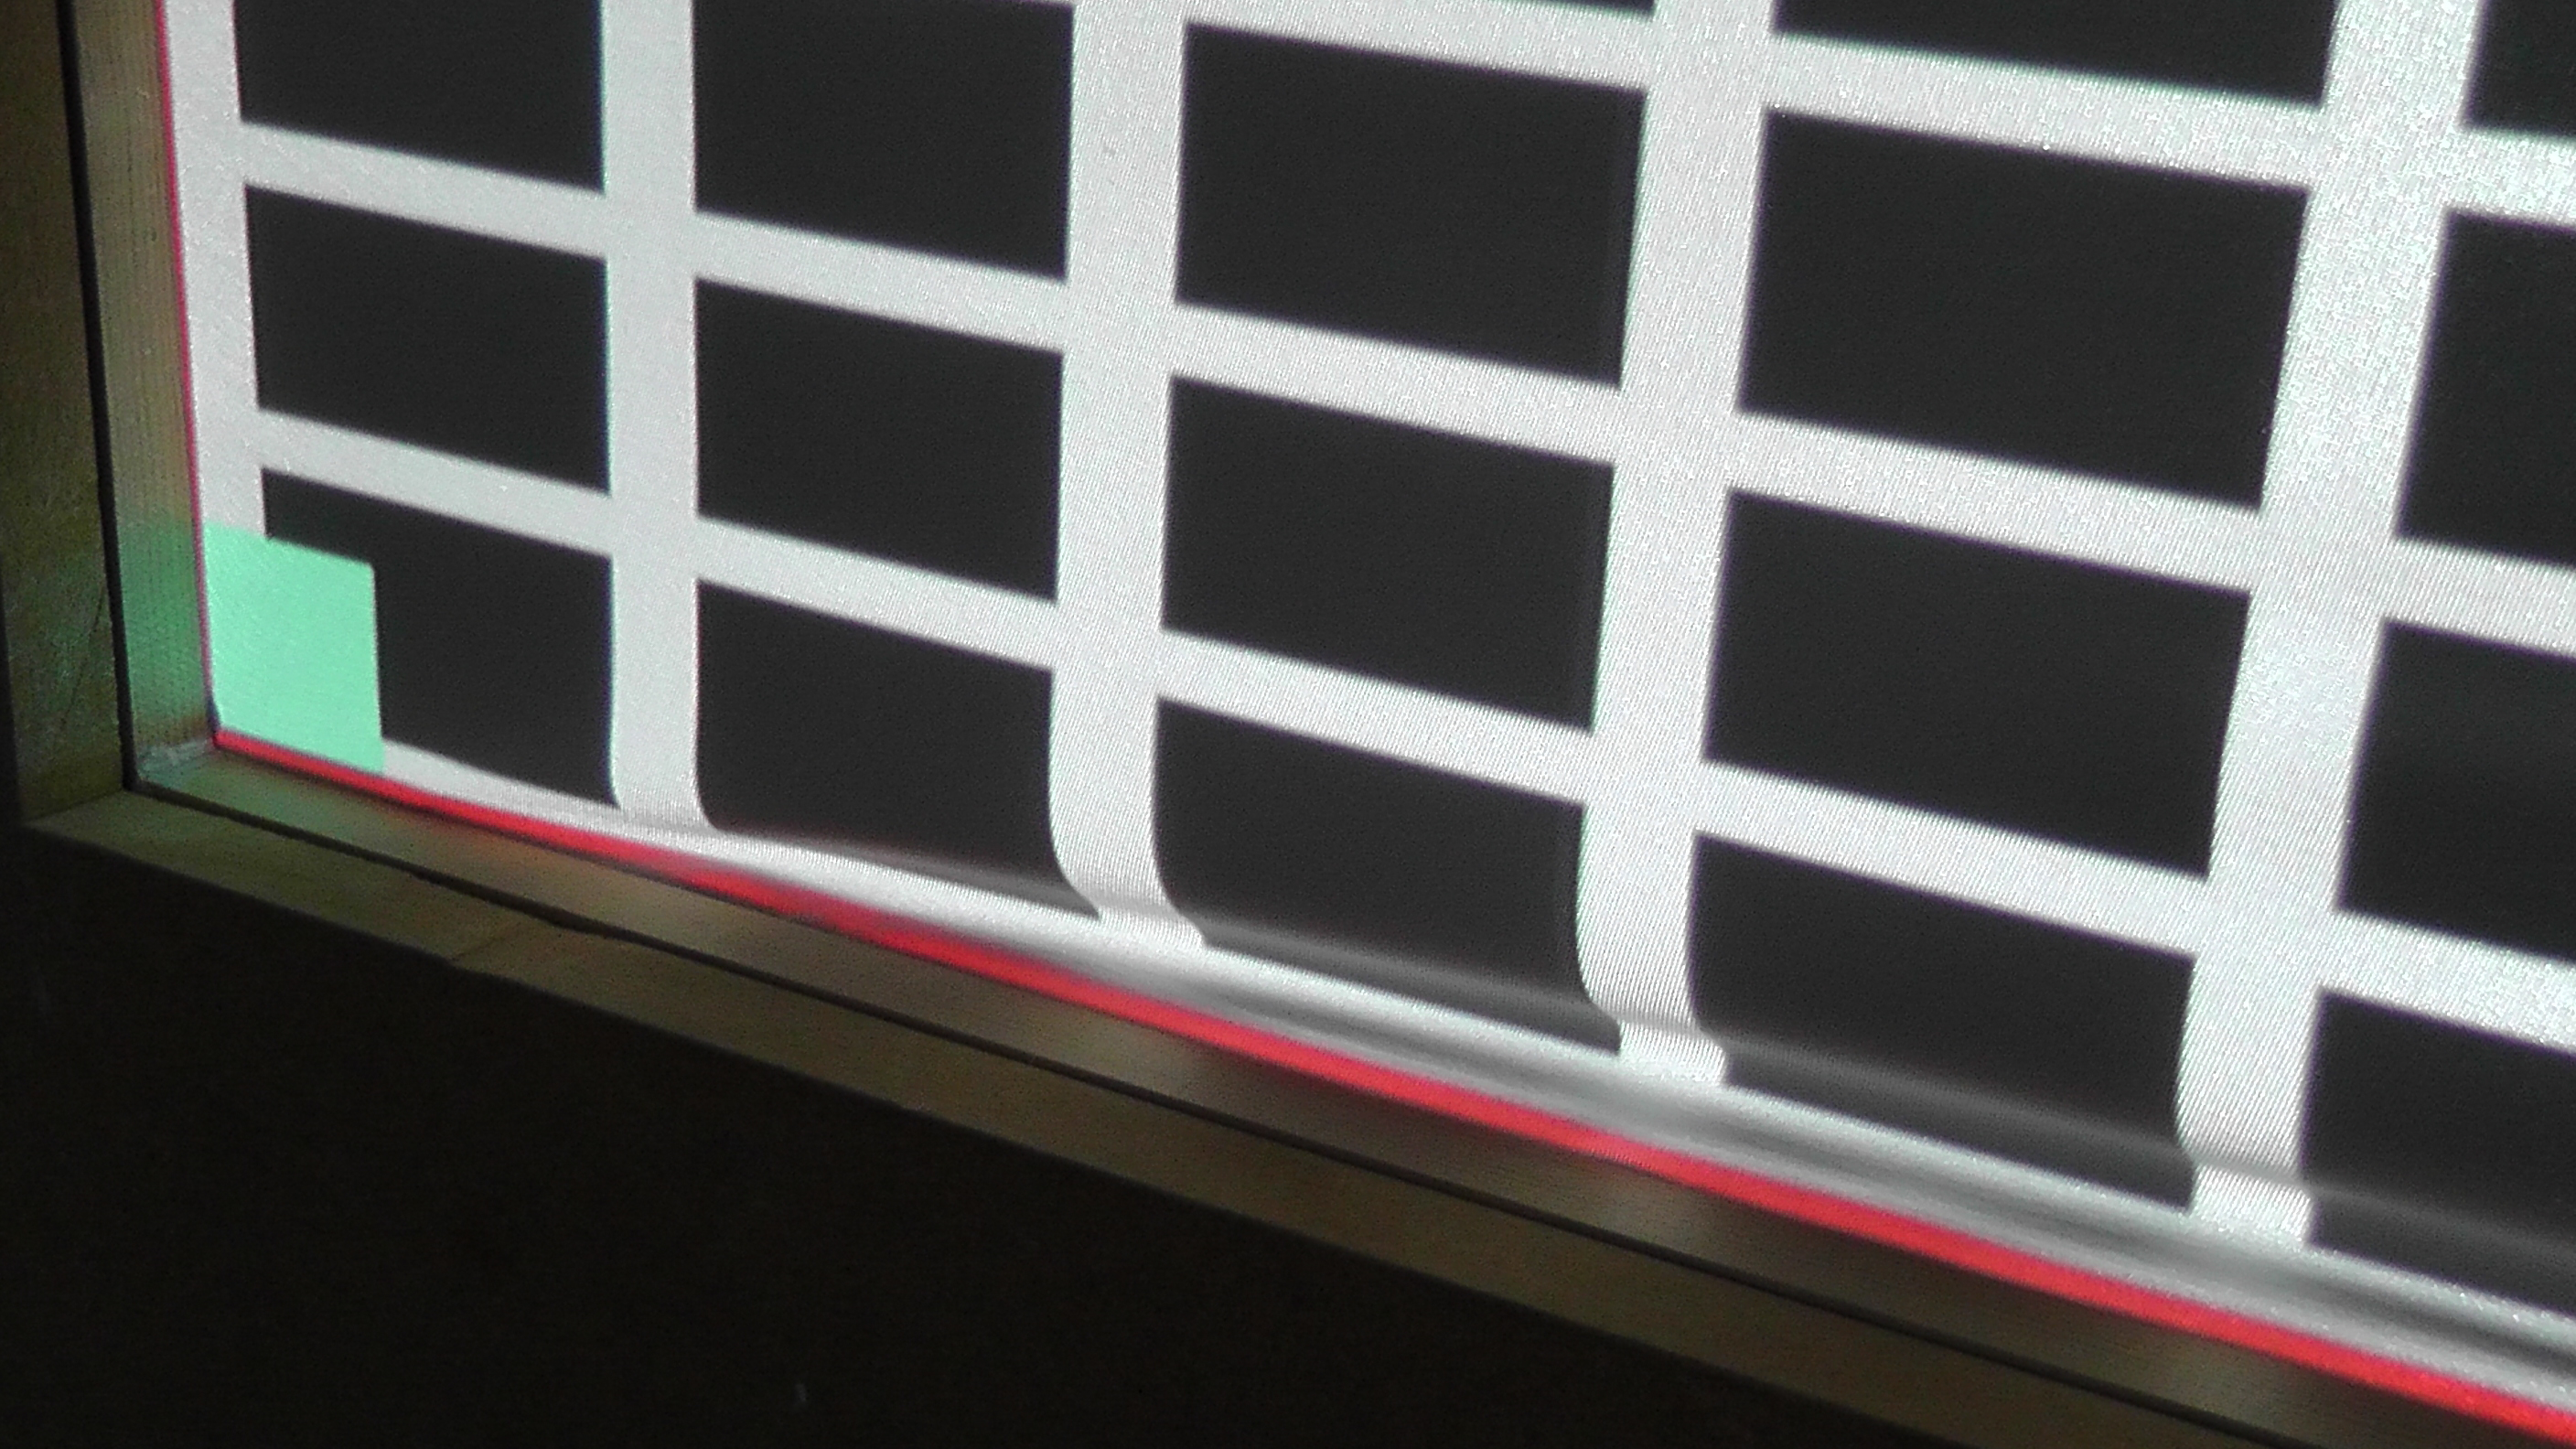
\includegraphics[width=0.75\linewidth]{figures/BottomLeft2.JPG} 
    \caption{Bottom Left Alignment} 
    \label{fig7:BLA} 
  \end{subfigure} 
  \caption{Illustration of alignments in the four corners of the frame.}
  \label{fig:CornerAlignment} 
\end{figure}

 From these images, we can see that the texture is reasonably well aligned, but the red borders are not very visible on the sides, and the image is slightly skewed towards the upper left, making the border disappear completely in that part of the image. Some space is also present in the upper central area. This may be due to the cloth not being perfectly flat. Some of these visual cues may be hard to spot on these figures, so they will be also displayed in appendix \ref{appendix:B-alignment}, in a larger size.

\subsubsection{Physical Depth Camera Alignment to the Physical Screen (Cloth area)}

The depth camera was also aligned to the cloth manually, by trial and error. The objective was to position the camera as orthogonal as possible onto the cloth display. In order to do this physically, I used a tripod with the camera attached upside down, to an inverse tripod column(see the setup in figure \ref{fig:Tripod}). 

\begin{figure}[hbtp]
    \centering
    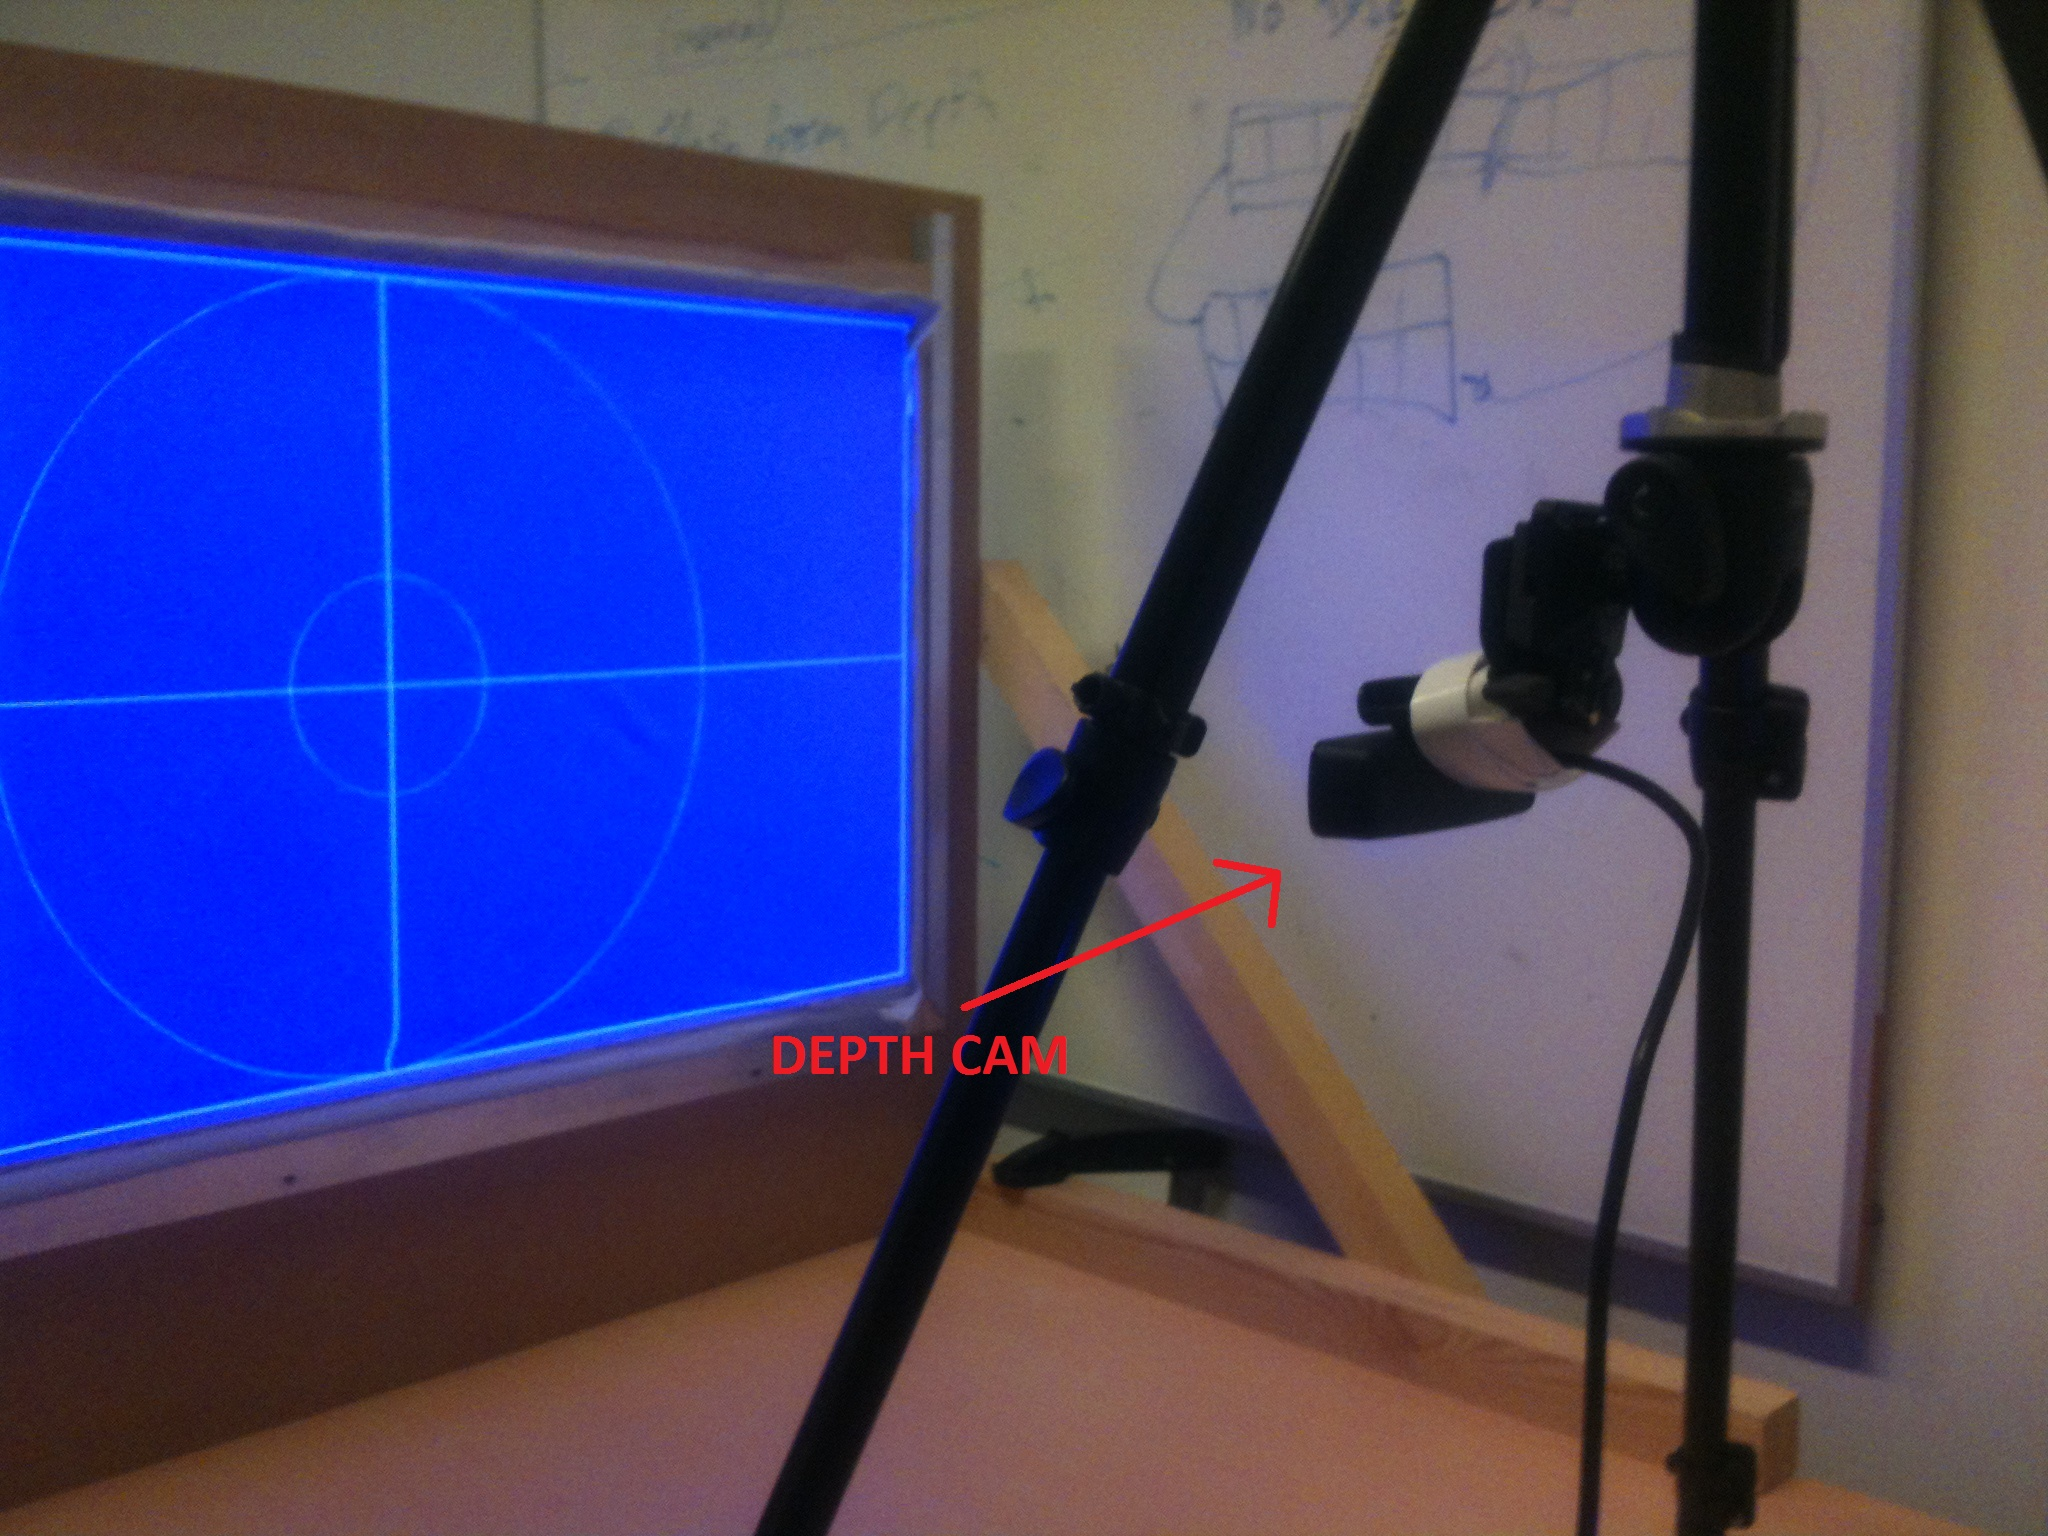
\includegraphics[width=0.7\textwidth]{figures/tripodCamSetup.jpg}
    \caption{The depth camera is setup on a tripod. By reversing the column we can get the center of the depth camera to roughly correspond to the center of the projected image.}
    \label{fig:Tripod}
\end{figure}

This setup allowed to position the camera fairly close to the screen and fairly straight on. It has been tested by displaying a pattern on the projector and touching the center, while observing the corresponding changes in the depth stream. As you can see in figure \ref{fig:CenterPointAlignment}, the point is roughly in the middle of both images.

\begin{figure}
\centering
\begin{subfigure}{.5\textwidth}
  \centering
  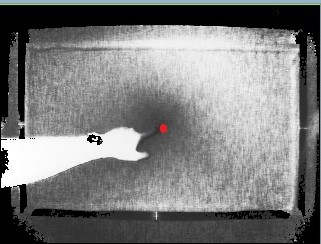
\includegraphics[width=0.9\linewidth]{figures/DepthStreamCenterPoint.jpg}
  \caption{Depth Stream Center Point}
  \label{fig:DepthStreamCenterPoint}
\end{subfigure}%
\begin{subfigure}{.5\textwidth}
  \centering
  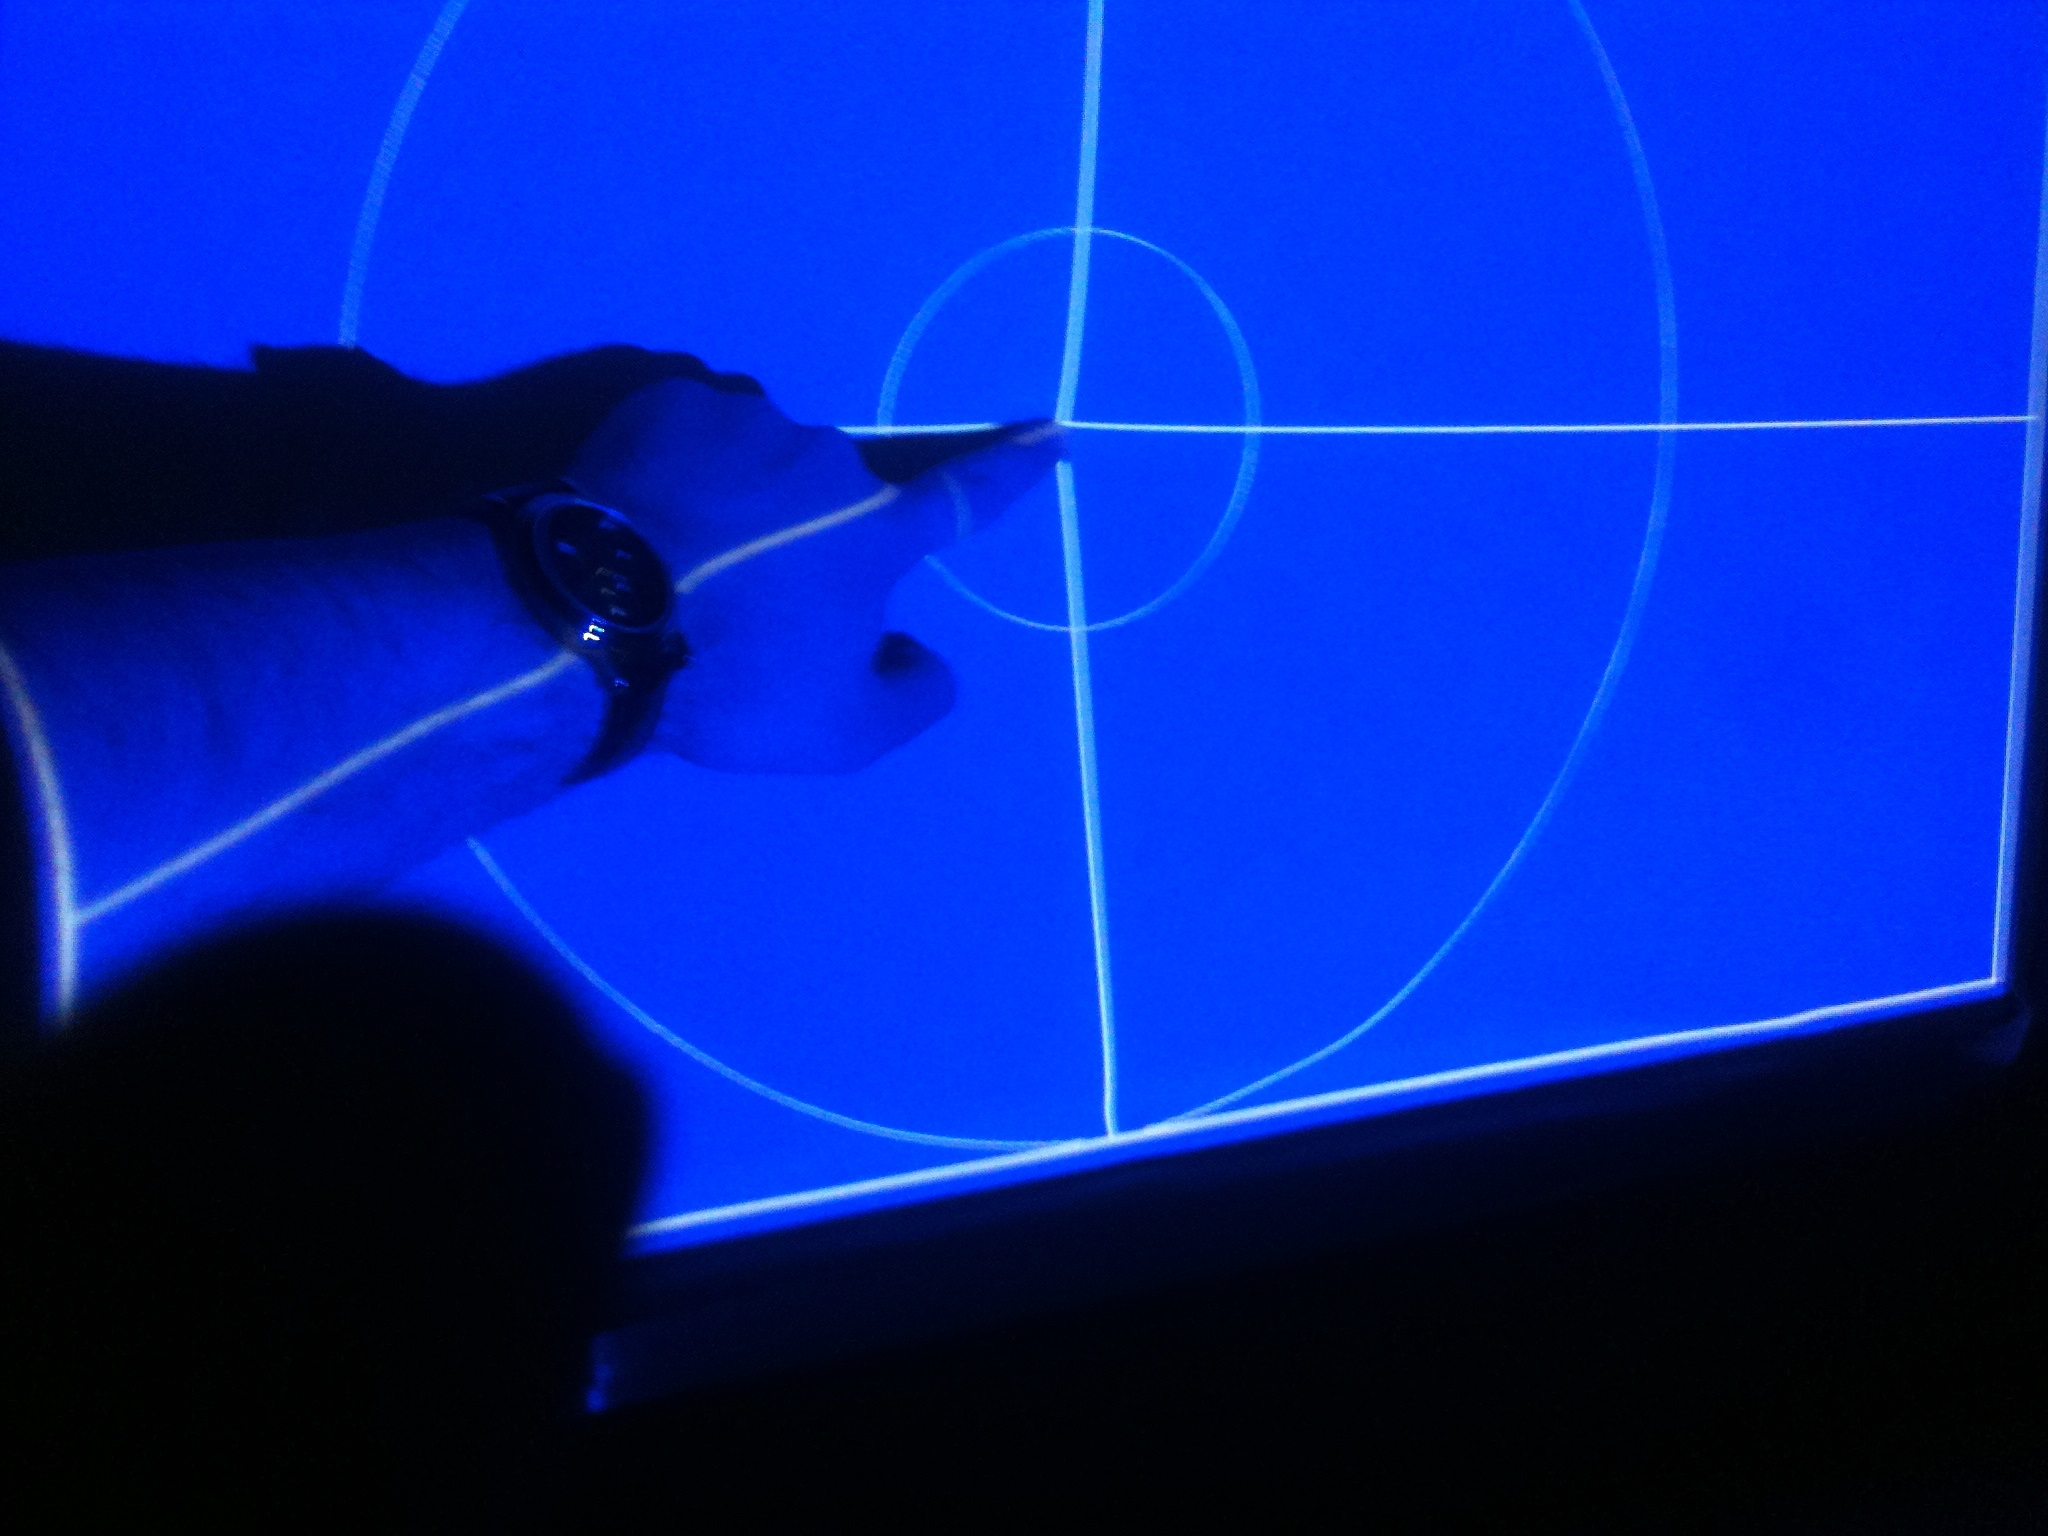
\includegraphics[width=0.9\linewidth]{figures/CenterPointPattern.JPG}
  \caption{Projection Pattern Center Point}
  \label{fig:CenterPointPattern}
\end{subfigure}
\caption{A comparison which shows that pushing in the center roughly modifies the same area of both the depth stream and physical image.}
\label{fig:CenterPointAlignment}
\end{figure}

 However, this figure only provides information about the alignment of the image's center area. In order to test the sides, we can check the depth values of points, in different areas on the screen. Of course, the depth of the captured object has to be the same in the physical world - we can use the wooden frame for this. The frame has been placed at a distance of approximately $2.5$ centimeters from the edge of the desk, as shown in figure \ref{fig:FramePlacement}. However, as you can see, there is a slight offset, with one side being slightly closer to the edge. This issue may also introduce some minor depth discrepancies. 
 
 \begin{figure}[!hbtp]
     \centering
     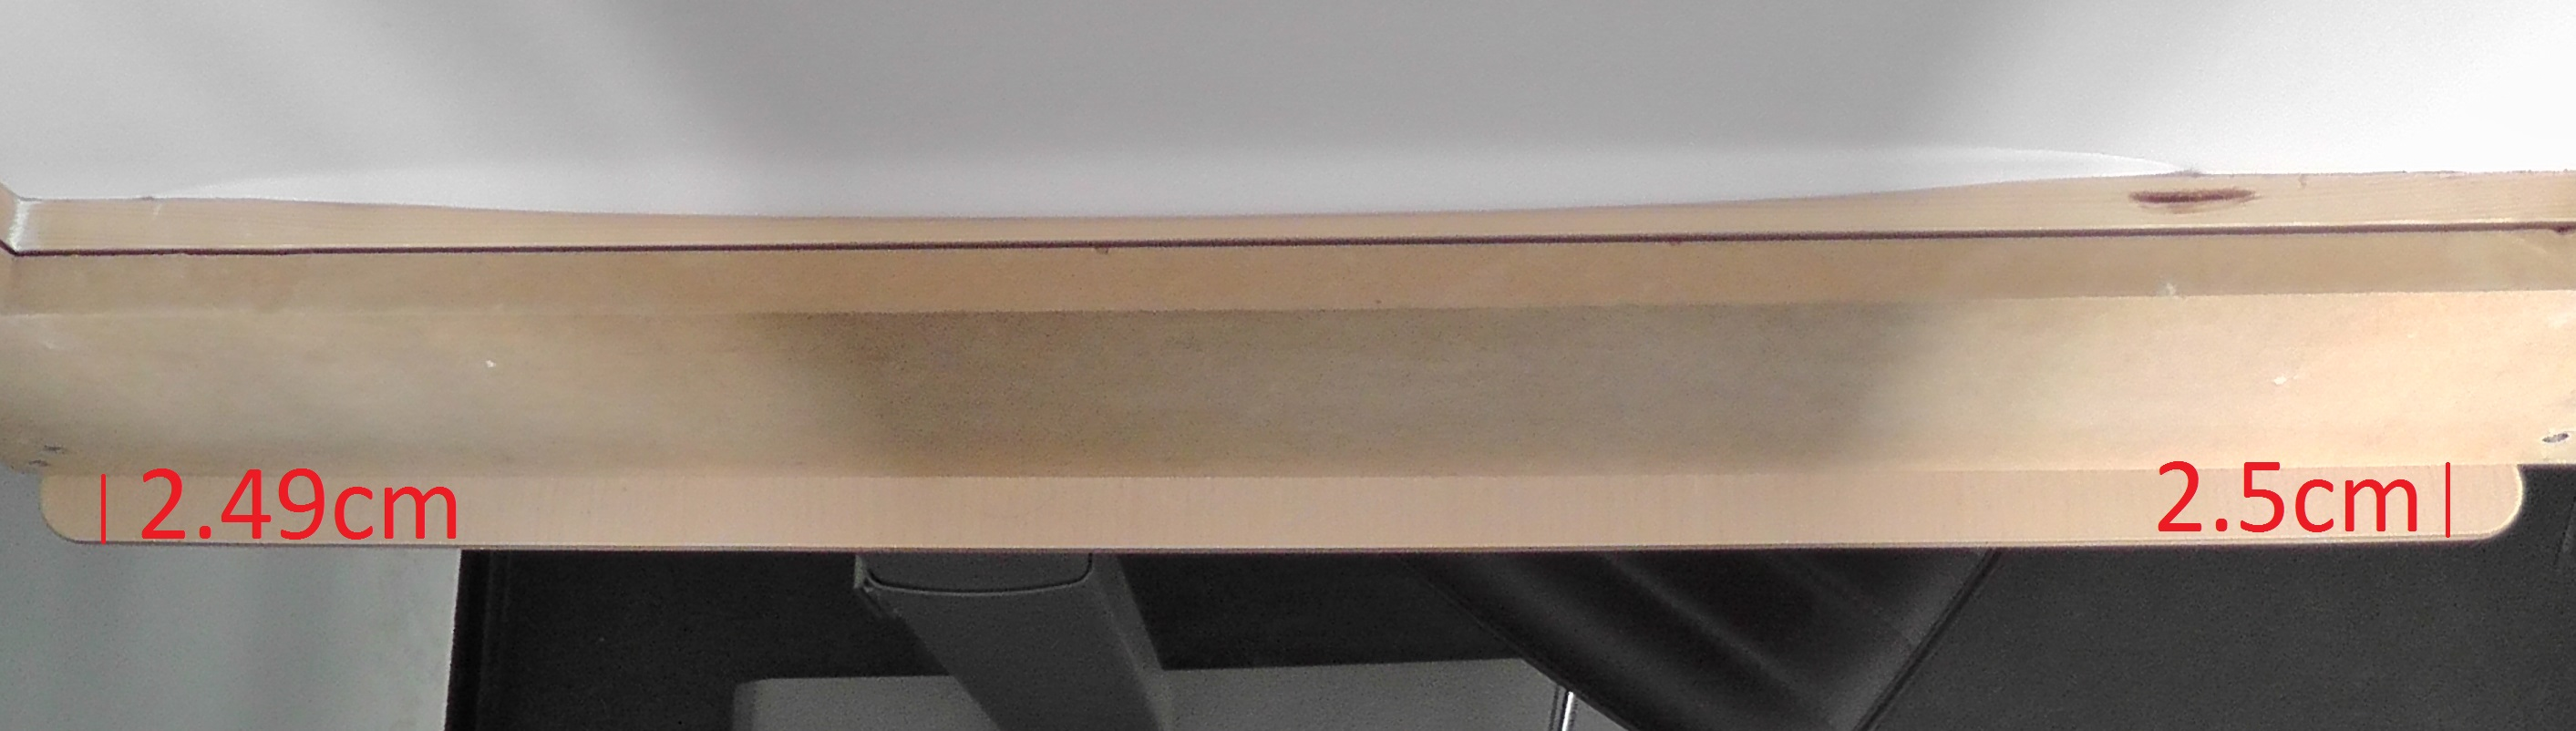
\includegraphics[width=0.85\textwidth]{figures/FramePlacementCM.jpg}
     \caption{The frame placement. Distance is displayed in red.}
     \label{fig:FramePlacement}
 \end{figure}
 
An application that allows a user to manually specify a number of points in the image and subsequently returns the depth values corresponding to these points, has been developed(see figure \ref{fig:PointDepthExtraction}). It is using the OpenCV(see \cite{opencv}) and Intel Perceptual Computing libraries. The former was used for displaying the image, reacting to mouse input and drawing the crosses, while the latter provided the depth frame data from which the image was created. The depth has been returned in millimeters, and for the points in figure \ref{fig:PointDepthExtraction}, the values were: 689 for top left, 685 for bottom left, 701 for top right, 702 for bottom right. From these values, it appears that there is a small vertical offset(1-4 mm), and a larger offset on the horizontal axis(7-11 mm). The test was repeated several times, and the general pattern was the same - larger horizontal offset and smaller vertical offset. However, the obtained values shifted overall with up to 2-3 centimeters, between different frames and points. While the relative offset patterns were largely the same, there were a few exceptions, when the vertical offset was also large on one side. However, this issue, along with that of the points being shifted, may be caused due to noisy data, as the points in those cases were very near to the top or bottom edge of the valid depth data(where we can also see some small dark spots).
 
  \begin{figure}[hbtp]
      \centering
      \includegraphics[width=0.7\textwidth]{figures/PointExtractionDepthMP.PNG}
      \caption{Points for which depth had been extracted and compared.}
      \label{fig:PointDepthExtraction}
  \end{figure}


Note that if calibration is used, the offset introduced from incorrect orientation and positioning is applied to the virtual camera view. Therefore, as long as the projector would be physically aligned to the cloth and the cloth would be fully in view of the depth camera, the setup would work fine. It would not be necessary to have the camera aligned perfectly in the physical world.

\subsubsection{Virtual projector alignment to the cloth area}

The virtual “slide projector” displays a texture onto the mesh of the cloth display. When looking at the display's mesh in wireframe mode(see figure \ref{fig:TextureAlignmentToMeshArea}), we can distinguish what roughly represents the cloth area, because of depth variations with respect to the frame. 

\begin{figure}[!hbtp]
    \centering
    \includegraphics[width=0.85\textwidth]{figures/TextureAlignmentToMeshArea.png}
    \caption{Texture Aligned to Cloth Surface. The area inside the red rectangle shows an offset.}
    \label{fig:TextureAlignmentToMeshArea}
\end{figure}

Due to the fact that the cloth mesh is rotated, the texture can not be aligned perfectly(in order to do this, proper calibration is required; see figure \ref{fig:MisalignmentArea}). Otherwise, a texture with 4 red corners and a grid has been used to test if the grid looks fairly straight and the corners roughly correspond to the edges of the cloth. 

The offset is not easy to see in the previously mentioned figure, but an arrow points to the line which separates the wooden frame from the cloth. The line is a bit thicker and we can think of it like a delimiter. If you look closely, you can see that the line is steadily going upwards as it advances towards the right side. If the texture would have been aligned perfectly, that line would correspond to the top line of the grid.



\begin{figure}[!hbtp]
    \centering
    \includegraphics[width=1.0\textwidth]{figures/MisalignmentArea3.png}
    \caption{The area has been magnified. An arrow points towards the line that separates the frame from the cloth.}
    \label{fig:MisalignmentArea}
\end{figure}

In order to align the texture better, or at least, make the debugging process easier, we could calculate the normals for the mesh and show the shaded object. Further, we could also add color information(then we would have a full 3D model, which resembles the physical object, making it easier to see where the texture should be projected).

\subsubsection{Virtual camera alignment to the cloth area}
\label{sec:VirtualCameraAlignmentToClothArea}

The virtual camera was aligned by computing the projection and view matrices, by trial and error, so that it completely covers the previously aligned texture. The projection matrix was computed via the \verb|glm::perspective| method, which requires the vertical field of view, the aspect ratio and the near and far planes. The aspect ratio was set to $16:9$, and the near and far to $0.1$ and $1000$, respectively. The field of view(\verb|FOV|) was the parameter that was computed by trial and error. If we have the intrinsic parameters, the field of view can be obtained, or alternatively, we can obtain all of the frustum planes with these parameters(\textit{left}, \textit{right}, \textit{bottom}, \textit{top}; \textit{near} and \textit{far} can be specified manually). For the latter, \verb| glm::frustum| could have been used.

Next, for the view matrix, we simply use a modelview matrix, of the form described in figure \ref{fig:MVMatrix}. The matrix is set in the code by specifying every element manually. If we have the extrinsic calibration parameters, we need to use the translation parameters for the last column, and the rotation parameters for the first three columns in the matrix. The last row remains unmodified.

As mentioned, the camera was moved around the scene until it roughly had the texture in view. The field of view and distance of the camera have been adjusted to that effect, but, it is important to note that there is an infinity of ways to combine these two values in order to roughly have the texture in view. This is because, we can always increase the field of view, and decrease the z distance, or vice versa. Now, the important issue here, is that the image will not look the same for all different combinations of values! For example, if we move the camera closer to the mesh in the virtual world while decreasing the FOV, we will see more aliasing(noise), but the distortion compensation is also more pronounced. Conversely, if we move the camera further away while increasing the FOV, we will have a more stable image, but the distortion effect is less pronounced. In order to get accurate results, one needs to calibrate the system in order to obtain proper parameters. However, it is still possible to set the value to acceptable levels by trial and error.

The values were set manually as explained above, and the system was tested via comparisons of images and video sequences, representing the differences between distortion compensation and non-compensation, and an empirical study. If the results from these tests are positive, meaning that the compensation improves the quality of the image(to some degree), by making it look more like on a flat screen, then it is reasonable to assume that, if the setup is calibrated, the distortion correction will be of higher quality. However, another set of tests would be necessary in order to verify this. The empirical study is described in section \ref{sec:EmpiricalStudy}.

\subsubsection{Testing precision of alignments}

Finally, in order to test how well the system is aligned, tests were made with single finger interactions, where the pushed finger corresponds to the maximum slope(minimum depth distance from the camera). A color coding scheme has been used for testing. First, just by using a red color for testing the finger's tip, and then several colors, to distinguish a larger area around the interaction point. 

The results were accurate in the center, as you can see from the figure \ref{fig:CenterPointCalibration}. The area surrounding the finger was drawn roughly in the center, in both images(the size of the area was determined by a threshold). In \ref{fig:RedCenterDotPhysical} we can also see that after pushing into the display, the red dot still appears around the finger.

\begin{figure}[!hbtp]
\centering
\begin{subfigure}{.5\textwidth}
  \centering
  \includegraphics[width=0.9\linewidth]{figures/RedCenterDotPhysical.JPG}
  \caption{Pushed area on cloth, shown red.}
  \label{fig:RedCenterDotPhysical}
\end{subfigure}%
\begin{subfigure}{.5\textwidth}
  \centering
  \includegraphics[width=0.9\linewidth]{figures/RedCenterDot.JPG}
  \caption{Pushed area on screen, shown red.}
  \label{fig:RedCenterDot}
\end{subfigure}
\caption{Correspondence between physical and virtual images.}
\label{fig:CenterPointCalibration}
\end{figure}

However, when testing towards the sides, the results were worse, and the offset grew larger. This is probably due to the fact that the surface is rotated. The results are shown in figure \ref{fig:RightPointCalibration}, with the detected area being very small. However, we can still see that the image shifts when seen on the cloth, and the red area is no longer aligned with the finger. Considering this, it is much more likely that the image will be correctly shifted(undistorted) only in the center area. Some further testing and adjustments could perhaps reduce the offsets and increase the quality of the distortion correction.

Please do no try to look for the distortion compensation effect in these figures, because they have been captured at an angle and you will not see the correct effect. For the compensation please take a look at  the video(see appendix \ref{appendix:A}) or section \ref{sec:comparison}, where the results are also discussed.

\begin{figure}[!hbtp]
\centering
\begin{subfigure}{.5\textwidth}
  \centering
  \includegraphics[width=0.9\linewidth]{figures/RedRightDotPhysical.JPG}
  \caption{Pushed area on right side of cloth, shown red.}
  \label{fig:RedRightDotPhysical.JPG}
\end{subfigure}%
\begin{subfigure}{.5\textwidth}
  \centering
  \includegraphics[width=0.9\linewidth]{figures/RedRightDot.JPG}
  \caption{Pushed area on right side (screen view), shown red.}
  \label{fig:RedRightDot.JPG}
\end{subfigure}
\caption{Correspondence between physical and virtual images.}
\label{fig:RightPointCalibration}
\end{figure}

%\newpage
\clearpage
\section{Empirical Study Design}
\label{sec:EmpiricalStudy}

A user study was done in order to find out how the distortion compensation is perceived by end-users(to test how well it works), if the behavior is consistent in different areas of the display and whether users prefer this solution to an uncompensated image. 

\subsection{Methods}

Each user was presented two methods of displaying the image onto the cloth: A and B. One of these methods represented the distortion compensation method that is the focus of this report, while the other was just a regular image, projected onto the cloth. 

\subsection{Hypotheses}
\label{sec:hypotheses}
In order to learn whether the developed method compensates the image and corrects the distortion, whether it is reliable, preferred over an uncompensated image, or whether it is actually distinguishable from a normal projection, the following hypotheses were considered:

\begin{itemize}
\item Difference between the two methods\\

It is expected that the compensation will change the image in a significant way, thus allowing participants to easily see a difference between the methods
\item Preservation of Appearance\\

Although the compensation is not perfect, it is expected that the compensated method is superior when it comes to preserving appearance(original image proportions), relative sizes, etc.
\item Consistency\\

Since the system has not been properly calibrated, I do not expect the compensation to perform in a consistent way in all areas of the display. The uncompensated method is expected to be more consistent(since the image is not compensated).
\item Preference\\

Since distortion correction helps interaction, by keeping objects in the same positions and shape, even if the display is deformed, it is expected that the compensated method will be preferred(even if it does not work perfectly).
\end{itemize}


\subsection{Apparatus}

Participants had to switch between methods A and B, by using a mouse as an input device. As seen in figure \ref{fig:Mouse}, the mouse had two labels, denoting which button must be pressed to select a particular method. Moreover, it was attached to the display's frame, which made it easy for users to interact with it. This input method allowed the users to compare the visuals while interacting with the display, and at their own pace. Further, this enabled the use of the same images in both methods A and B, without providing visual cues on the actual textures(since they could easily switch between them to see which is the active method).  In certain cases, when two-hand interactions were required, I switched between the two methods for the users. Moreover, the tasks were also changed by me. 

\begin{figure}[!hbtp]
    \centering
    \includegraphics[width=0.6\textwidth]{figures/UserStudyMouseInput.JPG}
    \caption{The input device for switching between the methods.}
    \label{fig:Mouse}
\end{figure}

\subsection{Participants}

Two pilot studies were conducted in order to find and fix any critical flaws in the design of the study. A total of 11 participants tested the system on the deformable cloth display in the final version of the study. The participants were all students, aged between 23 and 31(with a mean of 25.9) years old. 2 participants were female and 9 were male. Further, the participants were standing during the study, so they were also asked for their height, which varied from 1.65m to 1.87m(with a mean of 1.74m). Some adjustments had to be made for the shortest and tallest, but these did not prove to be a problem. Moreover, one of the participants described that he had a vision problem on the right eye, however this did not seem to affect his experience during the tasks.

Further more, each participant was informed that the duration of the study is expected to be around 45 minutes(the longest actual session was probably close to an hour). Participants were compensated with a bottle of wine or box of chocolates, at the end of the session.

3 of the participants had prior knowledge about the display, but only one of them had experience in using it. The actual scenarios and methods were unknown to all participants.

\subsection{Design}

The participants were asked to compare the two methods, regarding the preservation of appearance(proportions similar to the original image, projected onto a 2D surface), or whether they see a difference at all. Further, 5 scenarios were designed, and the users had to test both methods in all scenarios. The motivation behind these scenarios as well as a description of each is discussed in section \ref{sec:scenarios}.

Next, methods A and B were also given in a random fashion - so that they are counterbalanced.  Moreover, the scenarios have also been shown to the participants in a different order, so that the data is not biased for a particular scenario configuration. Therefore, each scenario was assigned a number between 1 and 5, and a latin square was used in order to decide the scenario configuration for the following experiments. Each row from the square(the same scenario configuration) was used once for each combination of A and B(once when A was the compensating method, and once for B).

In the following sections, each scenario will briefly be described in addition to the other documents used in the study, including the questionnaire.

\subsection{Scenarios}
\label{sec:scenarios}

Several scenarios were developed in order to test the compensation for different situations - this was done in order to find out, if the compensation behaves in similar ways and whether it is preferred by users, in different contexts. Further, another reason for this is multiple testing  - this is required in order to give users some time and variety, so that they can reach a decision on what method preserved the image proportions better, was preferred, etc. It can be noted that some users changed their minds after one scenario, because they hadn't notice something before. In situations like these it is helpful to have multiple tests. The scenarios and the motivation for each one of them will be described in the following sections.

\subsubsection{Grid, Text and Columns Scenarios}

 The \textit{Grid Scenario} was chosen because it is easier to see if the vertical and horizontal lines remain relatively straight after deformation, compared to a detailed scene. Further, it is also interesting to see if text can retain it's shape after deformation, allowing the user to still read the words in the deformed area - for this reason, the \textit{Text Scenario} was used. Finally, the \textit{Columns Scenario} consists of a few objects of interest, namely columns. When one deforms the display, these columns bend, meaning that a compensated image should make them look straight. Further more, the display can also be deformed in the middle, between the columns, that also causes bending if the image is not compensated. Since the columns are placed on the sides, it is a good way to test the same objects, by interacting in different areas of the screen. In addition, the scene is 3D, so unlike the other scenarios, we can check if the depth between the objects is corrected.

 Due to these three scenarios being very similar, they will all be explained in one section. They all consisted of displaying a static image: of a grid, some text, and a number of columns in a scene, respectively. For each of these scenarios the users had to share their thoughts on methods A and B, for three different points in the image(see figure \ref{fig:GridTextColumns}). For these scenarios, they only used one finger interactions to deform the display at the indicated points(by using the index finger). Only one point was shown at a time, and it was made invisible after the participant remembered where the point was positioned.


\begin{figure}[!hbtp]
\centering
\begin{subfigure}{.33\textwidth}
  \centering
  \includegraphics[width=0.9\linewidth, height=3cm]{figures/grid_hd_allPoints.jpg}
  \caption{Grid scenario.}
  \label{fig:GridTexture}
\end{subfigure}%
\begin{subfigure}{.33\textwidth}
  \centering
  \includegraphics[width=0.9\linewidth, height=3cm]{figures/random-text-2048x2048_complete.jpg}
  \caption{Text scenario.}
  \label{fig:TextTexture}
\end{subfigure}
\begin{subfigure}{.33\textwidth}
  \centering
  \includegraphics[width=0.9\linewidth, height=3cm]{figures/3D_Scene_011_allPoints.jpg}
  \caption{Columns scenario.}
  \label{fig:ColumnsTexture}
\end{subfigure}
\caption{Grid, Text and Column Textures. Red dots indicate interaction areas.}
\label{fig:GridTextColumns}
\end{figure}

As you can see, the dots are not in the same positions, except for the center. This probably affects the results to some extent, since the compensation seems worse as one advances towards the sides of the image. However, the points were placed with the texture contents in mind - for example, having the red circles on the columns, or on a particular word, for the respective scenarios. The three points were coded: \textit{left}, \textit{center} and \textit{right}(with left meaning left-most and similarly for right). Even though the left and right points are not in the same positions, the same patterns were observed for all three scenarios, as presented in section \ref{sec:Results}.

Finally, for each scenario, users were told to look at some particular aspect of the current image, in order to give their opinion on how distorted the image is, when compared to how it would look on a flat display:
\begin{itemize}
\item For the grid, users were asked how straight the black lines appear with each method
\item For the text, users were asked to look at the space between the lines, readibility, and how similar the word appears to one on a flat screen
\item For the columns, users were asked to look at how straight the columns appear after pushing into the display
\end{itemize}

\subsubsection{Map Scenario}

Map navigation is another useful task and it could be used in some interesting ways on deformable displays such as zooming in on a particular area of interest. However, the test is only concerned whether the compensation makes the image look more like the original map.  This is required because, if one were, for example, to push in and select a landmark on the map, the area would be hardly visible without compensation, since the cloth in that area would approach the projector, making everything much smaller. In addition, the area would also be curved, making it even harder to see the deformed zone.

The map scenario simply consisted of a static map texture of a region of \textit{New York City City}(see figure \ref{fig:Map}). Users were asked to push into the display, using two hands. Further, they were also instructed to focus on the central area of the display. Then, the users were asked to compare the proportions and readability of the image, with both methods. Further, users were also instructed to focus on some particular name or landmark to focus on, as this makes it easier to compare.


\begin{figure}[!hbtp]
    \centering
    \includegraphics[width=1.0\textwidth]{figures/NYMidZoomA.jpg}
    \caption{A map showing a region of New York City. Courtesy of Google Maps.}
    \label{fig:Map}
\end{figure}

\subsubsection{CT Brain Scan Scenario}

Since we are using a deformable display, one of the visualizations that makes sense to test is that of 3D volumes, represented using \textit{slices}(textures). This is because these slices are changed based on depth and we can simulate this by pushing an pulling into the display. Further, volume slicing interaction means we can also test how the compensation works when we have a dynamic scene/object. However, an issue with this scenario was that the slices were changing too fast, which in turn changed the shape of the object(brain) and made it more difficult for users to judge the compensation effect.

This scenario consists of a number of textures, representing volume data for a brain scan. The texture set was taken from the \textit{Stanford volume data archive}(available at \cite{levoy2001}). Users had to use two-hand push gestures in order to advance, or two-hand pull gestures to reverse, through the \textit{slices}(textures). The starting texture was in the middle of the dataset. Again, the objective was to compare methods A and B. Since the brain is changing shape throughout the slices and the the speed is too fast, it can be hard to see the differences. Several users complained about this, and, if they could not see a difference, they were instructed to compare the methods for the last image(see figure \ref{fig:BrainSlices}), using the push gesture.


\begin{figure}[!hbtp]
\centering
\begin{subfigure}{.5\textwidth}
  \centering
  \includegraphics[width=0.9\linewidth]{figures/brain_043.jpg}
  \caption{Starting scenario volume slice.}
  \label{fig:StartBrainSlice}
\end{subfigure}%
\begin{subfigure}{.5\textwidth}
  \centering
  \includegraphics[width=0.9\linewidth]{figures/brain_098.jpg}
  \caption{Last volume slice.}
  \label{fig:EndBrainSlice}
\end{subfigure}
\caption{CT scan of a brain. Example of two different textures(slices). Courtesy of \cite{levoy2001}}
\label{fig:BrainSlices}
\end{figure}

For details on how the interactions in this scenario were implemented(so that the slices update), please see appendix \ref{appendix:B-vsi}.

\subsection{Procedure}

Before starting the experiment, each user was given a short text to read, which presented basic information on the experiment in which they were about to partake. Next, they were introduced to the cloth display and the distortion problem was explained and shown to them. Further, they practiced the gestures that they were about to use during the experiment: one finger gesture and two-hand push and pull gestures. 

Following this introduction, the participants were then asked to go through all of the scenarios, while comparing methods A and B. In addition, (a part of) a  questionnaire was given to the users after each scenario. If the questionnaire would have been only given at the end, it would have been hard for the users to remember the details about each method, for all scenarios. This fact was also uncovered during one of the pilot sessions.

Finally, I was sitting at a desk behind the users, so I could watch the participants go through the tasks, while also keeping notes. I also asked interview questions, while they were interacting.  

\subsection{Reducing Visual Differences Between Methods So That They Are Not Easily Recognizable}

Two pilot tests were performed, before the actual user study. From these, an important issue surfaced. Users could easily spot which method is the normal one, because there was no noise in the image, while the distortion correction methods introduced aliasing-like effects, other noise and black areas, due to invalid depth data(while interacting). 

One attempt to solve the problem was to use depth smoothing as described in section \ref{sec:DepthSmoothing}. The final result after spatial and temporal averaging was still not good enough - you could still see the difference between the two methods, because of the dynamic noise in the compensated image. However, the smoothing did reduce the overall noise and improved image quality. 

Since noise reduction did not solve the issue, the remaining options were to either introduce noise in the other image, by some function or random pattern, or, the solution which was actually employed, capturing a number of frames rendered with the distortion correction method and displaying them continuously as the normal method. This approach made the images look very much alike when the display was not deformed. Consequently, this served as a good way to avoid any bias coming from comparing a normal image with a noisy one. Most users did not realize that the other method was just a normal image(or actually 10 frames which keep repeating). Even some users, who had the impression that the normal method does not help at all with correcting the distortion, assumed that the method is doing something, because of the dynamic noise in the image.

\subsection{The Questionnaire}

The questionnaire is composed of several parts. On the first page, the participants were given some basic information about the structure of the questionnaire and they were also asked for demographic data. This page was given to the users after completion of the first scenario, with an additional page with the questions for that particular scenario - questions for each scenario were given on a separate page. Finally, there were some common question in the end, which asked the participant to rate method A and B overall. Although the main aspects of the questionnaire will be described below, the document can be consulted in appendix \ref{appendix:C}.\\

The questions mainly related to the attributes described in relation to the hypotheses(see section \ref{sec:hypotheses}).
\begin{itemize}
\item Perceived difference between the two methods \\{[Not Different - Very Different]}
\item Preservation of appearance(proportions) for each method \\{[Very Poor - Very Good]}
\item Method preference [A - B]
\end{itemize}
Feedback about these was collected to gain some insights on whether end-users perceive differences between compensation and non-compensation, whether the compensated method preserves the original image proportions better and whether one of the methods is preferred.

The preservation of appearance is related to the resemblance to the original image, as it would appear on a flat display(how similar are the relative proportions, with respect to the original image?). Next, the subjective preference is asked for, because it is possible that a user does not like a method, even if it works correctly - qualitative feedback has been obtained in order to determine if this is the case. Lastly, the attribute that is being rated is shown in brackets in the section above(the ends of the scale).

To be more concrete, the questionnaire contained the following items:
\begin{itemize}
\item Difference between the two methods
\item Please explain in what way were the methods different
\item Preservation of appearance during deformation - Method A
\item Preservation of appearance during deformation - Method B
\item Method preference for this scenario
\item Please explain why you have preferred the selected method
\end{itemize}

In addition, the grid, text and columns scenarios had two additional questions, regarding how consistent the behavior was, in the different areas of the display - for the three tested points(e.g.: a method could work very well in the center, but have poor results on the sides):
\begin{itemize}
\item Method A's behavior was consistent, for all points \\{[Not Consistent - Consistent]}
\item Method B's behavior was consistent, for all points \\{[Not Consistent - Consistent]}
\end{itemize}

An 11-point scale has been made available for users to rate all the attributes. The scale starts at 0 and ends at 10; it has been originally adapted from the QUIS 10-point scale(examples at \cite{quis}). An 11-point scale was used instead, so that the user also has a neutral option – otherwise they would have been forced to “prefer” one of the methods. As mentioned before, the questionnaire also had more descriptive items, where participants were asked to motivate their choice of their previous rating.

\subsection{Questions During the Tasks}

Some questions were also asked during the tasks. The questions are in the \textit{scenario notes} document, available under appendix \ref{appendix:C}. For the scenarios with the grid, text and columns feedback was collected regarding all of the three points tested. Similar scenario-specific questions were asked, as mentioned in the document(e.g.: how straight do you think the grid lines appeared with method B?).

For all scenarios, the participants were generally asked to describe the methods using their own words. Moreover, they were reminded to look straight at the area they are deforming. Further more, they were also asked whether the noise in the image affects the tests in any way.

\newpage
\section{Analysis of Results}
\label{sec:Results}
\subsection{Empirical Study Results}
\label{sec:Empirical Study Results}
 As described in chapter \ref{sec:EmpiricalStudy}, each participant tested both the compensated method, and a normal image projection. The two methods have been alternated between participants - the first had method A as the compensated and B as the normal image, while the second had A as the normal and B as the compensated, etc. Further, the experiment consisted of 5 scenarios, which have also been shown to the participants in a different order, so as not to bias the data for a particular scenario configuration. Finally, smoothing functions were applied on the compensated method in order to reduce noise. However, this was not enough, as dynamic noise could still be seen in the image. Therefore, noise was added to the normal method, by capturing 10 frames of the compensated method and replaying them in a loop. This meant that the users could not easily identify the method due to visual artifacts, because they were present in both methods.

Three of the participants had seen the display before the experiment. However, a strong bias due to the previous reason is unlikely, since they had not seen the actual experiments/scenarios before.

Since feedback is of both quantitative and qualitative nature(questionnaire + interview questions), both were used in order to draw conclusions on the outcome of the experiment.

In order to analyze the quantitative results, paired t-tests have been run for both the consistency and preservation of appearance questions. These tests help to determine the statistical significance of that particular comparison.

Further more, t-tests have also been run on the preference as well as on the overall preservation of appearance questions. However, it is very important to note that there was only one question related to the previous items, where the user had to compare between methods A and B on an 11-point scale from 0 to 10. In order to get some meaningful results, the scale has been converted, so that both the compensated and the non-compensated method could be rated from 0 to 5(e.g. 0 represents 5 for method A, while 10 represents 5 for method B, and 5 represents 0). The values were separated into compensated/not\_compensated categories and the missing values were replaced with 0. Differences are shown in table \ref{table:DifferenceTable}.

The qualitative data has been grouped in a few categories(e.g.: distorted, preserves appearance). Only the qualitative data regarding the center, left and right points for the grid, text and columns scenarios and the qualitative data in the overall case, have been analyzed. Most of the qualitative feedback for the three previously mentioned scenarios could be grouped by the three points. It may have been confusing to look at how the scenario was said to behave over all of the points, since in many cases the results differed quite a lot between them(for example, a user could have stated that method A for scenario 1 was distorted twice, and not distorted once; however, feedback such as - "it was not distorted in the center, but distorted to the left or right" is much more useful).

In the following, the full analysis will be described. We start by looking at perceived difference between the methods, then proceed to look at preservation of appearance, consistency and finally, preference. Please note that the aggregated data(e.g.: mean and standard deviation) for all pairs of scenarios is only shown in appendix \ref{appendix:B-agg}. The values were computed from the raw data with both a spreadsheet and IBM SPSS(details at \cite{spss}).

\subsubsection{Quantitative Analysis}
\paragraph{Difference}\mbox{}\\

One of the items on the questionnaire asked users whether they can see a difference between the compensated and non-compensated methods. The means of the results are shown in table \ref{table:DifferenceTable}, for each scenario. We can see that the map scenario had the highest perceived differences(although it seems that the grid comes close, and has a lower standard deviation), while the brain scan scenario had the lowest. For the latter, a problem was that the shape was changing too fast as the user was interacting, which made it hard to make out differences. However, in order to solve this issue, the user was then told to only compare the methods for the last slice in the set, which remained static.

%\begin{figure}[!h]
%    \centering
%    \includegraphics[width=0.85\textwidth]{figures/results/DifferenceChart.PNG}
%    \caption{Mean of perceived differences between methods, per scenario.}
%    \label{fig:DifferenceChart}
%\end{figure}

\begin{table}
\begin{center}
    \begin{tabular}{ | l | l | l |}
    \hline
    Scenario & Mean & SD \\ \hline
    Grid & 7 & 1.67 \\ \hline
    Text & 6 & 1.84 \\ \hline
    Columns & 6.54 & 1.63 \\ \hline
    Map & 7.36 & 2.01 \\ \hline
    Brain Scan & 4.18 &  2.48 \\
    \hline
    \end{tabular}    
    
\end{center}
\caption{Perceived difference between the two methods, for all scenarios.}
\label{table:DifferenceTable}
\end{table}


The mean values are approximately in the [4.18, 7.36] interval, from a rating on an 11-point scale from 0 to 10. This shows that at least moderate differences were observed between the two methods, for all scenarios.

\paragraph{Preservation of Appearance}\mbox{}\\

There are a total of 5 pairs that have been tested for significance using a paired t-test. Each pair corresponds to one scenario. The actual results are shown via a bar chart in figure \ref{fig:POA_Graph}. All scenarios have the mean shown for both compensated and normal methods. We can also see visually, that the highest differences are in the Map Scenario, with the compensated method being rated much higher. Further more, we can also see that the compensated method scored higher, for all scenarios which indicates that it preserved appearance better.

\begin{figure}[!h]
    \centering
    \includegraphics[width=1.0\textwidth]{figures/results/POA_Graph.PNG}
    \caption{Mean of preservation of appearance, per scenario.}
    \label{fig:POA_Graph}
\end{figure}

In addition, the vertical error bars show the standard error, and it can be used as another measure for statistical significance by checking if the bars from the two different methods overlap(see \cite{error_bars} for more details on this procedure). We can see that the only scenario for which there is no overlap is Map. Although this does not tell us if the results are statistically significant, it does tell us that all the other cases are not(when there is an overlap, we can be sure that the results are insignificant).

However, it is useful to also look in a bit more detail at statistical significance. The output of the t-tests is shown in table \ref{table:POA_Test}. Note that a \verb|*| symbol has been used to denote statistical significance. For all other cases, the null hypothesis could not be rejected. Since the confidence interval is 95\%, we would normally need a significance level of $<= 0.05$. However, we have a case of multiple testing, because we have one hypothesis tested for each scenario. As described in \cite{bonferroni}, we need to adjust the parameter $\alpha$, by dividing it with the number of tests(Bonferroni correction). In this case we have $\alpha = 0.05$ and $n$ = 5, which gives $\frac{\alpha}{n} = \frac{0.05}{5} = 0.01$. We must test against this value rather than the original $0.05$. However, in this case, the results are not affected.


%\begin{table}[!h]
%  \includegraphics[width=\linewidth]{figures/results/POA_Test.PNG}
%  \caption{T-test results for preservation of appearance. The * indicates statistical significance.}
%  \label{tabel:POA_Test}
%\end{table}

\begin{table}
\begin{center}
    \begin{tabular}{ | l | l |}
    \hline
    \textbf{Pair(C \& NC)} & \textbf{p-value }\\ \hline
    Grid & .157 \\ \hline
    Text & .341 \\ \hline
    Columns & .472 \\ \hline
    Map & \textbf{.000*} \\ \hline
    Brain Scan & \textbf{.097} \\
    \hline
    \end{tabular}    
    
\end{center}
\caption{T-test results for preservation of appearance. The * indicates statistical significance. C denotes compensation method and NC the non-compensated.}
\label{table:POA_Test}
\end{table}

To conclude this part, both the table and the chart indicate that the only statistically significant scenario is Map. The table tells us that the result is actually significant, while the chart can also be used to rule out the other cases, as well as providing a helpful visual indicator of the degree of difference for the two methods, for preservation of appearance. Moreover, it is possible that we have a trend for the Brain Scan scenario since the pair's value is  value is $< 0.1$, but all other cases are insignificant(a larger user pool may improve results).

\paragraph{Overall Preservation of Appearance}\mbox{}\\

A separate question was asked for overall preservation of appearance. This case has not been included previously because the results are on a different scale. All other questions about preservation of appearance were asked twice, once for each method. However, there is only one question for the overall case, which asked the participants to rate the preservation of appearance on an 11-point scale from 0 to 10, where 0 denoted the maximum preference for method A, while 10, for B, with 0 as a neutral option. The results were mapped to [0,5] as mentioned previously, at the beginning of this section. 

The graph in figure \ref{fig:OPOA_Graph} shows the contrast for the results between the two methods. We can see that the preference was clearly for the compensated method, though the degree of preference is maxed somewhere between 2 and 3, out of a maxim of 5, which suggests that, even though the method did help to correct the image so that it appears as on a flat display, there still is room for improvement. Removing some of the visual artifacts, as well as calibrating the system to ensure that the compensation is of high quality, should improve the degree to which participants prefer the compensated method. Moreover, the standard error bars do not overlap, which indicates that the test may be statistically significant. 

\begin{figure}[!h]
    \centering
    \includegraphics[width=0.85\textwidth]{figures/results/OPOA_Graph.PNG}
    \caption{Mean of preservation of appearance, overall.}
    \label{fig:OPOA_Graph}
\end{figure}

Moreover, the t-test results are shown in table \ref{table:OPOA_Test}; note that this time we only have one pair. As mentioned before, the missing values were replaced with 0 when running the t-test(the user was forced to select a preference for either method A or B). The results are statistically significant, with a value comfortably below the $0.05$ threshold(there is no need for a correction in this case, since the question is not asked for each scenario, so we only have one test). 

%\begin{table}[!h]
%  \includegraphics[width=\linewidth]{figures/results/OPOA_Test.PNG}
%  \caption{T-test results for overall preservation of appearance. The * indicates statistical significance.}
%  \label{tabel:OPOA_Test}
%\end{table}


\begin{table}
\begin{center}
    \begin{tabular}{ | l | l |}
    \hline
    Pair(C \& NC) & \textbf{p-value }\\ \hline
    Overall & \textbf{.001*} \\
    \hline
   	\end{tabular}    
    
\end{center}
\caption{T-test results for overall preservation of appearance. The * indicates statistical significance}
\label{table:OPOA_Test}
\end{table}

In conjunction with the error bars from the graph, we can conclude that there is a substantial, statistically significant preference for the compensated method, albeit with a relatively modest degree of preservation. Moreover, only one participant preferred the method which had not been compensated, so there is an almost universal preference for the compensated method, regarding overall preservation of appearance.

%\begin{figure}[!h]
%    \centering
%    \includegraphics[width=1.0\textwidth]{figures/results/OPOA_Area.PNG}
%    \caption{An area chart showing the perceived overall preservation of appearance, for both methods and all participants.}
%    \label{fig:OPOA_Area}
%\end{figure}

\paragraph{Consistency}\mbox{}\\

The consistency refers to the behavior of the methods in different areas of the display, and it has only been tested for three scenarios: Grid, Text and Columns, where the participants had to interact with three different points placed towards the center, left and right side of the screen.The graph in figure \ref{fig:Consistency_Graph} shows the results visually. We can see that we got similar values for all scenarios, with the uncompensated method always scoring higher. However, the standard error bars overlap for all cases, which indicates inconclusive results.

\begin{figure}[!h]
    \centering
    \includegraphics[width=0.85\textwidth]{figures/results/Consistency_Graph.PNG}
    \caption{Consistency mean, per scenario.}
    \label{fig:Consistency_Graph}
\end{figure}

Next, the t-test results are shown in table \ref{table:Consistency_Test}. Note that the consistency tests between methods is statistically insignificant for all scenarios.

%\begin{table}[!h]
%  \includegraphics[width=\linewidth]{figures/results/Consistency_Test.PNG}
%  \caption{T-test results for consistency. None of the tests were statistically significant.}
%  \label{tabel:Consistency_Test}
%\end{table}

\begin{table}
\begin{center}
    \begin{tabular}{ | l | l |}
    \hline
    \textbf{Pair(C \& NC)} & \textbf{p-value }\\ \hline
    Grid & .221 \\ \hline
    Text & .264 \\ \hline
    Columns & .398 \\ 
    \hline
    \end{tabular}      
\end{center}
\caption{T-test results for consistency. The * indicates statistical significance. C denotes compensation method and NC the non-compensated.}
\label{table:Consistency_Test}
\end{table}

From the previous analysis it seems that the quantitative consistency tests did not provide significant results, since, when computing the Bonferonni correction, the significance level is: $\frac{\alpha}{n} = \frac{0.05}{3} = 0.016$, which is much less than any of the values obtained in the tests. However, qualitative information may provide more information on consistency, and whether there really was a perceived difference between the three interaction points, as the previously mentioned figure seems to indicate. We shall look at this aspect in one of the subsequent sections.
\\
\paragraph{Preference}\mbox{}\\

The graph in figure \ref{fig:Preference_Graph} shows all the preference ratings, color coded by method and clustered on scenarios. From the standard error bars, we see that only the Map and Overall cases may be statistically significant(similar to preservation of appearance), since the bars do not overlap for these cases.

\begin{figure}[!h]
    \centering
    \includegraphics[width=0.85\textwidth]{figures/results/Preference_Graph.PNG}
    \caption{Means of method preferences, per scenario and overall.}
    \label{fig:Preference_Graph}
\end{figure}

Moreover, we can also see the rather large preference for the compensated method, both for the Map and the Overall cases - with only 2 participants preferring the normal method(one participant rated  preservation of appearance as worse, when compared to the compensated method), while the other 9 preferring the compensation. This analysis indicates that, for the previous two cases, the compensated method has been preferred to a far greater extent than the other one, and the results are statistically significant.  

Similarly to the previous cases, the results of the t-tests are shown in table \ref{table:Preference_Test}. We can see that in this case we have 5 pairs, 1 for each scenario, and an additional one for the overall case. This is because there was only one combined preference question, where the user had to rate between method A and B on an 11-point scale, with 0 representing strong preference for A and 10 for B. We observe that we again have the map scenario and the overall case as significant(the chosen statistical level was $0.01$ after Bonferroni correction and $0.05$ for the overall case).

\begin{table}
\begin{center}
    \begin{tabular}{ | l | l |}
    \hline
    \textbf{Pair(C \& NC)} & \textbf{p-value }\\ \hline
    Grid & .181 \\ \hline
    Text & .711 \\ \hline
    Columns & .451 \\ \hline
    Map & \textbf{.002*} \\ \hline
    Brain Scan & .206 \\ \hline
    Overall & \textbf{.019*} \\
    \hline
    \end{tabular}    
    
\end{center}
\caption{T-test results for preservation of appearance. The * indicates statistical significance. C denotes compensation method and NC the non-compensated.}
\label{table:Preference_Test}
\end{table}
%\begin{table}[!h]
%  \includegraphics[width=\linewidth]{figures/results/Preference_Test.PNG}
%  \caption{T-test results for method preference. The * indicates statistical significance.}
%   \label{tabel:Preference_Test}
%\end{table}

%\begin{figure}[!h]
%    \centering
%    \includegraphics[width=1.0\textwidth]{figures/results/Preference_Area.PNG}
%    \caption{An area chart showing the perceived overall method preference.}
%    \label{fig:Preference_Area}
%\end{figure}

\subsubsection{Qualitative Analysis}
\label{sec:QualitativeAnalysis}
Qualitative data has been retrieved with two methods: 
\begin{itemize}[noitemsep,topsep=0pt]
\item Descriptive questions about all of the previous attributes: consistency, difference, preference, preservation of appearance.
\item Interview-like questions asked while the user was interacting. Some scenario specific questions were introduced, in order to make the user think how well the image is preserved.
\end{itemize} 

A substantial amount of data has been collected for each scenario. However, due to the nature of this experiment, participants described their experience using different words, even when faced with very similar questions. This makes it difficult to obtain meaningful measures for each scenario. Further, in some cases, for example, when the participants were stating that something is distorted, they repeated the test for each point(for the scenarios with three interaction points), which means that just knowing how many participants stated that a method is distorted is not as relevant as also knowing for which point the image was distorted. For example, the center point could have worked very well, but maybe, due to a high number of distortions on one of the sides, the overall scenario would have been ranked as distorted. Therefore, we start by analyzing the distortions around the interaction points from the interview. Naturally, this is only applicable to the three scenarios which consisted of a task for each point(shown as a red circles in the scenarios). Moreover, I grouped the feedback in a few categories: \textit{preserves appearance}, whether the image is \textit{distorted} or \textit{follows the finger}. This last category refers to the user's finger being in the same place after deforming the display, which would normally happen if the image correctly compensates for the distortion.

Note that I had some technical difficulties with one participant, where the uncompensated image appeared without the dynamic noise induced by the frames. In this test, the participant replied that the uncompensated method was more \textit{stable} and therefore preferred it. This issue became apparent when I asked whether the image quality affected their choice. This test configuration was repeated once again, with the last participant.

Before we delve into the previously mentioned aspects, it is important to mention that an issue with latency has surfaced - this will be described in the following section. 

\paragraph{Latency}\mbox{}\\

Although there was no specific question regarding latency, several users mentioned that the compensation has a "time delay" or that "it takes some time to adjust"(there are 5 such occurrences in total, mentioned by 3 different participants). During the study, the scenarios were run at about 30 fps, because it had the depth smoothing functions enabled. However, this issue was also mentioned by the participant in the second pilot study, when the frame rate was about 60 fps. Therefore, this issue may not be related directly to rendering, although this issue has not been investigated.
 

\paragraph{Center Point}\mbox{}\\


For this point, participants thought that the compensated method was preserving the appearance much  more often than the one which was not compensated(27 vs 3 occurrences). Some examples of items included in this category include: "keeps proportions better", "keeps the size of the object" for the uncompensated method and
"maintains proportions better", "better for the center", "resembles original better", "flattened image", "straighter". As we can see, the qualitative information is overwhelmingly in favor of the compensated method for this point. 

In addition, the non-compensated method also appeared distorted to users more often than the compensated one. Only two participants mentioned that the compensated method "distorts", versus 19 comments which mentioned that the uncompensated method was distorted: "deforms more", "does not do anything(follows shape of the cloth)", "distorting somehow".

Finally, the \textit{follow the finger} category was also in favor of the compensated method(more occurrences), but there were only a few results. From the 3 occurrences for the uncompensated method, two comments mentioned that "both follow the finger". This is because, in the center area of the display, it is more difficult to tell the difference, unless a more significant force is applied.

Clearly, the comments show that the compensated method was superior the other one(less distorted), in the center of the image.

\paragraph{Left Point}\mbox{}\\

For this point we have 12 occurrences of comments that mention the uncompensated method to preserve the appearance better: "straighter", "less distorted", "better because lines are straighter", "does not move", "looks more proportionate" etc., while only 8 comments to indicate that the compensated method preserves appearance:
"preserves better, but depends on push force", "feels more corrected on the point, but moves the image to the left", "adjusts the image more on the line", "keeps initial proportions". Although the uncompensated method was perceived to be better, we could find out that the image "moves to the left" and that the result depends on the applied force.

Regarding distortion, there were 19 comments for the compensated method ("distorts a lot", "deforming the image on the side", "the corner is more distorted", "it's going the wrong way - left, "letters go to the left", "moves to the left", "makes columns bend the other way") and only 6 for the uncompensated ("shifting everything", "doesn't compensate", "complete distortion", "perspective deformed"). From these comments we again see that the compensation is too much to the left of the deformed area, and actually, there are 8 such occurrences. This suggests this is the main problem, but one user also shared afterwards that "it was more corrected on the point", even though it looked very distorted. This happens because the setup is not calibrated, and the depth camera is not 100\% orthogonal to the display. This introduces misalignments near the sides if the camera is tilted, even slightly(which means the compensation will take place in a wrong area – with an offset; several users also complained of distortions “underneath the finger”).

Moreover, for this point there was an equal number of occurrences related to "following the finger"(3 for each method). For the uncompensated method, this phrase was mostly only used in conjunction with the word "better", but for the compensated, comments mentioned that it was "precise" and "closer to the finger". 

Even though the results were less accurate for this point, there still were 8 comments indicating preservation of appearance, while for the center point we only have 3 such occurrences for the uncompensated method. Therefore, if we take the results overall up to this point, it seems that they are still better for the compensated method.


\paragraph{Right Point}\mbox{}\\

For this point, the preservation of appearance category has 14 entries\\("straighter", "preserves better", "fixing things around the finger", "maintains relative positions"), while only 3 for the uncompensated("more like the left side; keeps proportions better", "more straight" etc.). It is important to note, that although there are many more statements indicating that the compensating method preserves appearance, several of these also include additions like "not as good as center" or "better, but still bent", "not that straight as before(center)".

In addition, we interestingly get a very similar number of statements regarding distortion for both methods, namely 13 for the compensated("goes to the right", "column is twisted", "in the middle it is distorted") and 14 for the other("shifting location", "moves to the left", "letters go upwards"). There are several comments indicating that there is an offset to the right for the compensated method and one to the left for the other. Some comments do mention that the compensated method  helps, but it also introduces a "different kind of distortion".

There was a similar number of comments for the "follows the finger" category(5 for the compensated and 3 for the other). There is not much information besides this, except one comment which mentions that the compensated method "offers more control, because the finger was closer to the original point".

We can notice that although many participants still stated that the compensated method preserves appearance in a large number of cases(although not as well as in the center), they also stated that it introduces a different kind of distortion. Therefore, even though there was compensation, which helped to make the image look more like it would on a flat display, some parts of the image were distorted in some way(e.g.: “underneath the finger”, "inverse distortion"). 

\paragraph{Overall}\mbox{}\\

Qualitative information regarding the difference and preference in the overall case are presented here. For these tests, a number of participants used the word "better"(6 occurrences) to describe the compensated method(e.g.: "better in general", "better preserved" etc.). There is no such entry for the normal method, which may indicate that participants didn't necessarily feel that this method was more appropriate, but simply that the compensated method has some issues.

Further more, in the \textit{preserves appearance} category I grouped comments such as "preserves the shape", "if I would use it as a screen, feels more precise and reliable", "not distorted", "more clear, visible or readable", "more flat" etc. As you can see these all very different comments, but they all ultimately say something about how faithful the image was to how it would look on a flat screen. If all these are counted in this category, we have 14 such occurrences for the compensated method, while only one for the uncompensated saying that it "maintained the flat image's proportions more"(even though the same participant preferred the compensated method for 3 out of the 5 scenarios). Further more, one user wrote "It does more to help me, especially with the map", which backs-up the quantitative data, where the map scenario scored the highest. Finally, two users wrote that the compensated method "corrects for distortion in a good way, at least in the right side of the screen" and that it was preferred for "the right half of the screen", while the uncompensated  "for the left side", which corresponds with what the feedback on the points showed, that the center and right parts of the image seemed to be compensated better. 


In the \textit{distorted} category we have comments like "deformed too much right beneath the finger" for the compensated method or "maintains the same deformation" for the uncompensated. There were only a few occurrences of such descriptions, for both methods. However, it seems that, for the compensated method, the problem is the distortion induced by the offset compensation(due to improper calibration) since comments describe distortions "under the finger" or "inverse distortions".

\clearpage
\subsection{Comparison of Compensated and Uncompensated Images}
\label{sec:comparison}
In this section images with compensation applied and not applied are shown side-by-side. A short discussion is made for each scenario. One thing to note is that some black areas will appear in the compensated method. This is due to missing depth data and can be caused, for example, by occluding that area.

\subsubsection{Grid Scenario}

In figure \ref{fig:GridComparison} we can see that in the image on the left, the lines near the deformed area are substantially curved, while in the other image, the lines are straighter. However, the horizontal lines near the top of the image seem curved in the compensated method(the opposite direction of the uncompensated image). This is probably caused due to over compensation, and can be fixed by calibrating the system.

\begin{figure}[!h]
\centering
\begin{subfigure}{.5\textwidth}
  \centering
  \includegraphics[width=0.9\linewidth]{figures/compensation/GridNotCompensated.png}
  \caption{A grid texture without compensation.}
  \label{fig:GridNotCompensated}
\end{subfigure}%
\begin{subfigure}{.5\textwidth}
  \centering
  \includegraphics[width=0.9\linewidth]{figures/compensation/GridCompensated.png}
  \caption{The grid with compensation applied.}
  \label{fig:GridCompensated}
\end{subfigure}
\caption{Side-by-side comparison of the grid image rendered with and without compensation.}
\label{fig:GridComparison}
\end{figure}

\subsubsection{Text Scenario}

\begin{figure}[!h]
\centering
\begin{subfigure}{.5\textwidth}
  \centering
  \includegraphics[width=0.9\linewidth]{figures/compensation/TextNotCompensated.png}
  \caption{A text texture without compensation.}
  \label{fig:TextNotCompensated}
\end{subfigure}%
\begin{subfigure}{.5\textwidth}
  \centering
  \includegraphics[width=0.9\linewidth]{figures/compensation/TextCompensated.png}
  \caption{The text with compensation applied.}
  \label{fig:TextCompensated}
\end{subfigure}
\caption{Side-by-side comparison of the text image rendered with and without compensation.}
\label{fig:TextComparison}
\end{figure}

In figure \ref{fig:TextComparison}, we can see that the right image(compensated) appears less distorted. The spaces between the lines are kept better and the word we are pressing is more visible.

\subsubsection{Columns Scenario}

For this scenario it is harder to see the differences between the images in figure \ref{fig:ColumnsComparison}. However, if you look closely at the two largest columns on the left and right sides of the image, you should see that they are bent in the uncompensated image and straight in the other.

\begin{figure}[!h]
\centering
\begin{subfigure}{.5\textwidth}
  \centering
  \includegraphics[width=0.9\linewidth]{figures/compensation/ColumnsNotCompensated.png}
  \caption{A columns texture without compensation.}
  \label{fig:ColumnsNotCompensated}
\end{subfigure}%
\begin{subfigure}{.5\textwidth}
  \centering
  \includegraphics[width=0.9\linewidth]{figures/compensation/ColumnsCompensated.png}
  \caption{The columns with compensation applied.}
  \label{fig:ColumnsCompensated}
\end{subfigure}
\caption{Side-by-side comparison of the columns image rendered with and without compensation.}
\label{fig:ColumnsComparison}
\end{figure}

\subsubsection{Map Scenario}

While the map scenario seemed to show the greatest contrast during the study, it is actually harder to see the differences in the video or in the images in figure \ref{fig:MapComparison}. This is because there are a lot of small details which need to be seen up close. Nevertheless, you should see that the compensated image retains the size of the objects better(they are larger and more readable).

\begin{figure}[!h]
\centering
\begin{subfigure}{.5\textwidth}
  \centering
  \includegraphics[width=0.9\linewidth]{figures/compensation/MapNotCompensated.png}
  \caption{A map without compensation.}
  \label{fig:MapNotCompensated}
\end{subfigure}%
\begin{subfigure}{.5\textwidth}
  \centering
  \includegraphics[width=0.9\linewidth]{figures/compensation/MapCompensated.png}
  \caption{The map with compensation applied.}
  \label{fig:MapCompensated}
\end{subfigure}
\caption{Side-by-side comparison of the map rendered with and without compensation.}
\label{fig:MapComparison}
\end{figure}

\subsubsection{Brain Scan Scenario}

In the comparison in figure \ref{fig:BrainScanComparison} we can see that the uncompensated method makes the object smaller as we push in, while the compensated one tries to retain its size. However, there may again be some overcompensation, since the image gets a bit larger than the original. A further issue, that may not be apparent in the video or the mentioned figure, is that overcompensation can also happen sideways, and then it seems that the shape of the object is being changed. However, both these issues are present(again) due to calibration issues(there is an offset towards the sides, and the amount of compensation changes with the field of view and distance of the virtual camera, as explained in section \ref{sec:VirtualCameraAlignmentToClothArea}.

\begin{figure}[!h]
\centering
\begin{subfigure}{.5\textwidth}
  \centering
  \includegraphics[width=0.9\linewidth]{figures/compensation/BrainScanNotCompensated.png}
  \caption{A brain scan texture without compensation.}
  \label{fig:BrainScanNotCompensated}
\end{subfigure}%
\begin{subfigure}{.5\textwidth}
  \centering
  \includegraphics[width=0.9\linewidth]{figures/compensation/BrainScanCompensated.png}
  \caption{The texture with compensation applied.}
  \label{fig:BrainScanCompensated}
\end{subfigure}
\caption{Side-by-side comparison of the brain scan rendered with and without compensation.}
\label{fig:BrainScanComparison}
\end{figure}


\clearpage
\section{Discussion and Future Work}

In this chapter some results of the empirical study analysis will be discussed. Further more, limitations and possible improvements to the system are presented here.

\subsection{Results Discussion}

As described in section \ref{sec:Empirical Study Results}, we have obtained statistically significant quantitative data only for the preservation of appearance of the map scenario and the overall case, as well as the preference in the overall case. Even though the other scenario tests were not significant, the compensated method always scored higher. The results for the map scenario had the highest rating contrast between the methods. This is because the method which was not compensated made the text and roads very small and virtually unreadable, while pushing into the display. On the other hand, the compensated method retained the proportions fairly well.

Even though the consistency tests were not statistically significant, we could see that the results indicated that the behavior of the non-compensated method was more consistent. From the qualitative analysis presented in section \ref{sec:QualitativeAnalysis}, we can obtain more information about what differences participants perceived, and how they differ between the center, left and right points. The analysis indicates that the method compensated best for the center point, and worst for the left point. This issue is due to distortions that are introduced in the image by the compensated method(participants described this as a different kind of distortion), due to an offset compensation. This happens because the system is not calibrated and the components are not perfectly aligned. Although there were issues on the sides of the image, participants still selected the compensated method over the normal one, when asked to rate the methods over all cases. Since, as mentioned before, these tests are statistically significant, it is reasonable to believe that the compensation both preserved the image proportions better and was the preferred method for working with a deformable display.

\subsection{Possible Improvements and Limitations}

The calibration issue is probably the most important one that must be solved in order to improve both the quality of the compensation and reliability(having the same behavior for the whole display). 

A further aspect to be considered is if it is required to obtain a full reconstruction of the object, including color and lighting or maybe even improving the fidelity of the mesh itself, by reconstructing the geometry in some other ways. This could prove useful for some calibration techniques, as well as for debugging purposes. However, the benefits of this need to be analyzed further, since, it is likely that a reconstruction tool will be available for the depth camera(used in this project) some time in the future. Such tools are already available for depth sensors like the \textit{Microsoft Kinect}.

Next, noise has not been completely eliminated from the images, even after applying both techniques described in section \ref{sec:DepthSmoothing}. As mentioned in that section, when both averaging techniques are applied the frame rate is substantially reduced. Methods for completely removing the noise, while reducing the frame rate as little as possible, are candidates for future work. A first step could be to improve the performance of the median filter. Then we could use a larger window for the filter, in order to reduce noise further. Dark spots are also present in the image when we deform the display, due to shadows or  obscuring of parts the depth data. Some type of gap-filling algorithm can perhaps be used to reduce this problem.  Moreover, is might be that some noise can only be reduced by using a higher quality depth camera.

Another important limitation of the current prototype is that it can not capture contents from other application windows. In order to run any application with the distortion compensation on, one would need to capture the contents of that window, convert it to frames and feed these frames into the distortion compensating program. However, if the textures are stored locally before starting the program, dynamic contents can be displayed similarly to how the brain scan scenario works. For example, we could capture some video, convert it to frames, add these frames in the program and then render them continuously with the OpenGL application.

Moreover, an important extension is to provide a useful interface for developing interactive scenarios. Currently, only the brain scan scenario is interactive. Even so, it only checks for the depth of the center point in the image when changing textures, so it is a limited and naive approach. Although interaction is not the focus of this project, it is a necessary extension in order to thoroughly test the distortion correction in dynamic environments. For example, let's say we want to move a cube around in a 3D scene. In this case, latency becomes very important. It would be interesting to test if the cube would appear undistorted to users in such an environment. 

Further more, an insight that was gained from qualitative data is that the system has perceivable latency. It remains to be investigated how much this affects the experience. Reducing latency so that it is not observable by end-users is something which has to be considered, in order to provide a more immersive experience.

Finally, the distortion correction only works from one viewpoint. This is the same limitation described in \cite{watanabe08}. The authors of this paper suggest that the virtual contents be rotated according to changes of viewpoint. Further more, they mention a paper where they present the Parallax Augmented Desktop, which tackles this issue(see \cite{reynolds08}). This resource has not been consulted and it is only mentioned for completeness, as a potential solution to  adapt the image to dynamic user viewpoints.

\clearpage
\section{Conclusions}

Deformable displays are a newly emerging type of natural user interfaces. One of the main issues related to such displays is the distortions that appear from the deformation of the object. The image will follow the shape of the displayed - it will not look like the intended output on a flat screen; this is called distortion. 

The project's main aim is to try and correct, or perhaps more properly said, compensate, these distortions, using off-the-shelf components(without requiring special hardware). Further more, an important question is if users perceive this compensation as intended, meaning that it helps bring the image to a form that resembles the image as seen on a flat screen, even when pushing and pulling into the display. Moreover, it is also interesting to know if users actually prefer such a compensation, if they were to use a deformable display.

The compensation problem is fairly complex involving computer graphics methods for rendering, computer vision methods for manipulating image data(in this case mostly depth data), real-time modeling of the shape of the display, manual alignment of physical and virtual components(e.g.: camera alignment) or calibration(ideally), virtual projection of textures onto the reconstructed display model etc. 

The compensation was implemented using a time-of-flight depth sensor, a standard projector and a cloth material(in a wooden frame) to display the images on. The model of the cloth is updated dynamically in a virtual scene(in real-time, up to about 60 fps, when not using noise reduction functions), and we can project any texture we want, to represent our final image contents. The depth camera is set to capture the back side of the display, on which we also project the image. When interacting from the front, pushing into the display is therefore modeled from the back-side, creating an extrusion in the corresponding area(see the thesis video for a demonstration). This enlarges the respective area, which negates the shrinking effect induced by moving that part of the display closer to the project - this negates the distortion, to a certain extent. The main components have therefore been tested and working, however, the system does have a few limitations, as described in the following paragraph.

Since manual alignment was employed, instead of calibration, there are some issues from misalignments between the depth camera and physical display, and the virtual camera's parameters, which were computed by a trial-and-error process. However, as described in section \ref{sec:ManualAlignment}, the correct parameters can not be found by this process: we would at least need to find the intrinsic parameters, obtain, for example the field of view and distance, and then we could manually position the camera so that it covers the cloth area of the display(the last part corresponds to the extrinsic parameters, and it depends on the intrinsic ones). Further more, although noise reduction methods were employed, it is required to improve upon the existing ones, or perhaps, use a more stable depth sensor. Moreover, the system can currently not capture contents from other applications. Therefore, in order to use dynamic scenarios, one has to pre-convert the contents to frames and feed them to the application before it is started. Finally, the compensation does not adapt to the user's viewpoint - the user must look straight onto the deforming area, to see a correct compensation(if they look from above/below or the sides they can see the distorted material and the immersion is broken). These last three items represent the main limitations of the system. 

It was unclear whether the compensation is actually perceived to be working by users, whether they would prefer it over the a regular image projection, or whether we can say anything about how the compensation works in different areas of the screen. To gain some insights regarding these questions, an empirical study was run. From this study, we have learned that the preservation of appearance was perceived to be superior in the compensated method, for all cases, although only one scenario and the overall tests are statistically significant. Further, the behavior was deemed to be more consistent for the non-compensated method. Although the quantitative results for consistency were not statistically significant, the qualitative data confirms that the results for the methods differed between center, left and right points. Moreover, users perceived that the compensation works well in the center, but they complained of other types of distortions being introduced in the left and right sides.

To conclude, a prototype that compensates distortions for deformable displays using off-the-shelf components has been created. The prototype was tested with end-users and the results indicate that the compensation preserved the original image proportions better than the non-compensated method overall, but especially in the center area of the display. Further more, the results also suggest that the compensated method was the preferred one for interacting with such displays.
% These results were obtained in spite of the fact that the prototype has several limitations, the most important one being that the system is not calibrated, which %causes different compensation behaviors in different screen areas and will also not compensate the correct amount, due to incorrect values for the field of view and %distance of the virtual camera.

\newpage
\bibliography{bibliography}
\bibliographystyle{plain}

\newpage

\begin{appendices}
\include{A}
\section{Resources: Source Code, Video etc.}
\label{appendix:A}

The DVD contains source code, data from the experiments and report, as well as a short video presentation of the thesis, this report in electronic format and other documents. In addition, the video is also available online on \textit{Dropbox}:\\ \url{https://www.dropbox.com/s/0nyrfgbdf554mzc/ThesisVideo.mov} and \textit{Youtube}:\\ \url{http://youtu.be/fXR6QPpeyBE}. In addition, a version of the source code(not cleaned, and contains many extra scenes that are not used in the thesis) is also available on \textit{github} at:\\ \url{https://github.com/avrdan/Thesis-Avrdan/tree/main}.

\clearpage{\pagestyle{empty}\cleardoublepage}
\include{B}

\section{Supplementary Information}
\label{appendix:B}
\subsection{Alternatives for mesh triangulation}

\subsubsection{Delaunay Triangulation}
\label{appendix:B-delaunay}
The skinniness issue is shown in figure \ref{fig:MountainRidgeNarrowValley} where two triangulations of the same point set are shown. From the heights of the sample points, it seems as though the points were taken from a \textit{mountain ridge}. If an edge is flipped to obtain very small angles for our triangles, we get what looks as a \textit{narrow valley}(as you can see, the height value is now very small). The latter is a suboptimal triangulation and can be improved. Delaunay triangulation aims to find an optimal triangulation, given the fact that, for any set of points, there is a finite amount of possible triangulations.

However, for a dense set of points, such that obtained from the depth data, a naive triangle strip triangulation has provided adequate results - the deformation is clearly visible, both in the mesh and on the texture applied to the mesh. For this reason, Delaunay triangulation has not been attempted, although it may improve visual quality. It remains to be determined, as future work, if the computational cost involved is worth the possible increase in visual quality.

\begin{figure}[hbtp]
    \centering
    \includegraphics[width=0.4\textwidth]{figures/MountainRidgeNarrowValley.PNG}
    \caption{a)Mountain ridge; b) Narrow valley. Courtesy of \cite[Chapter~9]{berg08}}
    \label{fig:MountainRidgeNarrowValley}
\end{figure}

\subsubsection{Marching Cubes on the GPU}
\label{appendix:B-mc}

\subparagraph{Geometry Shader}\mbox{}\\

Many aspects from a classical implementation of marching cubes can also be used for a GPU implementation. This is the case with the basic look-up tables used to store edges and triangles. A version of these tables used in several implementations is available in an on-line article(see \cite{bourke1994}), where the full source code is also available. Although, there is no version implemented in a programmable shader on the GPU available, an implementation using a geometry shader is described in another on-line article(see \cite{crassin2007}). A geometry shader is simply a shader program that can be used to manipulate geometry directly - it allows the GPU to create geometry. This shader takes a single primitive as input(e.g.: a vertex) and outputs zero or more primitives(e.g.: zero or more triangles). 
This implementation is based on \cite{bourke1994}, with the main marching cubes logic inside the geometry shader. However, this implementation also uses deprecated OpenGL functionality. The main idea is that data can be stored inside 2D and 3D textures and can then be passed to the geometry shader as uniforms:

\begin{verbatim}
//Volume data field texture
uniform sampler3D dataFieldTex;
//Edge table texture
uniform isampler2D edgeTableTex;
//Triangles table texture
uniform isampler2D triTableTex;
//Global iso level
uniform float isolevel;
//Marching cubes vertices decal
uniform vec3 vertDecals[8];
\end{verbatim}

In this code fragment  the $dataFieldTex$ contains the 3D voxel scalar field data, the $edgeTableTex$ contains which edges intersect the current cube index, and the $triTableTex$ contains all the triangle indices needed, corresponding to each case. Next, the cube index is calculated by comparing the value in the grid(retrieved from $dataFieldTex$) with the $isolevel$ uniform. The position is retrieved by adding to the current vertex(to move the vertex at the appropriate position in the cube), the value in $vertDecals$. This adds the required offset in the $x,y$ or $z$ directions by an amount of $cubeStep$, which is defined initially. Having the cube vertex positions and scalar values, the interpolated values can now be calculated, for each edge. The final triangle vertices are retrieved by using the indices in $triTableTex$, for the previously computed interpolated values.

\subparagraph{Histogram Pyramids}\mbox{}\\

Another approach is to use histogram pyramids, as described in \cite{dyken2007}. The authors state that their algorithm outperforms the known geometry shader approaches and it does not take much more effort to implement. The hierarchical data structured called the \textit{HistoPyramid}, used for data expansion and compaction of 2D textures, is the focus of the previously mentioned paper. The term texel was used to denote single data elements, and the 3D array of voxels has been mapped to a 2D domain. For more information about this approach please consult the mentioned paper.


\subparagraph{Implicit Surface Generation}\mbox{}\\

As stated before, in order to use the marching cubes algorithm, one also needs to obtain a scalar value at each point in the data set, and, since we only have a point cloud, a function is needed to provide this - such a dataset is called an implicit surface. These functions were not a focus for this project, as the marching cubes algorithms was not successfully run on datasets that already represented implicit surfaces. However, in \cite{navpreet2013} the Hermite Radial Basis Function(HRBF) is mentioned as a workable method, please consult this resource for more information on the topic. Another function that can determine the scalar field is the Newtonian gravity field equation, please consult \cite{max2013} for further information.
\subsubsection{Greedy Projection Triangulation}
\label{appendix:greedy}
 The triangulation algorithm is of the greedy type(looks for simple solutions to a complex, multi-step problem by deciding which next step will provide the most obvious benefit) and incremental - it considers the neighborhood of the current point and projects it onto the plane that is tangential to the surface formed by the neighborhood. Next, points are pruned(removed if they do not meet certain criteria) by visibility and then, the remaining points are connected to the current point(and consecutive points) by edges, to form triangles. An implementation of the algorithm was readily available, and as such, the algorithm was not studied in detail. More information is available in \cite{Marton09ICRA}.
\subsection{Projected Image to Physical Screen Mapping}
\label{appendix:B-alignment}
 
Large figures of the projected image's alignment to the physical screen.
 
 \begin{figure}[!hbtp]
    \centering
    \includegraphics[width=1.0\linewidth]{figures/TopLeft2.JPG} 
    \caption{Top Left Alignment(left red line not visible)} 
    \label{fig:TLA-big} 
 \end{figure}
 
 \begin{figure}[!hbtp]
    \centering
    \includegraphics[width=1.0\linewidth]{figures/TopRight.JPG} 
    \caption{Top Right Alignment} 
    \label{fig:TRA-big} 
  \end{figure}
  
  \begin{figure}[!hbtp]
     \centering
     \includegraphics[width=1.0\linewidth]{figures/BottomRight.JPG} 
     \caption{Bottom Right Alignment} 
     \label{fig:BRA-big} 
  \end{figure}
  
  \begin{figure}[!hbtp]
     \centering
     \includegraphics[width=1.0\linewidth]{figures/BottomLeft2.JPG} 
     \caption{Bottom Left Alignment(left red line a bit visible)} 
     \label{fig:BLA-big} 
   \end{figure}
\clearpage{\pagestyle{empty}\cleardoublepage}
\subsection{Volume Slice Interaction - Implementation}
\label{appendix:B-vsi}

The implementation of the interaction for this scenario is naive, with only the depth value of the center point being considered. Therefore, the users could actually use any gesture that moves the display in the center area to change the slices. The two-hand gestures were used because, with one hand, the user might obstruct the object. Both the compensated method and the normal texture are interactive(only one texture has been used for the normal image in this scenario, because the noise is much less apparent).

For the compensated method, we get the initial depth value, given the current modlview and projection matrices, as well as the resolution:
\begin{verbatim}
initDepth = getGLDepth(1920 / 2, 1080 / 2, mModelView, frustum)
\end{verbatim}
This method reads the pixel depth value from the back buffer(with double buffering, drawing commands are typically directed to the back buffer, while the front buffer is used for drawing), at position $(x,y)$ using:
\begin{verbatim}
glReadBuffer(GL_BACK);
glReadPixels(x, y, 1, 1, GL_DEPTH_COMPONENT, GL_FLOAT, &depth_z);
\end{verbatim}
The result is stored in \verb|depth_z|. However, our depth value must be converted from screen space coordinates back to metric space coordinates by unprojecting:
\begin{verbatim}
glm::vec3 final = glm::unProject(glm::vec3(x, y, depth_z),
    mModelView, frustum, glm::vec4(0, 0, 1920, 1080));
\end{verbatim}
The \verb|glm::unProject| method works similarly to how the process has been described in section \ref{sec:unprojecting}. Further on, we simply compute the depth difference between frames, and if the value is above or below a certain threshold, the active texture is changed by incrementing, or decrementing a counter, respectively.

For the texture, we cannot access the depth values from OpenGL since our matrices are different and, in this case, the texture is projected on a quad, within the default coordinate space. Therefore, one can just retrieve the raw depth value from the middle of the frame data, in the \textit{RawDepthPipeline} class, when we create the point cloud:
\begin{verbatim}
if (x == depthCamWidth / 2 && y == depthCamHeight / 2)
	centerDepth = depthValue;
\end{verbatim}
This value can then be retrieved and converted to metric units(by dividing with 1000, since the depth frame data is in millimeters). Finally, the textures are changed in the same manner as for the compensated method.
\clearpage{\pagestyle{empty}\cleardoublepage}
\subsection{Aggregated Quantitative Data Results}
\label{appendix:B-agg}
\begin{table}[!h]
  \includegraphics[width=\linewidth]{figures/results/POA_Pairs.PNG}
  \caption{Characteristics of pair data for preservation of appearance.}
  \label{tabel:POA_Pairs}
\end{table}

\begin{table}[!h]
  \includegraphics[width=\linewidth]{figures/results/OPOA_Pairs.PNG}
  \caption{Characteristics of pair data for overall preservation of appearance.}
  \label{tabel:OPOA_Pairs}
\end{table}

\begin{table}[!h]
  \includegraphics[width=\linewidth]{figures/results/Consistency_Pairs.PNG}
  \caption{Characteristics of pair data for consistency.}
  \label{tabel:Consistency_Pairs}
\end{table}

\begin{table}[!h]
  \includegraphics[width=\linewidth]{figures/results/Preference_Pairs.PNG}
  \caption{Characteristics of pair data for method preference.}
  \label{tabel:Preference_Pairs}
\end{table}

\clearpage{\pagestyle{empty}\cleardoublepage}
\include{C}
\section{Empirical Study Documents}
\label{appendix:C}
In this appendix all the documents used during the user study will be appended. These include:
\begin{itemize}
   \item User Study Randomization
   \item Introduction Document(for the user,to read before the study)
   \item Questionnaire
   \item Scenario Notes(Interview-like Questions)
\end{itemize}

For the scenario notes, some questions were only asked once(like if a user has seen a display before), while others were dropped because after a few tries it appeared that they were not really relevant. Further more, there are some-scenario specific questions - even though in the document it just indicates to circle method A and B, the feedback noted down was more of a qualitative nature. Finally, some questions were repeated for each point, for the three scenarios where this was applicable.

\includepdf[pages={-},pagecommand={}, scale=.8]{documents/UserStudyRandomization.pdf}
\includepdf[pages={-},pagecommand={}, scale=.8]{documents/DeformableDisplayExperimentIntroduction.pdf}
\includepdf[pages={-},pagecommand={}, scale=.8]{documents/DeformableDisplayQuestionnaire.pdf}
\includepdf[pages={-},pagecommand={}, scale=.8]{documents/DeformableDisplayUserScenarioNotes1.pdf}
\clearpage{\pagestyle{empty}\cleardoublepage}
\end{appendices}

\end{document}
